\documentclass[twoside]{book}

% Packages required by doxygen
\usepackage{fixltx2e}
\usepackage{calc}
\usepackage{doxygen}
\usepackage[export]{adjustbox} % also loads graphicx
\usepackage{graphicx}
\usepackage[utf8]{inputenc}
\usepackage{makeidx}
\usepackage{multicol}
\usepackage{multirow}
\PassOptionsToPackage{warn}{textcomp}
\usepackage{textcomp}
\usepackage[nointegrals]{wasysym}
\usepackage[table]{xcolor}

% Font selection
\usepackage[T1]{fontenc}
\usepackage[scaled=.90]{helvet}
\usepackage{courier}
\usepackage{amssymb}
\usepackage{sectsty}
\renewcommand{\familydefault}{\sfdefault}
\allsectionsfont{%
  \fontseries{bc}\selectfont%
  \color{darkgray}%
}
\renewcommand{\DoxyLabelFont}{%
  \fontseries{bc}\selectfont%
  \color{darkgray}%
}
\newcommand{\+}{\discretionary{\mbox{\scriptsize$\hookleftarrow$}}{}{}}

% Page & text layout
\usepackage{geometry}
\geometry{%
  a4paper,%
  top=2.5cm,%
  bottom=2.5cm,%
  left=2.5cm,%
  right=2.5cm%
}
\tolerance=750
\hfuzz=15pt
\hbadness=750
\setlength{\emergencystretch}{15pt}
\setlength{\parindent}{0cm}
\setlength{\parskip}{3ex plus 2ex minus 2ex}
\makeatletter
\renewcommand{\paragraph}{%
  \@startsection{paragraph}{4}{0ex}{-1.0ex}{1.0ex}{%
    \normalfont\normalsize\bfseries\SS@parafont%
  }%
}
\renewcommand{\subparagraph}{%
  \@startsection{subparagraph}{5}{0ex}{-1.0ex}{1.0ex}{%
    \normalfont\normalsize\bfseries\SS@subparafont%
  }%
}
\makeatother

% Headers & footers
\usepackage{fancyhdr}
\pagestyle{fancyplain}
\fancyhead[LE]{\fancyplain{}{\bfseries\thepage}}
\fancyhead[CE]{\fancyplain{}{}}
\fancyhead[RE]{\fancyplain{}{\bfseries\leftmark}}
\fancyhead[LO]{\fancyplain{}{\bfseries\rightmark}}
\fancyhead[CO]{\fancyplain{}{}}
\fancyhead[RO]{\fancyplain{}{\bfseries\thepage}}
\fancyfoot[LE]{\fancyplain{}{}}
\fancyfoot[CE]{\fancyplain{}{}}
\fancyfoot[RE]{\fancyplain{}{\bfseries\scriptsize Generated by Doxygen }}
\fancyfoot[LO]{\fancyplain{}{\bfseries\scriptsize Generated by Doxygen }}
\fancyfoot[CO]{\fancyplain{}{}}
\fancyfoot[RO]{\fancyplain{}{}}
\renewcommand{\footrulewidth}{0.4pt}
\renewcommand{\chaptermark}[1]{%
  \markboth{#1}{}%
}
\renewcommand{\sectionmark}[1]{%
  \markright{\thesection\ #1}%
}

% Indices & bibliography
\usepackage{natbib}
\usepackage[titles]{tocloft}
\setcounter{tocdepth}{3}
\setcounter{secnumdepth}{5}
\makeindex

% Hyperlinks (required, but should be loaded last)
\usepackage{ifpdf}
\ifpdf
  \usepackage[pdftex,pagebackref=true]{hyperref}
\else
  \usepackage[ps2pdf,pagebackref=true]{hyperref}
\fi
\hypersetup{%
  colorlinks=true,%
  linkcolor=blue,%
  citecolor=blue,%
  unicode%
}

% Custom commands
\newcommand{\clearemptydoublepage}{%
  \newpage{\pagestyle{empty}\cleardoublepage}%
}

\usepackage{caption}
\captionsetup{labelsep=space,justification=centering,font={bf},singlelinecheck=off,skip=4pt,position=top}

%===== C O N T E N T S =====

\begin{document}

% Titlepage & ToC
\hypersetup{pageanchor=false,
             bookmarksnumbered=true,
             pdfencoding=unicode
            }
\pagenumbering{roman}
\begin{titlepage}
\vspace*{7cm}
\begin{center}%
{\Large Multi diag tools }\\
\vspace*{1cm}
{\large Generated by Doxygen 1.8.11}\\
\end{center}
\end{titlepage}
\clearemptydoublepage
\tableofcontents
\clearemptydoublepage
\pagenumbering{arabic}
\hypersetup{pageanchor=true}

%--- Begin generated contents ---
\chapter{Todo List}
\label{todo}
\hypertarget{todo}{}

\begin{DoxyRefList}
\item[\label{todo__todo000001}%
\hypertarget{todo__todo000001}{}%
Namespace \hyperlink{namespace_mdt}{Mdt} ]Check if a limit of number of errors in queue should be implemented 
\end{DoxyRefList}
\chapter{Namespace Index}
\section{Namespace List}
Here is a list of all documented namespaces with brief descriptions\+:\begin{DoxyCompactList}
\item\contentsline{section}{\hyperlink{namespace_mdt}{Mdt} }{\pageref{namespace_mdt}}{}
\item\contentsline{section}{\hyperlink{namespace_mdt_1_1_algorithm}{Mdt\+::\+Algorithm} \\*Some helper that could be usefull }{\pageref{namespace_mdt_1_1_algorithm}}{}
\item\contentsline{section}{\hyperlink{namespace_mdt_1_1_deploy_utils}{Mdt\+::\+Deploy\+Utils} \\*Some utilities for application deployment }{\pageref{namespace_mdt_1_1_deploy_utils}}{}
\item\contentsline{section}{\hyperlink{namespace_mdt_1_1_error_logger}{Mdt\+::\+Error\+Logger} \\*Error logging }{\pageref{namespace_mdt_1_1_error_logger}}{}
\item\contentsline{section}{\hyperlink{namespace_mdt_1_1_item_model}{Mdt\+::\+Item\+Model} \\*Item model library namespace }{\pageref{namespace_mdt_1_1_item_model}}{}
\end{DoxyCompactList}

\chapter{Hierarchical Index}
\section{Class Hierarchy}
This inheritance list is sorted roughly, but not completely, alphabetically\+:\begin{DoxyCompactList}
\item \contentsline{section}{Mdt\+:\+:Abstract\+Console\+Application\+Main\+Function}{\pageref{class_mdt_1_1_abstract_console_application_main_function}}{}
\item \contentsline{section}{Mdt\+:\+:Application}{\pageref{class_mdt_1_1_application}}{}
\item \contentsline{section}{Mdt\+:\+:Error\+Logger\+:\+:Backend}{\pageref{class_mdt_1_1_error_logger_1_1_backend}}{}
\begin{DoxyCompactList}
\item \contentsline{section}{Mdt\+:\+:Error\+Logger\+:\+:Console\+Backend}{\pageref{class_mdt_1_1_error_logger_1_1_console_backend}}{}
\item \contentsline{section}{Mdt\+:\+:Error\+Logger\+:\+:File\+Backend}{\pageref{class_mdt_1_1_error_logger_1_1_file_backend}}{}
\end{DoxyCompactList}
\item \contentsline{section}{Mdt\+:\+:Deploy\+Utils\+:\+:Binary\+Dependencies}{\pageref{class_mdt_1_1_deploy_utils_1_1_binary_dependencies}}{}
\item \contentsline{section}{Mdt\+:\+:Deploy\+Utils\+:\+:Binary\+Dependencies\+Ldd}{\pageref{class_mdt_1_1_deploy_utils_1_1_binary_dependencies_ldd}}{}
\item \contentsline{section}{Mdt\+:\+:Deploy\+Utils\+:\+:Binary\+Dependencies\+Objdump}{\pageref{class_mdt_1_1_deploy_utils_1_1_binary_dependencies_objdump}}{}
\item \contentsline{section}{Mdt\+:\+:Deploy\+Utils\+:\+:Binary\+Format}{\pageref{class_mdt_1_1_deploy_utils_1_1_binary_format}}{}
\item \contentsline{section}{Mdt\+:\+:Deploy\+Utils\+:\+:Console}{\pageref{class_mdt_1_1_deploy_utils_1_1_console}}{}
\item \contentsline{section}{Mdt\+:\+:Deploy\+Utils\+:\+:Console\+Stream}{\pageref{class_mdt_1_1_deploy_utils_1_1_console_stream}}{}
\item \contentsline{section}{Mdt\+:\+:Core\+Application}{\pageref{class_mdt_1_1_core_application}}{}
\item \contentsline{section}{Mdt\+:\+:Core\+Application\+Impl}{\pageref{class_mdt_1_1_core_application_impl}}{}
\begin{DoxyCompactList}
\item \contentsline{section}{Mdt\+:\+:Application\+Impl}{\pageref{class_mdt_1_1_application_impl}}{}
\end{DoxyCompactList}
\item \contentsline{section}{Mdt\+:\+:Plain\+Text\+:\+:Csv\+Common\+Settings}{\pageref{class_mdt_1_1_plain_text_1_1_csv_common_settings}}{}
\begin{DoxyCompactList}
\item \contentsline{section}{Mdt\+:\+:Plain\+Text\+:\+:Csv\+Parser\+Settings}{\pageref{class_mdt_1_1_plain_text_1_1_csv_parser_settings}}{}
\end{DoxyCompactList}
\item \contentsline{section}{Mdt\+:\+:Plain\+Text\+:\+:Csv\+File\+Parser}{\pageref{class_mdt_1_1_plain_text_1_1_csv_file_parser}}{}
\item \contentsline{section}{Mdt\+:\+:Plain\+Text\+:\+:Csv\+Parser\+Template$<$ Source\+Iterator $>$}{\pageref{class_mdt_1_1_plain_text_1_1_csv_parser_template}}{}
\item \contentsline{section}{Mdt\+:\+:Plain\+Text\+:\+:Csv\+Parser\+Template$<$ File\+Multi\+Pass\+Iterator $>$}{\pageref{class_mdt_1_1_plain_text_1_1_csv_parser_template}}{}
\item \contentsline{section}{Mdt\+:\+:Plain\+Text\+:\+:Csv\+Parser\+Template$<$ Mdt\+:\+:Plain\+Text\+:\+:String\+Const\+Iterator $>$}{\pageref{class_mdt_1_1_plain_text_1_1_csv_parser_template}}{}
\item \contentsline{section}{Mdt\+:\+:Plain\+Text\+:\+:Csv\+String\+Parser}{\pageref{class_mdt_1_1_plain_text_1_1_csv_string_parser}}{}
\item \contentsline{section}{Mdt\+:\+:Numeric\+:\+:Double}{\pageref{class_mdt_1_1_numeric_1_1_double}}{}
\item \contentsline{section}{Mdt\+:\+:Error}{\pageref{class_mdt_1_1_error}}{}
\item \contentsline{section}{Mdt\+:\+:Error\+Dialog}{\pageref{class_mdt_1_1_error_dialog}}{}
\item \contentsline{section}{Mdt\+:\+:Error\+Q\+Process}{\pageref{class_mdt_1_1_error_q_process}}{}
\item \contentsline{section}{Mdt\+:\+:Expected$<$ T $>$}{\pageref{class_mdt_1_1_expected}}{}
\item \contentsline{section}{Mdt\+:\+:Deploy\+Utils\+:\+:File\+Copier}{\pageref{class_mdt_1_1_deploy_utils_1_1_file_copier}}{}
\item \contentsline{section}{Mdt\+:\+:Plain\+Text\+:\+:File\+Input\+Iterator}{\pageref{struct_mdt_1_1_plain_text_1_1_file_input_iterator}}{}
\item \contentsline{section}{Mdt\+:\+:Plain\+Text\+:\+:File\+Input\+Iterator\+Shared\+Data}{\pageref{class_mdt_1_1_plain_text_1_1_file_input_iterator_shared_data}}{}
\item \contentsline{section}{Mdt\+:\+:Plain\+Text\+:\+:File\+Reader}{\pageref{class_mdt_1_1_plain_text_1_1_file_reader}}{}
\item \contentsline{section}{Mdt\+:\+:Deploy\+Utils\+:\+:Ldd\+Dependencies\+Parser}{\pageref{class_mdt_1_1_deploy_utils_1_1_ldd_dependencies_parser}}{}
\item \contentsline{section}{Mdt\+:\+:Deploy\+Utils\+:\+:Library}{\pageref{class_mdt_1_1_deploy_utils_1_1_library}}{}
\item \contentsline{section}{Mdt\+:\+:Deploy\+Utils\+:\+:Library\+Info}{\pageref{class_mdt_1_1_deploy_utils_1_1_library_info}}{}
\item \contentsline{section}{Mdt\+:\+:Deploy\+Utils\+:\+:Library\+Info\+List}{\pageref{class_mdt_1_1_deploy_utils_1_1_library_info_list}}{}
\item \contentsline{section}{Mdt\+:\+:Deploy\+Utils\+:\+:Library\+Name}{\pageref{class_mdt_1_1_deploy_utils_1_1_library_name}}{}
\item \contentsline{section}{Mdt\+:\+:Deploy\+Utils\+:\+:Library\+Tree}{\pageref{class_mdt_1_1_deploy_utils_1_1_library_tree}}{}
\item \contentsline{section}{Mdt\+:\+:Deploy\+Utils\+:\+:Library\+Tree\+Node}{\pageref{class_mdt_1_1_deploy_utils_1_1_library_tree_node}}{}
\item \contentsline{section}{Mdt\+:\+:Deploy\+Utils\+:\+:Library\+Version}{\pageref{class_mdt_1_1_deploy_utils_1_1_library_version}}{}
\item \contentsline{section}{Mdt\+:\+:Filter\+Expression\+:\+:Like\+Expression\+Regex\+Transform}{\pageref{class_mdt_1_1_filter_expression_1_1_like_expression_regex_transform}}{}
\item \contentsline{section}{Mdt\+:\+:Filter\+Expression\+:\+:Like\+Expression\+Terminal$<$ Domain $>$}{\pageref{struct_mdt_1_1_filter_expression_1_1_like_expression_terminal}}{}
\item \contentsline{section}{Mdt\+:\+:Filter\+Expression\+:\+:Literal\+Value}{\pageref{struct_mdt_1_1_filter_expression_1_1_literal_value}}{}
\item \contentsline{section}{Mdt\+:\+:Error\+Logger\+:\+:Logger}{\pageref{class_mdt_1_1_error_logger_1_1_logger}}{}
\item \contentsline{section}{Mdt\+:\+:Error\+Logger\+:\+:Logger\+Guard}{\pageref{class_mdt_1_1_error_logger_1_1_logger_guard}}{}
\item \contentsline{section}{Mdt\+:\+:Deploy\+Utils\+:\+:Objdump\+Binary\+Format\+Parser}{\pageref{class_mdt_1_1_deploy_utils_1_1_objdump_binary_format_parser}}{}
\item \contentsline{section}{Mdt\+:\+:Deploy\+Utils\+:\+:Objdump\+Dependencies\+Parser}{\pageref{class_mdt_1_1_deploy_utils_1_1_objdump_dependencies_parser}}{}
\item \contentsline{section}{Mdt\+:\+:Deploy\+Utils\+:\+:Path\+List}{\pageref{class_mdt_1_1_deploy_utils_1_1_path_list}}{}
\item \contentsline{section}{Mdt\+:\+:Numeric\+:\+:Physics\+Type$<$ Derived $>$}{\pageref{class_mdt_1_1_numeric_1_1_physics_type}}{}
\item \contentsline{section}{Mdt\+:\+:Numeric\+:\+:Physics\+Type$<$ Length $>$}{\pageref{class_mdt_1_1_numeric_1_1_physics_type}}{}
\begin{DoxyCompactList}
\item \contentsline{section}{Mdt\+:\+:Numeric\+:\+:Length}{\pageref{class_mdt_1_1_numeric_1_1_length}}{}
\end{DoxyCompactList}
\item \contentsline{section}{Mdt\+:\+:Numeric\+:\+:Physics\+Type$<$ Resistance $>$}{\pageref{class_mdt_1_1_numeric_1_1_physics_type}}{}
\begin{DoxyCompactList}
\item \contentsline{section}{Mdt\+:\+:Numeric\+:\+:Resistance}{\pageref{class_mdt_1_1_numeric_1_1_resistance}}{}
\end{DoxyCompactList}
\item \contentsline{section}{Mdt\+:\+:Deploy\+Utils\+:\+:Platform}{\pageref{class_mdt_1_1_deploy_utils_1_1_platform}}{}
\item \contentsline{section}{Mdt\+:\+:Deploy\+Utils\+:\+:Qt\+Library}{\pageref{class_mdt_1_1_deploy_utils_1_1_qt_library}}{}
\item \contentsline{section}{Qt\+L\+P\+\_\+\+Private\+:\+:Qt\+Locked\+File}{\pageref{class_qt_l_p___private_1_1_qt_locked_file}}{}
\item \contentsline{section}{Mdt\+:\+:Deploy\+Utils\+:\+:Qt\+Module\+List}{\pageref{class_mdt_1_1_deploy_utils_1_1_qt_module_list}}{}
\item \contentsline{section}{Qt\+Single\+Application}{\pageref{class_qt_single_application}}{}
\begin{DoxyCompactList}
\item \contentsline{section}{Mdt\+:\+:Single\+Application}{\pageref{class_mdt_1_1_single_application}}{}
\end{DoxyCompactList}
\item \contentsline{section}{Qt\+Single\+Core\+Application}{\pageref{class_qt_single_core_application}}{}
\begin{DoxyCompactList}
\item \contentsline{section}{Mdt\+:\+:Single\+Core\+Application}{\pageref{class_mdt_1_1_single_core_application}}{}
\end{DoxyCompactList}
\item \contentsline{section}{Mdt\+:\+:Plain\+Text\+:\+:Record\+List\+Table\+Model}{\pageref{class_mdt_1_1_plain_text_1_1_record_list_table_model}}{}
\item \contentsline{section}{Mdt\+:\+:Plain\+Text\+:\+:Record\+List\+Template$<$ Record\+Type, T $>$}{\pageref{class_mdt_1_1_plain_text_1_1_record_list_template}}{}
\item \contentsline{section}{Mdt\+:\+:Plain\+Text\+:\+:Record\+List\+Template$<$ Record, Q\+Variant $>$}{\pageref{class_mdt_1_1_plain_text_1_1_record_list_template}}{}
\item \contentsline{section}{Mdt\+:\+:Plain\+Text\+:\+:Record\+Template$<$ T $>$}{\pageref{class_mdt_1_1_plain_text_1_1_record_template}}{}
\item \contentsline{section}{Mdt\+:\+:Deploy\+Utils\+:\+:Search\+Path\+List}{\pageref{class_mdt_1_1_deploy_utils_1_1_search_path_list}}{}
\item \contentsline{section}{Mdt\+:\+:Standard\+Paths}{\pageref{class_mdt_1_1_standard_paths}}{}
\item \contentsline{section}{Mdt\+:\+:Plain\+Text\+:\+:String\+Const\+Iterator}{\pageref{struct_mdt_1_1_plain_text_1_1_string_const_iterator}}{}
\item \contentsline{section}{Mdt\+:\+:Deploy\+Utils\+:\+:Tool\+Executable\+Wrapper}{\pageref{class_mdt_1_1_deploy_utils_1_1_tool_executable_wrapper}}{}
\begin{DoxyCompactList}
\item \contentsline{section}{Mdt\+:\+:Deploy\+Utils\+:\+:Ldd\+Wrapper}{\pageref{class_mdt_1_1_deploy_utils_1_1_ldd_wrapper}}{}
\item \contentsline{section}{Mdt\+:\+:Deploy\+Utils\+:\+:Objdump\+Wrapper}{\pageref{class_mdt_1_1_deploy_utils_1_1_objdump_wrapper}}{}
\end{DoxyCompactList}
\end{DoxyCompactList}

\chapter{Class Index}
\section{Class List}
Here are the classes, structs, unions and interfaces with brief descriptions\+:\begin{DoxyCompactList}
\item\contentsline{section}{\hyperlink{class_mdt_1_1_abstract_console_application_main_function}{Mdt\+::\+Abstract\+Console\+Application\+Main\+Function} \\*Abstract base of a main function in Qt console application with a event loop }{\pageref{class_mdt_1_1_abstract_console_application_main_function}}{}
\item\contentsline{section}{\hyperlink{class_mdt_1_1_application}{Mdt\+::\+Application} \\*\hyperlink{class_mdt_1_1_application}{Application} adds some helper for application initialization }{\pageref{class_mdt_1_1_application}}{}
\item\contentsline{section}{\hyperlink{class_mdt_1_1_application_impl}{Mdt\+::\+Application\+Impl} \\*Implementation for \hyperlink{class_mdt_1_1_application}{Application} and related classes }{\pageref{class_mdt_1_1_application_impl}}{}
\item\contentsline{section}{\hyperlink{struct_mdt_1_1_deploy_utils_1_1_impl_1_1_objdump_1_1_architecture_grammar}{Mdt\+::\+Deploy\+Utils\+::\+Impl\+::\+Objdump\+::\+Architecture\+Grammar$<$ Source\+Iterator $>$} }{\pageref{struct_mdt_1_1_deploy_utils_1_1_impl_1_1_objdump_1_1_architecture_grammar}}{}
\item\contentsline{section}{\hyperlink{structboost_1_1spirit_1_1traits_1_1assign__to__attribute__from__iterators_3_01_q_string_00_01_mda47b874ce92b6c85604c8fe3ab6a7a51}{boost\+::spirit\+::traits\+::assign\+\_\+to\+\_\+attribute\+\_\+from\+\_\+iterators$<$ Q\+String, Mdt\+::\+Plain\+Text\+::\+String\+Const\+Iterator, void $>$} }{\pageref{structboost_1_1spirit_1_1traits_1_1assign__to__attribute__from__iterators_3_01_q_string_00_01_mda47b874ce92b6c85604c8fe3ab6a7a51}}{}
\item\contentsline{section}{\hyperlink{class_mdt_1_1_error_logger_1_1_backend}{Mdt\+::\+Error\+Logger\+::\+Backend} \\*\hyperlink{class_mdt_1_1_error}{Error} \hyperlink{class_mdt_1_1_error_logger_1_1_logger}{Logger} backend }{\pageref{class_mdt_1_1_error_logger_1_1_backend}}{}
\item\contentsline{section}{\hyperlink{class_mdt_1_1_deploy_utils_1_1_binary_dependencies}{Mdt\+::\+Deploy\+Utils\+::\+Binary\+Dependencies} \\*Find dependencies for a executable or a library }{\pageref{class_mdt_1_1_deploy_utils_1_1_binary_dependencies}}{}
\item\contentsline{section}{\hyperlink{class_mdt_1_1_deploy_utils_1_1_binary_dependencies_implementation_interface}{Mdt\+::\+Deploy\+Utils\+::\+Binary\+Dependencies\+Implementation\+Interface} }{\pageref{class_mdt_1_1_deploy_utils_1_1_binary_dependencies_implementation_interface}}{}
\item\contentsline{section}{\hyperlink{class_mdt_1_1_deploy_utils_1_1_binary_dependencies_ldd}{Mdt\+::\+Deploy\+Utils\+::\+Binary\+Dependencies\+Ldd} \\*Binary dependencies ldd implementation }{\pageref{class_mdt_1_1_deploy_utils_1_1_binary_dependencies_ldd}}{}
\item\contentsline{section}{\hyperlink{class_mdt_1_1_deploy_utils_1_1_binary_dependencies_objdump}{Mdt\+::\+Deploy\+Utils\+::\+Binary\+Dependencies\+Objdump} \\*Binary dependencies objdump implementation }{\pageref{class_mdt_1_1_deploy_utils_1_1_binary_dependencies_objdump}}{}
\item\contentsline{section}{\hyperlink{class_mdt_1_1_deploy_utils_1_1_binary_format}{Mdt\+::\+Deploy\+Utils\+::\+Binary\+Format} \\*Read the format of a executable or a library }{\pageref{class_mdt_1_1_deploy_utils_1_1_binary_format}}{}
\item\contentsline{section}{\hyperlink{class_mdt_1_1_deploy_utils_1_1_console}{Mdt\+::\+Deploy\+Utils\+::\+Console} \\*Display messages to the console }{\pageref{class_mdt_1_1_deploy_utils_1_1_console}}{}
\item\contentsline{section}{\hyperlink{class_mdt_1_1_error_logger_1_1_console_backend}{Mdt\+::\+Error\+Logger\+::\+Console\+Backend} \\*Console backend for error \hyperlink{class_mdt_1_1_error_logger_1_1_logger}{Logger} }{\pageref{class_mdt_1_1_error_logger_1_1_console_backend}}{}
\item\contentsline{section}{\hyperlink{class_mdt_1_1_deploy_utils_1_1_console_stream}{Mdt\+::\+Deploy\+Utils\+::\+Console\+Stream} \\*Used to implement \hyperlink{class_mdt_1_1_deploy_utils_1_1_console}{Console} }{\pageref{class_mdt_1_1_deploy_utils_1_1_console_stream}}{}
\item\contentsline{section}{\hyperlink{class_mdt_1_1_core_application}{Mdt\+::\+Core\+Application} \\*\hyperlink{class_mdt_1_1_core_application}{Core\+Application} adds some helper to \hyperlink{class_q_core_application}{Q\+Core\+Application} for application initialization }{\pageref{class_mdt_1_1_core_application}}{}
\item\contentsline{section}{\hyperlink{class_mdt_1_1_core_application_impl}{Mdt\+::\+Core\+Application\+Impl} \\*Implementation for \hyperlink{class_mdt_1_1_core_application}{Core\+Application} and derived classes }{\pageref{class_mdt_1_1_core_application_impl}}{}
\item\contentsline{section}{\hyperlink{class_mdt_1_1_plain_text_1_1_csv_common_settings}{Mdt\+::\+Plain\+Text\+::\+Csv\+Common\+Settings} \\*Common C\+SV settings }{\pageref{class_mdt_1_1_plain_text_1_1_csv_common_settings}}{}
\item\contentsline{section}{\hyperlink{class_mdt_1_1_plain_text_1_1_csv_file_parser}{Mdt\+::\+Plain\+Text\+::\+Csv\+File\+Parser} \\*C\+SV parser that acts on a file as input }{\pageref{class_mdt_1_1_plain_text_1_1_csv_file_parser}}{}
\item\contentsline{section}{\hyperlink{class_mdt_1_1_plain_text_1_1_csv_parser_settings}{Mdt\+::\+Plain\+Text\+::\+Csv\+Parser\+Settings} \\*C\+SV parser settings }{\pageref{class_mdt_1_1_plain_text_1_1_csv_parser_settings}}{}
\item\contentsline{section}{\hyperlink{class_mdt_1_1_plain_text_1_1_csv_parser_template}{Mdt\+::\+Plain\+Text\+::\+Csv\+Parser\+Template$<$ Source\+Iterator $>$} \\*C\+SV parser template }{\pageref{class_mdt_1_1_plain_text_1_1_csv_parser_template}}{}
\item\contentsline{section}{\hyperlink{class_mdt_1_1_plain_text_1_1_csv_string_parser}{Mdt\+::\+Plain\+Text\+::\+Csv\+String\+Parser} \\*C\+SV parser that acts on a Q\+String as input }{\pageref{class_mdt_1_1_plain_text_1_1_csv_string_parser}}{}
\item\contentsline{section}{\hyperlink{class_mdt_1_1_deploy_utils_1_1_impl_1_1_ldd_1_1_dependencies_parser_template}{Mdt\+::\+Deploy\+Utils\+::\+Impl\+::\+Ldd\+::\+Dependencies\+Parser\+Template$<$ Source\+Iterator $>$} }{\pageref{class_mdt_1_1_deploy_utils_1_1_impl_1_1_ldd_1_1_dependencies_parser_template}}{}
\item\contentsline{section}{\hyperlink{class_mdt_1_1_deploy_utils_1_1_impl_1_1_objdump_1_1_dependencies_parser_template_windows}{Mdt\+::\+Deploy\+Utils\+::\+Impl\+::\+Objdump\+::\+Dependencies\+Parser\+Template\+Windows$<$ Source\+Iterator $>$} }{\pageref{class_mdt_1_1_deploy_utils_1_1_impl_1_1_objdump_1_1_dependencies_parser_template_windows}}{}
\item\contentsline{section}{\hyperlink{struct_mdt_1_1_deploy_utils_1_1_impl_1_1_ldd_1_1_dependencies_record_grammar}{Mdt\+::\+Deploy\+Utils\+::\+Impl\+::\+Ldd\+::\+Dependencies\+Record\+Grammar$<$ Source\+Iterator $>$} }{\pageref{struct_mdt_1_1_deploy_utils_1_1_impl_1_1_ldd_1_1_dependencies_record_grammar}}{}
\item\contentsline{section}{\hyperlink{struct_mdt_1_1_deploy_utils_1_1_impl_1_1_objdump_1_1_dependencies_record_grammar_windows}{Mdt\+::\+Deploy\+Utils\+::\+Impl\+::\+Objdump\+::\+Dependencies\+Record\+Grammar\+Windows$<$ Source\+Iterator $>$} }{\pageref{struct_mdt_1_1_deploy_utils_1_1_impl_1_1_objdump_1_1_dependencies_record_grammar_windows}}{}
\item\contentsline{section}{\hyperlink{class_mdt_1_1_numeric_1_1_double}{Mdt\+::\+Numeric\+::\+Double} \\*Wraps floating (double) value with some helper functions }{\pageref{class_mdt_1_1_numeric_1_1_double}}{}
\item\contentsline{section}{\hyperlink{class_mdt_1_1_error}{Mdt\+::\+Error} \\*Value class that contains a error }{\pageref{class_mdt_1_1_error}}{}
\item\contentsline{section}{\hyperlink{class_mdt_1_1_error_dialog}{Mdt\+::\+Error\+Dialog} \\*Dialog that displays \hyperlink{class_mdt_1_1_error}{Mdt\+::\+Error} }{\pageref{class_mdt_1_1_error_dialog}}{}
\item\contentsline{section}{\hyperlink{struct_mdt_1_1_error_private}{Mdt\+::\+Error\+Private$<$ T $>$} }{\pageref{struct_mdt_1_1_error_private}}{}
\item\contentsline{section}{\hyperlink{struct_mdt_1_1_error_private_base}{Mdt\+::\+Error\+Private\+Base} }{\pageref{struct_mdt_1_1_error_private_base}}{}
\item\contentsline{section}{\hyperlink{class_mdt_1_1_error_q_process}{Mdt\+::\+Error\+Q\+Process} \\*Translate Q\+Process errors to \hyperlink{class_mdt_1_1_error}{Mdt\+::\+Error} }{\pageref{class_mdt_1_1_error_q_process}}{}
\item\contentsline{section}{\hyperlink{class_mdt_1_1_expected}{Mdt\+::\+Expected$<$ T $>$} \\*Contains a value or a error }{\pageref{class_mdt_1_1_expected}}{}
\item\contentsline{section}{\hyperlink{classboost_1_1proto_1_1extends}{extends} }{\pageref{classboost_1_1proto_1_1extends}}{}
\item\contentsline{section}{\hyperlink{class_mdt_1_1_error_logger_1_1_file_backend}{Mdt\+::\+Error\+Logger\+::\+File\+Backend} \\*File backend for error \hyperlink{class_mdt_1_1_error_logger_1_1_logger}{Logger} }{\pageref{class_mdt_1_1_error_logger_1_1_file_backend}}{}
\item\contentsline{section}{\hyperlink{class_mdt_1_1_deploy_utils_1_1_file_copier}{Mdt\+::\+Deploy\+Utils\+::\+File\+Copier} \\*Provides utilities for files and directories manipulation }{\pageref{class_mdt_1_1_deploy_utils_1_1_file_copier}}{}
\item\contentsline{section}{\hyperlink{struct_mdt_1_1_deploy_utils_1_1_impl_1_1_objdump_1_1_file_format_grammar}{Mdt\+::\+Deploy\+Utils\+::\+Impl\+::\+Objdump\+::\+File\+Format\+Grammar$<$ Source\+Iterator $>$} }{\pageref{struct_mdt_1_1_deploy_utils_1_1_impl_1_1_objdump_1_1_file_format_grammar}}{}
\item\contentsline{section}{\hyperlink{struct_mdt_1_1_plain_text_1_1_file_input_iterator}{Mdt\+::\+Plain\+Text\+::\+File\+Input\+Iterator} \\*Iterator that acts on a I/O device }{\pageref{struct_mdt_1_1_plain_text_1_1_file_input_iterator}}{}
\item\contentsline{section}{\hyperlink{class_mdt_1_1_plain_text_1_1_file_input_iterator_shared_data}{Mdt\+::\+Plain\+Text\+::\+File\+Input\+Iterator\+Shared\+Data} \\*Contains shared part of \hyperlink{struct_mdt_1_1_plain_text_1_1_file_input_iterator}{File\+Input\+Iterator} }{\pageref{class_mdt_1_1_plain_text_1_1_file_input_iterator_shared_data}}{}
\item\contentsline{section}{\hyperlink{class_mdt_1_1_plain_text_1_1_file_reader}{Mdt\+::\+Plain\+Text\+::\+File\+Reader} \\*\hyperlink{class_mdt_1_1_plain_text_1_1_file_reader}{File\+Reader} is a helper class to read a file }{\pageref{class_mdt_1_1_plain_text_1_1_file_reader}}{}
\item\contentsline{section}{\hyperlink{class_mdt_1_1_deploy_utils_1_1_impl_1_1_objdump_1_1_format_parser_template}{Mdt\+::\+Deploy\+Utils\+::\+Impl\+::\+Objdump\+::\+Format\+Parser\+Template$<$ Source\+Iterator $>$} }{\pageref{class_mdt_1_1_deploy_utils_1_1_impl_1_1_objdump_1_1_format_parser_template}}{}
\item\contentsline{section}{\hyperlink{struct_mdt_1_1_generic_error}{Mdt\+::\+Generic\+Error} }{\pageref{struct_mdt_1_1_generic_error}}{}
\item\contentsline{section}{\hyperlink{structboost_1_1spirit_1_1traits_1_1is__container_3_01_q_string_01_4}{boost\+::spirit\+::traits\+::is\+\_\+container$<$ Q\+String $>$} }{\pageref{structboost_1_1spirit_1_1traits_1_1is__container_3_01_q_string_01_4}}{}
\item\contentsline{section}{\hyperlink{structboost_1_1spirit_1_1traits_1_1is__empty__container_3_01_q_string_01_4}{boost\+::spirit\+::traits\+::is\+\_\+empty\+\_\+container$<$ Q\+String $>$} }{\pageref{structboost_1_1spirit_1_1traits_1_1is__empty__container_3_01_q_string_01_4}}{}
\item\contentsline{section}{\hyperlink{structboost_1_1spirit_1_1traits_1_1is__empty__container_3_01_q_variant_01_4}{boost\+::spirit\+::traits\+::is\+\_\+empty\+\_\+container$<$ Q\+Variant $>$} }{\pageref{structboost_1_1spirit_1_1traits_1_1is__empty__container_3_01_q_variant_01_4}}{}
\item\contentsline{section}{\hyperlink{class_mdt_1_1_deploy_utils_1_1_ldd_dependencies_parser}{Mdt\+::\+Deploy\+Utils\+::\+Ldd\+Dependencies\+Parser} \\*Ldd dependencies parser }{\pageref{class_mdt_1_1_deploy_utils_1_1_ldd_dependencies_parser}}{}
\item\contentsline{section}{\hyperlink{class_mdt_1_1_deploy_utils_1_1_ldd_wrapper}{Mdt\+::\+Deploy\+Utils\+::\+Ldd\+Wrapper} \\*Wrapps a ldd executable }{\pageref{class_mdt_1_1_deploy_utils_1_1_ldd_wrapper}}{}
\item\contentsline{section}{\hyperlink{class_mdt_1_1_numeric_1_1_length}{Mdt\+::\+Numeric\+::\+Length} \\*Value type that represents a length }{\pageref{class_mdt_1_1_numeric_1_1_length}}{}
\item\contentsline{section}{\hyperlink{class_mdt_1_1_deploy_utils_1_1_library}{Mdt\+::\+Deploy\+Utils\+::\+Library} \\*Provides some helper methods for libraries }{\pageref{class_mdt_1_1_deploy_utils_1_1_library}}{}
\item\contentsline{section}{\hyperlink{class_mdt_1_1_deploy_utils_1_1_library_info}{Mdt\+::\+Deploy\+Utils\+::\+Library\+Info} \\*Data value class that stores informations about a library }{\pageref{class_mdt_1_1_deploy_utils_1_1_library_info}}{}
\item\contentsline{section}{\hyperlink{class_mdt_1_1_deploy_utils_1_1_library_info_list}{Mdt\+::\+Deploy\+Utils\+::\+Library\+Info\+List} \\*Container that holds a list of \hyperlink{class_mdt_1_1_deploy_utils_1_1_library_info}{Library\+Info} }{\pageref{class_mdt_1_1_deploy_utils_1_1_library_info_list}}{}
\item\contentsline{section}{\hyperlink{class_mdt_1_1_deploy_utils_1_1_library_name}{Mdt\+::\+Deploy\+Utils\+::\+Library\+Name} \\*Representation of a shared library name }{\pageref{class_mdt_1_1_deploy_utils_1_1_library_name}}{}
\item\contentsline{section}{\hyperlink{class_mdt_1_1_deploy_utils_1_1_library_tree}{Mdt\+::\+Deploy\+Utils\+::\+Library\+Tree} \\*\hyperlink{class_mdt_1_1_deploy_utils_1_1_library_tree}{Library\+Tree} is a tree that contains library names }{\pageref{class_mdt_1_1_deploy_utils_1_1_library_tree}}{}
\item\contentsline{section}{\hyperlink{class_mdt_1_1_deploy_utils_1_1_library_tree_impl}{Mdt\+::\+Deploy\+Utils\+::\+Library\+Tree\+Impl} }{\pageref{class_mdt_1_1_deploy_utils_1_1_library_tree_impl}}{}
\item\contentsline{section}{\hyperlink{class_mdt_1_1_deploy_utils_1_1_library_tree_node}{Mdt\+::\+Deploy\+Utils\+::\+Library\+Tree\+Node} \\*Node identifier used in \hyperlink{class_mdt_1_1_deploy_utils_1_1_library_tree}{Library\+Tree} }{\pageref{class_mdt_1_1_deploy_utils_1_1_library_tree_node}}{}
\item\contentsline{section}{\hyperlink{class_mdt_1_1_deploy_utils_1_1_library_version}{Mdt\+::\+Deploy\+Utils\+::\+Library\+Version} \\*Representation of a version of a library }{\pageref{class_mdt_1_1_deploy_utils_1_1_library_version}}{}
\item\contentsline{section}{\hyperlink{class_mdt_1_1_filter_expression_1_1_like_expression_regex_transform}{Mdt\+::\+Filter\+Expression\+::\+Like\+Expression\+Regex\+Transform} \\*Transform a Like\+Expression to a regular expression }{\pageref{class_mdt_1_1_filter_expression_1_1_like_expression_regex_transform}}{}
\item\contentsline{section}{\hyperlink{struct_mdt_1_1_filter_expression_1_1_like_expression_terminal}{Mdt\+::\+Filter\+Expression\+::\+Like\+Expression\+Terminal$<$ Domain $>$} \\*Expression using wildcards in a Filter\+Expression }{\pageref{struct_mdt_1_1_filter_expression_1_1_like_expression_terminal}}{}
\item\contentsline{section}{\hyperlink{struct_mdt_1_1_filter_expression_1_1_literal_value}{Mdt\+::\+Filter\+Expression\+::\+Literal\+Value} \\*Literal value grammar }{\pageref{struct_mdt_1_1_filter_expression_1_1_literal_value}}{}
\item\contentsline{section}{\hyperlink{class_mdt_1_1_error_logger_1_1_logger}{Mdt\+::\+Error\+Logger\+::\+Logger} \\*Helper class to log \hyperlink{class_mdt_1_1_error}{Error} objects }{\pageref{class_mdt_1_1_error_logger_1_1_logger}}{}
\item\contentsline{section}{\hyperlink{class_mdt_1_1_error_logger_1_1_logger_guard}{Mdt\+::\+Error\+Logger\+::\+Logger\+Guard} \\*Scope guard for error \hyperlink{class_mdt_1_1_error_logger_1_1_logger}{Logger} }{\pageref{class_mdt_1_1_error_logger_1_1_logger_guard}}{}
\item\contentsline{section}{\hyperlink{class_mdt_1_1_deploy_utils_1_1_objdump_binary_format_parser}{Mdt\+::\+Deploy\+Utils\+::\+Objdump\+Binary\+Format\+Parser} \\*Objdump binary format parser }{\pageref{class_mdt_1_1_deploy_utils_1_1_objdump_binary_format_parser}}{}
\item\contentsline{section}{\hyperlink{class_mdt_1_1_deploy_utils_1_1_objdump_dependencies_parser}{Mdt\+::\+Deploy\+Utils\+::\+Objdump\+Dependencies\+Parser} \\*Objdump dependencies parser }{\pageref{class_mdt_1_1_deploy_utils_1_1_objdump_dependencies_parser}}{}
\item\contentsline{section}{\hyperlink{class_mdt_1_1_deploy_utils_1_1_objdump_wrapper}{Mdt\+::\+Deploy\+Utils\+::\+Objdump\+Wrapper} \\*Wrapps a objdump executable }{\pageref{class_mdt_1_1_deploy_utils_1_1_objdump_wrapper}}{}
\item\contentsline{section}{\hyperlink{classboost_1_1proto_1_1or__}{or\+\_\+} }{\pageref{classboost_1_1proto_1_1or__}}{}
\item\contentsline{section}{\hyperlink{class_mdt_1_1_deploy_utils_1_1_path_list}{Mdt\+::\+Deploy\+Utils\+::\+Path\+List} \\*\hyperlink{class_mdt_1_1_deploy_utils_1_1_path_list}{Path\+List} contains a list of paths }{\pageref{class_mdt_1_1_deploy_utils_1_1_path_list}}{}
\item\contentsline{section}{\hyperlink{class_mdt_1_1_numeric_1_1_physics_type}{Mdt\+::\+Numeric\+::\+Physics\+Type$<$ Derived $>$} \\*Base class for physics type }{\pageref{class_mdt_1_1_numeric_1_1_physics_type}}{}
\item\contentsline{section}{\hyperlink{class_mdt_1_1_deploy_utils_1_1_platform}{Mdt\+::\+Deploy\+Utils\+::\+Platform} \\*Definition of a platform }{\pageref{class_mdt_1_1_deploy_utils_1_1_platform}}{}
\item\contentsline{section}{\hyperlink{structboost_1_1spirit_1_1traits_1_1print__attribute__debug_3_01_out_00_01_q_string_00_01_enable_01_4}{boost\+::spirit\+::traits\+::print\+\_\+attribute\+\_\+debug$<$ Out, Q\+String, Enable $>$} }{\pageref{structboost_1_1spirit_1_1traits_1_1print__attribute__debug_3_01_out_00_01_q_string_00_01_enable_01_4}}{}
\item\contentsline{section}{\hyperlink{structboost_1_1spirit_1_1traits_1_1print__attribute__debug_3_01_out_00_01_q_variant_00_01_enable_01_4}{boost\+::spirit\+::traits\+::print\+\_\+attribute\+\_\+debug$<$ Out, Q\+Variant, Enable $>$} }{\pageref{structboost_1_1spirit_1_1traits_1_1print__attribute__debug_3_01_out_00_01_q_variant_00_01_enable_01_4}}{}
\item\contentsline{section}{\hyperlink{structboost_1_1spirit_1_1traits_1_1push__back__container_3_01_q_string_00_01_t_01_4}{boost\+::spirit\+::traits\+::push\+\_\+back\+\_\+container$<$ Q\+String, T $>$} }{\pageref{structboost_1_1spirit_1_1traits_1_1push__back__container_3_01_q_string_00_01_t_01_4}}{}
\item\contentsline{section}{\hyperlink{class_q_abstract_table_model}{Q\+Abstract\+Table\+Model} }{\pageref{class_q_abstract_table_model}}{}
\item\contentsline{section}{\hyperlink{class_q_application}{Q\+Application} }{\pageref{class_q_application}}{}
\item\contentsline{section}{\hyperlink{class_q_core_application}{Q\+Core\+Application} }{\pageref{class_q_core_application}}{}
\item\contentsline{section}{\hyperlink{class_q_message_box}{Q\+Message\+Box} }{\pageref{class_q_message_box}}{}
\item\contentsline{section}{\hyperlink{class_q_object}{Q\+Object} }{\pageref{class_q_object}}{}
\item\contentsline{section}{\hyperlink{class_q_shared_data}{Q\+Shared\+Data} }{\pageref{class_q_shared_data}}{}
\item\contentsline{section}{\hyperlink{class_mdt_1_1_deploy_utils_1_1_qt_library}{Mdt\+::\+Deploy\+Utils\+::\+Qt\+Library} \\*\hyperlink{class_mdt_1_1_deploy_utils_1_1_qt_library}{Qt\+Library} offers some utilities specific to Qt libraries }{\pageref{class_mdt_1_1_deploy_utils_1_1_qt_library}}{}
\item\contentsline{section}{\hyperlink{class_qt_local_peer}{Qt\+Local\+Peer} }{\pageref{class_qt_local_peer}}{}
\item\contentsline{section}{\hyperlink{class_qt_l_p___private_1_1_qt_locked_file}{Qt\+L\+P\+\_\+\+Private\+::\+Qt\+Locked\+File} \\*Extends Q\+File with advisory locking functions }{\pageref{class_qt_l_p___private_1_1_qt_locked_file}}{}
\item\contentsline{section}{\hyperlink{class_qt_locked_file}{Qt\+Locked\+File} \\*Extends Q\+File with advisory locking functions }{\pageref{class_qt_locked_file}}{}
\item\contentsline{section}{\hyperlink{class_mdt_1_1_deploy_utils_1_1_qt_module_list}{Mdt\+::\+Deploy\+Utils\+::\+Qt\+Module\+List} \\*List of Qt\+Module }{\pageref{class_mdt_1_1_deploy_utils_1_1_qt_module_list}}{}
\item\contentsline{section}{\hyperlink{class_qt_single_application}{Qt\+Single\+Application} \\*A\+PI to detect and communicate with running instances of an application }{\pageref{class_qt_single_application}}{}
\item\contentsline{section}{\hyperlink{class_qt_single_core_application}{Qt\+Single\+Core\+Application} \\*A variant of the \hyperlink{class_qt_single_application}{Qt\+Single\+Application} class for non-\/\+G\+UI applications }{\pageref{class_qt_single_core_application}}{}
\item\contentsline{section}{\hyperlink{class_mdt_1_1_plain_text_1_1_record_list_table_model}{Mdt\+::\+Plain\+Text\+::\+Record\+List\+Table\+Model} \\*\hyperlink{class_mdt_1_1_plain_text_1_1_record_list_table_model}{Record\+List\+Table\+Model} is a table model to access data in a Record\+List }{\pageref{class_mdt_1_1_plain_text_1_1_record_list_table_model}}{}
\item\contentsline{section}{\hyperlink{class_mdt_1_1_plain_text_1_1_record_list_template}{Mdt\+::\+Plain\+Text\+::\+Record\+List\+Template$<$ Record\+Type, T $>$} \\*\hyperlink{class_mdt_1_1_plain_text_1_1_record_list_template}{Record\+List\+Template} is a list of \hyperlink{class_mdt_1_1_plain_text_1_1_record_template}{Record\+Template} }{\pageref{class_mdt_1_1_plain_text_1_1_record_list_template}}{}
\item\contentsline{section}{\hyperlink{class_mdt_1_1_plain_text_1_1_record_template}{Mdt\+::\+Plain\+Text\+::\+Record\+Template$<$ T $>$} \\*\hyperlink{class_mdt_1_1_plain_text_1_1_record_template}{Record\+Template} contains a list of field data }{\pageref{class_mdt_1_1_plain_text_1_1_record_template}}{}
\item\contentsline{section}{\hyperlink{class_mdt_1_1_numeric_1_1_resistance}{Mdt\+::\+Numeric\+::\+Resistance} \\*Value type that represents a resistance }{\pageref{class_mdt_1_1_numeric_1_1_resistance}}{}
\item\contentsline{section}{\hyperlink{class_mdt_1_1_deploy_utils_1_1_search_path_list}{Mdt\+::\+Deploy\+Utils\+::\+Search\+Path\+List} \\*\hyperlink{class_mdt_1_1_deploy_utils_1_1_search_path_list}{Search\+Path\+List} provides additional tools to \hyperlink{class_mdt_1_1_deploy_utils_1_1_path_list}{Path\+List} }{\pageref{class_mdt_1_1_deploy_utils_1_1_search_path_list}}{}
\item\contentsline{section}{\hyperlink{class_mdt_1_1_single_application}{Mdt\+::\+Single\+Application} \\*\hyperlink{class_mdt_1_1_single_application}{Single\+Application} adds some helper to \hyperlink{class_qt_single_core_application}{Qt\+Single\+Core\+Application} for application initialization }{\pageref{class_mdt_1_1_single_application}}{}
\item\contentsline{section}{\hyperlink{class_mdt_1_1_single_core_application}{Mdt\+::\+Single\+Core\+Application} \\*\hyperlink{class_mdt_1_1_single_core_application}{Single\+Core\+Application} adds some helper to \hyperlink{class_qt_single_core_application}{Qt\+Single\+Core\+Application} for application initialization }{\pageref{class_mdt_1_1_single_core_application}}{}
\item\contentsline{section}{\hyperlink{class_mdt_1_1_standard_paths}{Mdt\+::\+Standard\+Paths} \\*Provides methods for accessing standard paths }{\pageref{class_mdt_1_1_standard_paths}}{}
\item\contentsline{section}{\hyperlink{struct_mdt_1_1_plain_text_1_1_string_const_iterator}{Mdt\+::\+Plain\+Text\+::\+String\+Const\+Iterator} \\*Iterator that acts on Q\+String }{\pageref{struct_mdt_1_1_plain_text_1_1_string_const_iterator}}{}
\item\contentsline{section}{\hyperlink{class_mdt_1_1_deploy_utils_1_1_tool_executable_wrapper}{Mdt\+::\+Deploy\+Utils\+::\+Tool\+Executable\+Wrapper} \\*Common base class for command line tools (ldd, objdump, ...) }{\pageref{class_mdt_1_1_deploy_utils_1_1_tool_executable_wrapper}}{}
\item\contentsline{section}{\hyperlink{struct_mdt_1_1_deploy_utils_1_1_impl_1_1_library_tree_1_1_vertex_data}{Mdt\+::\+Deploy\+Utils\+::\+Impl\+::\+Library\+Tree\+::\+Vertex\+Data} }{\pageref{struct_mdt_1_1_deploy_utils_1_1_impl_1_1_library_tree_1_1_vertex_data}}{}
\end{DoxyCompactList}

\chapter{Namespace Documentation}
\hypertarget{namespace_mdt}{}\section{Mdt Namespace Reference}
\label{namespace_mdt}\index{Mdt@{Mdt}}
\subsection*{Classes}
\begin{DoxyCompactItemize}
\item 
class \hyperlink{class_mdt_1_1_abstract_console_application_main_function}{Abstract\+Console\+Application\+Main\+Function}
\begin{DoxyCompactList}\small\item\em Abstract base of a main function in Qt console application with a event loop. \end{DoxyCompactList}\item 
class \hyperlink{class_mdt_1_1_core_application}{Core\+Application}
\begin{DoxyCompactList}\small\item\em \hyperlink{class_mdt_1_1_core_application}{Core\+Application} adds some helper to \hyperlink{class_q_core_application}{Q\+Core\+Application} for application initialization. \end{DoxyCompactList}\item 
class \hyperlink{class_mdt_1_1_core_application_impl}{Core\+Application\+Impl}
\begin{DoxyCompactList}\small\item\em Implementation for \hyperlink{class_mdt_1_1_core_application}{Core\+Application} and derived classes. \end{DoxyCompactList}\item 
class \hyperlink{class_mdt_1_1_error}{Error}
\begin{DoxyCompactList}\small\item\em Value class that contains a error. \end{DoxyCompactList}\item 
struct \hyperlink{struct_mdt_1_1_error_private}{Error\+Private}
\item 
struct \hyperlink{struct_mdt_1_1_error_private_base}{Error\+Private\+Base}
\item 
class \hyperlink{class_mdt_1_1_error_q_process}{Error\+Q\+Process}
\begin{DoxyCompactList}\small\item\em Translate Q\+Process errors to \hyperlink{class_mdt_1_1_error}{Mdt\+::\+Error}. \end{DoxyCompactList}\item 
struct \hyperlink{struct_mdt_1_1_generic_error}{Generic\+Error}
\item 
class \hyperlink{class_mdt_1_1_single_core_application}{Single\+Core\+Application}
\begin{DoxyCompactList}\small\item\em \hyperlink{class_mdt_1_1_single_core_application}{Single\+Core\+Application} adds some helper to \hyperlink{class_qt_single_core_application}{Qt\+Single\+Core\+Application} for application initialization. \end{DoxyCompactList}\item 
class \hyperlink{class_mdt_1_1_standard_paths}{Standard\+Paths}
\begin{DoxyCompactList}\small\item\em Provides methods for accessing standard paths. \end{DoxyCompactList}\end{DoxyCompactItemize}
\subsection*{Functions}
\begin{DoxyCompactItemize}
\item 
\hyperlink{class_mdt_1_1_error_ab533dc690f68a8635232db594194a068}{Error\+::\+Level} {\bfseries \+\_\+mdt\+Errorlevel\+From\+Q\+File\+Device\+File\+Error} (Q\+File\+Device\+::\+File\+Error file\+Error)\hypertarget{namespace_mdt_a257b45c35cbeebcdd09e848d0eb32a24}{}\label{namespace_mdt_a257b45c35cbeebcdd09e848d0eb32a24}

\item 
\hyperlink{class_mdt_1_1_error_ab533dc690f68a8635232db594194a068}{Error\+::\+Level} {\bfseries \+\_\+mdt\+Errorlevel\+From\+Q\+Process\+Error} (Q\+Process\+::\+Process\+Error process\+Error)\hypertarget{namespace_mdt_a695a2c868ea594d886deb671f1a12913}{}\label{namespace_mdt_a695a2c868ea594d886deb671f1a12913}

\end{DoxyCompactItemize}


\subsection{Detailed Description}
\begin{DoxyRefDesc}{Todo}
\item[\hyperlink{todo__todo000001}{Todo}]Check if a limit of number of errors in queue should be implemented \end{DoxyRefDesc}

\chapter{Class Documentation}
\hypertarget{class_mdt_1_1_abstract_console_application_main_function}{}\section{Mdt\+:\+:Abstract\+Console\+Application\+Main\+Function Class Reference}
\label{class_mdt_1_1_abstract_console_application_main_function}\index{Mdt\+::\+Abstract\+Console\+Application\+Main\+Function@{Mdt\+::\+Abstract\+Console\+Application\+Main\+Function}}


Abstract base of a main function in Qt console application with a event loop.  




{\ttfamily \#include $<$Abstract\+Console\+Application\+Main\+Function.\+h$>$}



Inheritance diagram for Mdt\+:\+:Abstract\+Console\+Application\+Main\+Function\+:\nopagebreak
\begin{figure}[H]
\begin{center}
\leavevmode
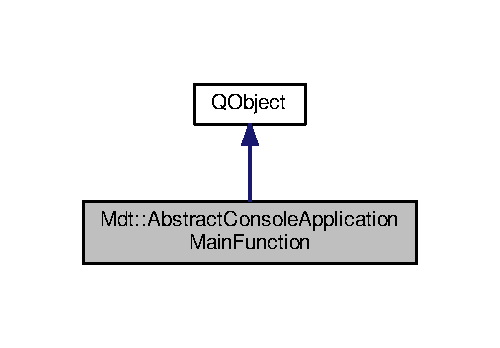
\includegraphics[width=240pt]{class_mdt_1_1_abstract_console_application_main_function__inherit__graph}
\end{center}
\end{figure}


Collaboration diagram for Mdt\+:\+:Abstract\+Console\+Application\+Main\+Function\+:\nopagebreak
\begin{figure}[H]
\begin{center}
\leavevmode
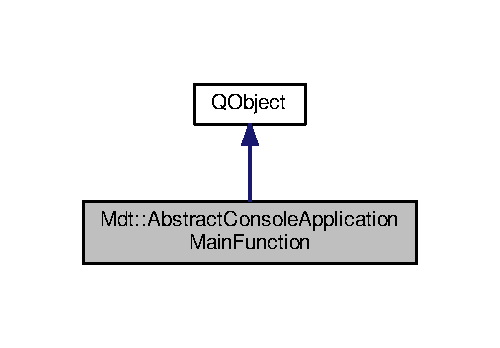
\includegraphics[width=240pt]{class_mdt_1_1_abstract_console_application_main_function__coll__graph}
\end{center}
\end{figure}
\subsection*{Public Slots}
\begin{DoxyCompactItemize}
\item 
virtual void \hyperlink{class_mdt_1_1_abstract_console_application_main_function_a7f00b12d06e341d037cd1a69632b2ac2}{about\+To\+Quit} ()
\begin{DoxyCompactList}\small\item\em Cleanup code. \end{DoxyCompactList}\end{DoxyCompactItemize}
\subsection*{Public Member Functions}
\begin{DoxyCompactItemize}
\item 
\hyperlink{class_mdt_1_1_abstract_console_application_main_function_aec80aaecedd4a2d6696878b96cfc9b40}{Abstract\+Console\+Application\+Main\+Function} (\hyperlink{class_q_object}{Q\+Object} $\ast$parent=nullptr)
\begin{DoxyCompactList}\small\item\em Constructor. \end{DoxyCompactList}\item 
virtual int \hyperlink{class_mdt_1_1_abstract_console_application_main_function_a34213b6ac2188b3620f5c2f5ce4ee287}{run\+Main} ()=0
\begin{DoxyCompactList}\small\item\em main function implementation \end{DoxyCompactList}\end{DoxyCompactItemize}
\subsection*{Static Public Member Functions}
\begin{DoxyCompactItemize}
\item 
static Q\+String\+List \hyperlink{class_mdt_1_1_abstract_console_application_main_function_a4bfe1909139f3c30b03797f7778290fb}{get\+Arguments} ()
\begin{DoxyCompactList}\small\item\em Returns the list of command-\/line arguments. \end{DoxyCompactList}\end{DoxyCompactItemize}


\subsection{Detailed Description}
Abstract base of a main function in Qt console application with a event loop. 

The class declaration My\+Main\+Function.\+h could look like\+: 
\begin{DoxyCode}
\textcolor{keyword}{class }MyMainFunction : \textcolor{keyword}{public} \hyperlink{class_mdt_1_1_abstract_console_application_main_function}{Mdt::AbstractConsoleApplicationMainFunction}
\{
 Q\_OBJECT

 \textcolor{keyword}{public}:

  \textcolor{keyword}{explicit} MyMainFunction(\hyperlink{class_q_object}{QObject}* parent = \textcolor{keyword}{nullptr});
  \textcolor{keywordtype}{int} \hyperlink{class_mdt_1_1_abstract_console_application_main_function_a34213b6ac2188b3620f5c2f5ce4ee287}{runMain}() \textcolor{keyword}{override};
\};
\end{DoxyCode}


Example of the implementation in My\+Main\+Function.\+cpp\+: 
\begin{DoxyCode}
\textcolor{keywordtype}{int} MyMainFunction::runMain()
\{
  qDebug() << \textcolor{stringliteral}{"My main ..."};
\}
\end{DoxyCode}


Finaly, in main.\+cpp\+: 
\begin{DoxyCode}
\hyperlink{class_q_core_application}{QCoreApplication} app(argc, argv);

\textcolor{comment}{// This will call runMain() once the event loop started}
MyMainFunction mainImpl;

\textcolor{keywordflow}{return} app.exec();
\end{DoxyCode}
 

Definition at line 62 of file Abstract\+Console\+Application\+Main\+Function.\+h.



\subsection{Constructor \& Destructor Documentation}
\index{Mdt\+::\+Abstract\+Console\+Application\+Main\+Function@{Mdt\+::\+Abstract\+Console\+Application\+Main\+Function}!Abstract\+Console\+Application\+Main\+Function@{Abstract\+Console\+Application\+Main\+Function}}
\index{Abstract\+Console\+Application\+Main\+Function@{Abstract\+Console\+Application\+Main\+Function}!Mdt\+::\+Abstract\+Console\+Application\+Main\+Function@{Mdt\+::\+Abstract\+Console\+Application\+Main\+Function}}
\subsubsection[{\texorpdfstring{Abstract\+Console\+Application\+Main\+Function(\+Q\+Object $\ast$parent=nullptr)}{AbstractConsoleApplicationMainFunction(QObject *parent=nullptr)}}]{\setlength{\rightskip}{0pt plus 5cm}Mdt\+::\+Abstract\+Console\+Application\+Main\+Function\+::\+Abstract\+Console\+Application\+Main\+Function (
\begin{DoxyParamCaption}
\item[{{\bf Q\+Object} $\ast$}]{parent = {\ttfamily nullptr}}
\end{DoxyParamCaption}
)\hspace{0.3cm}{\ttfamily [explicit]}}\hypertarget{class_mdt_1_1_abstract_console_application_main_function_aec80aaecedd4a2d6696878b96cfc9b40}{}\label{class_mdt_1_1_abstract_console_application_main_function_aec80aaecedd4a2d6696878b96cfc9b40}


Constructor. 



Definition at line 27 of file Abstract\+Console\+Application\+Main\+Function.\+cpp.



\subsection{Member Function Documentation}
\index{Mdt\+::\+Abstract\+Console\+Application\+Main\+Function@{Mdt\+::\+Abstract\+Console\+Application\+Main\+Function}!about\+To\+Quit@{about\+To\+Quit}}
\index{about\+To\+Quit@{about\+To\+Quit}!Mdt\+::\+Abstract\+Console\+Application\+Main\+Function@{Mdt\+::\+Abstract\+Console\+Application\+Main\+Function}}
\subsubsection[{\texorpdfstring{about\+To\+Quit}{aboutToQuit}}]{\setlength{\rightskip}{0pt plus 5cm}void Mdt\+::\+Abstract\+Console\+Application\+Main\+Function\+::about\+To\+Quit (
\begin{DoxyParamCaption}
{}
\end{DoxyParamCaption}
)\hspace{0.3cm}{\ttfamily [virtual]}, {\ttfamily [slot]}}\hypertarget{class_mdt_1_1_abstract_console_application_main_function_a7f00b12d06e341d037cd1a69632b2ac2}{}\label{class_mdt_1_1_abstract_console_application_main_function_a7f00b12d06e341d037cd1a69632b2ac2}


Cleanup code. 

If some cleanup has to be done before the application exists, this function can be implemented. See \hyperlink{class_q_core_application}{Q\+Core\+Application} documentation to know why this is a recommanded way to do cleanup.

This default implementation does nothing. 

Definition at line 41 of file Abstract\+Console\+Application\+Main\+Function.\+cpp.

\index{Mdt\+::\+Abstract\+Console\+Application\+Main\+Function@{Mdt\+::\+Abstract\+Console\+Application\+Main\+Function}!get\+Arguments@{get\+Arguments}}
\index{get\+Arguments@{get\+Arguments}!Mdt\+::\+Abstract\+Console\+Application\+Main\+Function@{Mdt\+::\+Abstract\+Console\+Application\+Main\+Function}}
\subsubsection[{\texorpdfstring{get\+Arguments()}{getArguments()}}]{\setlength{\rightskip}{0pt plus 5cm}Q\+String\+List Mdt\+::\+Abstract\+Console\+Application\+Main\+Function\+::get\+Arguments (
\begin{DoxyParamCaption}
{}
\end{DoxyParamCaption}
)\hspace{0.3cm}{\ttfamily [static]}}\hypertarget{class_mdt_1_1_abstract_console_application_main_function_a4bfe1909139f3c30b03797f7778290fb}{}\label{class_mdt_1_1_abstract_console_application_main_function_a4bfe1909139f3c30b03797f7778290fb}


Returns the list of command-\/line arguments. 

Returns Q\+Core\+Application\+::arguments(). As stated in \hyperlink{class_q_core_application}{Q\+Core\+Application} documentation, this method is slow, so the result should be stored in a variable if accessed many times (this is wy it is prefixed with get here)

\begin{DoxyPrecond}{Precondition}
A instance of a \hyperlink{class_q_core_application}{Q\+Core\+Application} (or one of its derivate) must exist. 
\end{DoxyPrecond}


Definition at line 34 of file Abstract\+Console\+Application\+Main\+Function.\+cpp.

\index{Mdt\+::\+Abstract\+Console\+Application\+Main\+Function@{Mdt\+::\+Abstract\+Console\+Application\+Main\+Function}!run\+Main@{run\+Main}}
\index{run\+Main@{run\+Main}!Mdt\+::\+Abstract\+Console\+Application\+Main\+Function@{Mdt\+::\+Abstract\+Console\+Application\+Main\+Function}}
\subsubsection[{\texorpdfstring{run\+Main()=0}{runMain()=0}}]{\setlength{\rightskip}{0pt plus 5cm}virtual int Mdt\+::\+Abstract\+Console\+Application\+Main\+Function\+::run\+Main (
\begin{DoxyParamCaption}
{}
\end{DoxyParamCaption}
)\hspace{0.3cm}{\ttfamily [pure virtual]}}\hypertarget{class_mdt_1_1_abstract_console_application_main_function_a34213b6ac2188b3620f5c2f5ce4ee287}{}\label{class_mdt_1_1_abstract_console_application_main_function_a34213b6ac2188b3620f5c2f5ce4ee287}


main function implementation 



The documentation for this class was generated from the following files\+:\begin{DoxyCompactItemize}
\item 
libs/\+Application\+\_\+\+Core/src/\+Mdt/Abstract\+Console\+Application\+Main\+Function.\+h\item 
libs/\+Application\+\_\+\+Core/src/\+Mdt/Abstract\+Console\+Application\+Main\+Function.\+cpp\end{DoxyCompactItemize}

\hypertarget{class_mdt_1_1_error_logger_1_1_backend}{}\section{Mdt\+:\+:Error\+Logger\+:\+:Backend Class Reference}
\label{class_mdt_1_1_error_logger_1_1_backend}\index{Mdt\+::\+Error\+Logger\+::\+Backend@{Mdt\+::\+Error\+Logger\+::\+Backend}}


\hyperlink{class_mdt_1_1_error}{Error} \hyperlink{class_mdt_1_1_error_logger_1_1_logger}{Logger} backend.  




{\ttfamily \#include $<$Backend.\+h$>$}



Inheritance diagram for Mdt\+:\+:Error\+Logger\+:\+:Backend\+:
\nopagebreak
\begin{figure}[H]
\begin{center}
\leavevmode
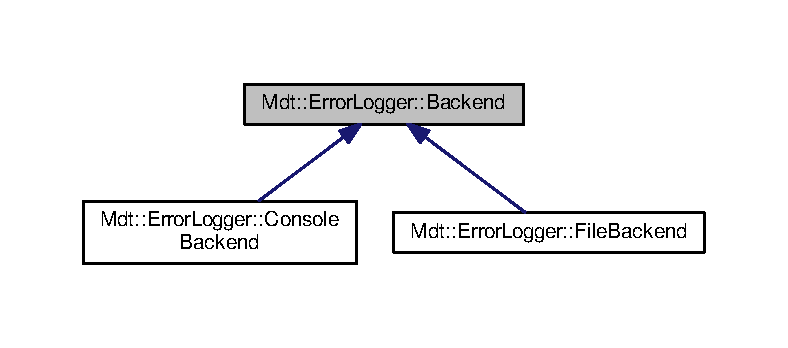
\includegraphics[width=350pt]{class_mdt_1_1_error_logger_1_1_backend__inherit__graph}
\end{center}
\end{figure}
\subsection*{Public Member Functions}
\begin{DoxyCompactItemize}
\item 
\hyperlink{class_mdt_1_1_error_logger_1_1_backend_acf0b4a7f061c638207bfdb172fc8015c}{Backend} ()
\begin{DoxyCompactList}\small\item\em Constructor. \end{DoxyCompactList}\item 
virtual \hyperlink{class_mdt_1_1_error_logger_1_1_backend_aba972e76fc4d6bb7665038cb8d1c88d7}{$\sim$\+Backend} ()
\begin{DoxyCompactList}\small\item\em Destructor. \end{DoxyCompactList}\item 
virtual void \hyperlink{class_mdt_1_1_error_logger_1_1_backend_acf37cfc576269934ca8ce04e3601058d}{log\+Error} (const \hyperlink{class_mdt_1_1_error}{Error} \&error)=0
\begin{DoxyCompactList}\small\item\em Log given error. \end{DoxyCompactList}\item 
{\bfseries Backend} (const \hyperlink{class_mdt_1_1_error_logger_1_1_backend}{Backend} \&)=delete\hypertarget{class_mdt_1_1_error_logger_1_1_backend_a7bb295be149f2205fe63554e1ba06f66}{}\label{class_mdt_1_1_error_logger_1_1_backend_a7bb295be149f2205fe63554e1ba06f66}

\item 
{\bfseries Backend} (\hyperlink{class_mdt_1_1_error_logger_1_1_backend}{Backend} \&\&)=delete\hypertarget{class_mdt_1_1_error_logger_1_1_backend_aba1ff6190a3b08ca93e8edd7917a7d25}{}\label{class_mdt_1_1_error_logger_1_1_backend_aba1ff6190a3b08ca93e8edd7917a7d25}

\item 
\hyperlink{class_mdt_1_1_error_logger_1_1_backend}{Backend} \& {\bfseries operator=} (const \hyperlink{class_mdt_1_1_error_logger_1_1_backend}{Backend} \&)=delete\hypertarget{class_mdt_1_1_error_logger_1_1_backend_a9400fcafaec1e9e07da2d31dcc842b92}{}\label{class_mdt_1_1_error_logger_1_1_backend_a9400fcafaec1e9e07da2d31dcc842b92}

\item 
\hyperlink{class_mdt_1_1_error_logger_1_1_backend}{Backend} \& {\bfseries operator=} (\hyperlink{class_mdt_1_1_error_logger_1_1_backend}{Backend} \&\&)=delete\hypertarget{class_mdt_1_1_error_logger_1_1_backend_ae0beab19d09a61f83eb5feed501a7562}{}\label{class_mdt_1_1_error_logger_1_1_backend_ae0beab19d09a61f83eb5feed501a7562}

\end{DoxyCompactItemize}
\subsection*{Static Protected Member Functions}
\begin{DoxyCompactItemize}
\item 
static Q\+String \hyperlink{class_mdt_1_1_error_logger_1_1_backend_a4a859ea87b93082e69791bcbd14c1f71}{tr} (const char $\ast$text)
\begin{DoxyCompactList}\small\item\em Calls Q\+Object\+::tr() \end{DoxyCompactList}\end{DoxyCompactItemize}


\subsection{Detailed Description}
\hyperlink{class_mdt_1_1_error}{Error} \hyperlink{class_mdt_1_1_error_logger_1_1_logger}{Logger} backend. 

This class is a interface to create a error logger backend that will be used by error \hyperlink{class_mdt_1_1_error_logger_1_1_logger}{Logger} to output errors.

Notice that \hyperlink{class_mdt_1_1_error_logger_1_1_logger}{Logger} executes from a non main thread, also take care that some functons must at least be reentrant. 

Definition at line 40 of file Backend.\+h.



\subsection{Constructor \& Destructor Documentation}
\index{Mdt\+::\+Error\+Logger\+::\+Backend@{Mdt\+::\+Error\+Logger\+::\+Backend}!Backend@{Backend}}
\index{Backend@{Backend}!Mdt\+::\+Error\+Logger\+::\+Backend@{Mdt\+::\+Error\+Logger\+::\+Backend}}
\subsubsection[{\texorpdfstring{Backend()}{Backend()}}]{\setlength{\rightskip}{0pt plus 5cm}Mdt\+::\+Error\+Logger\+::\+Backend\+::\+Backend (
\begin{DoxyParamCaption}
{}
\end{DoxyParamCaption}
)\hspace{0.3cm}{\ttfamily [inline]}}\hypertarget{class_mdt_1_1_error_logger_1_1_backend_acf0b4a7f061c638207bfdb172fc8015c}{}\label{class_mdt_1_1_error_logger_1_1_backend_acf0b4a7f061c638207bfdb172fc8015c}


Constructor. 



Definition at line 46 of file Backend.\+h.



Referenced by $\sim$\+Backend().

\index{Mdt\+::\+Error\+Logger\+::\+Backend@{Mdt\+::\+Error\+Logger\+::\+Backend}!````~Backend@{$\sim$\+Backend}}
\index{````~Backend@{$\sim$\+Backend}!Mdt\+::\+Error\+Logger\+::\+Backend@{Mdt\+::\+Error\+Logger\+::\+Backend}}
\subsubsection[{\texorpdfstring{$\sim$\+Backend()}{~Backend()}}]{\setlength{\rightskip}{0pt plus 5cm}virtual Mdt\+::\+Error\+Logger\+::\+Backend\+::$\sim$\+Backend (
\begin{DoxyParamCaption}
{}
\end{DoxyParamCaption}
)\hspace{0.3cm}{\ttfamily [inline]}, {\ttfamily [virtual]}}\hypertarget{class_mdt_1_1_error_logger_1_1_backend_aba972e76fc4d6bb7665038cb8d1c88d7}{}\label{class_mdt_1_1_error_logger_1_1_backend_aba972e76fc4d6bb7665038cb8d1c88d7}


Destructor. 



Definition at line 50 of file Backend.\+h.



References Backend(), log\+Error(), and tr().



\subsection{Member Function Documentation}
\index{Mdt\+::\+Error\+Logger\+::\+Backend@{Mdt\+::\+Error\+Logger\+::\+Backend}!log\+Error@{log\+Error}}
\index{log\+Error@{log\+Error}!Mdt\+::\+Error\+Logger\+::\+Backend@{Mdt\+::\+Error\+Logger\+::\+Backend}}
\subsubsection[{\texorpdfstring{log\+Error(const Error \&error)=0}{logError(const Error &error)=0}}]{\setlength{\rightskip}{0pt plus 5cm}virtual void Mdt\+::\+Error\+Logger\+::\+Backend\+::log\+Error (
\begin{DoxyParamCaption}
\item[{const {\bf Error} \&}]{error}
\end{DoxyParamCaption}
)\hspace{0.3cm}{\ttfamily [pure virtual]}}\hypertarget{class_mdt_1_1_error_logger_1_1_backend_acf37cfc576269934ca8ce04e3601058d}{}\label{class_mdt_1_1_error_logger_1_1_backend_acf37cfc576269934ca8ce04e3601058d}


Log given error. 

This function must be reentrant, because its called from \hyperlink{class_mdt_1_1_error_logger_1_1_logger}{Logger} thread (witch is not the main thread). 

Implemented in \hyperlink{class_mdt_1_1_error_logger_1_1_file_backend_a31b8314d523a491b5441276122daed87}{Mdt\+::\+Error\+Logger\+::\+File\+Backend}, and \hyperlink{class_mdt_1_1_error_logger_1_1_console_backend_a2d30700dd6a91c244d68bd3670fdbc33}{Mdt\+::\+Error\+Logger\+::\+Console\+Backend}.



Referenced by $\sim$\+Backend().

\index{Mdt\+::\+Error\+Logger\+::\+Backend@{Mdt\+::\+Error\+Logger\+::\+Backend}!tr@{tr}}
\index{tr@{tr}!Mdt\+::\+Error\+Logger\+::\+Backend@{Mdt\+::\+Error\+Logger\+::\+Backend}}
\subsubsection[{\texorpdfstring{tr(const char $\ast$text)}{tr(const char *text)}}]{\setlength{\rightskip}{0pt plus 5cm}Q\+String Mdt\+::\+Error\+Logger\+::\+Backend\+::tr (
\begin{DoxyParamCaption}
\item[{const char $\ast$}]{text}
\end{DoxyParamCaption}
)\hspace{0.3cm}{\ttfamily [static]}, {\ttfamily [protected]}}\hypertarget{class_mdt_1_1_error_logger_1_1_backend_a4a859ea87b93082e69791bcbd14c1f71}{}\label{class_mdt_1_1_error_logger_1_1_backend_a4a859ea87b93082e69791bcbd14c1f71}


Calls Q\+Object\+::tr() 



Definition at line 24 of file Backend.\+cpp.



Referenced by Mdt\+::\+Error\+Logger\+::\+Console\+Backend\+::log\+Error(), Mdt\+::\+Error\+Logger\+::\+File\+Backend\+::log\+Error(), Mdt\+::\+Error\+Logger\+::\+File\+Backend\+::set\+Log\+File\+Path(), and $\sim$\+Backend().



The documentation for this class was generated from the following files\+:\begin{DoxyCompactItemize}
\item 
libs/\+Error\+\_\+\+Core/src/\+Mdt/\+Error\+Logger/Backend.\+h\item 
libs/\+Error\+\_\+\+Core/src/\+Mdt/\+Error\+Logger/Backend.\+cpp\end{DoxyCompactItemize}

\hypertarget{class_mdt_1_1_error_logger_1_1_console_backend}{}\section{Mdt\+:\+:Error\+Logger\+:\+:Console\+Backend Class Reference}
\label{class_mdt_1_1_error_logger_1_1_console_backend}\index{Mdt\+::\+Error\+Logger\+::\+Console\+Backend@{Mdt\+::\+Error\+Logger\+::\+Console\+Backend}}


Console backend for error \hyperlink{class_mdt_1_1_error_logger_1_1_logger}{Logger}.  




{\ttfamily \#include $<$Console\+Backend.\+h$>$}



Inheritance diagram for Mdt\+:\+:Error\+Logger\+:\+:Console\+Backend\+:
\nopagebreak
\begin{figure}[H]
\begin{center}
\leavevmode
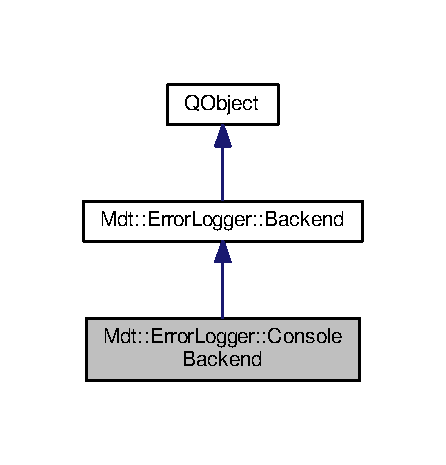
\includegraphics[width=214pt]{class_mdt_1_1_error_logger_1_1_console_backend__inherit__graph}
\end{center}
\end{figure}


Collaboration diagram for Mdt\+:\+:Error\+Logger\+:\+:Console\+Backend\+:
\nopagebreak
\begin{figure}[H]
\begin{center}
\leavevmode
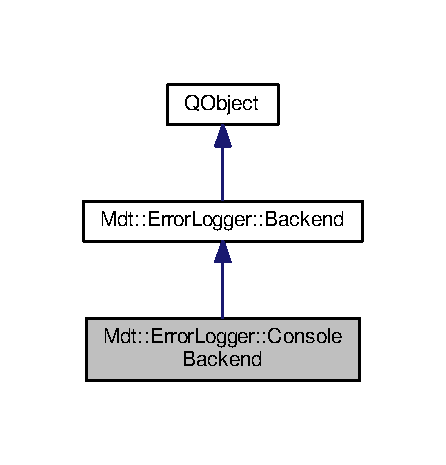
\includegraphics[width=214pt]{class_mdt_1_1_error_logger_1_1_console_backend__coll__graph}
\end{center}
\end{figure}
\subsection*{Public Member Functions}
\begin{DoxyCompactItemize}
\item 
\hyperlink{class_mdt_1_1_error_logger_1_1_console_backend_a79446af5d7658fba5075131f2a0b10dd}{Console\+Backend} (Q\+Object $\ast$parent=nullptr)
\begin{DoxyCompactList}\small\item\em Constructor. \end{DoxyCompactList}\item 
\hyperlink{class_mdt_1_1_error_logger_1_1_console_backend_a7ac5878daa1e4204884d62c592de0e57}{$\sim$\+Console\+Backend} ()
\begin{DoxyCompactList}\small\item\em Destructor. \end{DoxyCompactList}\item 
void \hyperlink{class_mdt_1_1_error_logger_1_1_console_backend_a2d30700dd6a91c244d68bd3670fdbc33}{log\+Error} (const \hyperlink{class_mdt_1_1_error}{Error} \&error)
\begin{DoxyCompactList}\small\item\em Log given error. \end{DoxyCompactList}\end{DoxyCompactItemize}
\subsection*{Additional Inherited Members}


\subsection{Detailed Description}
Console backend for error \hyperlink{class_mdt_1_1_error_logger_1_1_logger}{Logger}. 

Definition at line 31 of file Console\+Backend.\+h.



\subsection{Constructor \& Destructor Documentation}
\index{Mdt\+::\+Error\+Logger\+::\+Console\+Backend@{Mdt\+::\+Error\+Logger\+::\+Console\+Backend}!Console\+Backend@{Console\+Backend}}
\index{Console\+Backend@{Console\+Backend}!Mdt\+::\+Error\+Logger\+::\+Console\+Backend@{Mdt\+::\+Error\+Logger\+::\+Console\+Backend}}
\subsubsection[{\texorpdfstring{Console\+Backend(\+Q\+Object $\ast$parent=nullptr)}{ConsoleBackend(QObject *parent=nullptr)}}]{\setlength{\rightskip}{0pt plus 5cm}Mdt\+::\+Error\+Logger\+::\+Console\+Backend\+::\+Console\+Backend (
\begin{DoxyParamCaption}
\item[{Q\+Object $\ast$}]{parent = {\ttfamily nullptr}}
\end{DoxyParamCaption}
)}\hypertarget{class_mdt_1_1_error_logger_1_1_console_backend_a79446af5d7658fba5075131f2a0b10dd}{}\label{class_mdt_1_1_error_logger_1_1_console_backend_a79446af5d7658fba5075131f2a0b10dd}


Constructor. 



Definition at line 30 of file Console\+Backend.\+cpp.

\index{Mdt\+::\+Error\+Logger\+::\+Console\+Backend@{Mdt\+::\+Error\+Logger\+::\+Console\+Backend}!````~Console\+Backend@{$\sim$\+Console\+Backend}}
\index{````~Console\+Backend@{$\sim$\+Console\+Backend}!Mdt\+::\+Error\+Logger\+::\+Console\+Backend@{Mdt\+::\+Error\+Logger\+::\+Console\+Backend}}
\subsubsection[{\texorpdfstring{$\sim$\+Console\+Backend()}{~ConsoleBackend()}}]{\setlength{\rightskip}{0pt plus 5cm}Mdt\+::\+Error\+Logger\+::\+Console\+Backend\+::$\sim$\+Console\+Backend (
\begin{DoxyParamCaption}
{}
\end{DoxyParamCaption}
)}\hypertarget{class_mdt_1_1_error_logger_1_1_console_backend_a7ac5878daa1e4204884d62c592de0e57}{}\label{class_mdt_1_1_error_logger_1_1_console_backend_a7ac5878daa1e4204884d62c592de0e57}


Destructor. 



Definition at line 35 of file Console\+Backend.\+cpp.



\subsection{Member Function Documentation}
\index{Mdt\+::\+Error\+Logger\+::\+Console\+Backend@{Mdt\+::\+Error\+Logger\+::\+Console\+Backend}!log\+Error@{log\+Error}}
\index{log\+Error@{log\+Error}!Mdt\+::\+Error\+Logger\+::\+Console\+Backend@{Mdt\+::\+Error\+Logger\+::\+Console\+Backend}}
\subsubsection[{\texorpdfstring{log\+Error(const Error \&error)}{logError(const Error &error)}}]{\setlength{\rightskip}{0pt plus 5cm}void Mdt\+::\+Error\+Logger\+::\+Console\+Backend\+::log\+Error (
\begin{DoxyParamCaption}
\item[{const {\bf Error} \&}]{error}
\end{DoxyParamCaption}
)\hspace{0.3cm}{\ttfamily [virtual]}}\hypertarget{class_mdt_1_1_error_logger_1_1_console_backend_a2d30700dd6a91c244d68bd3670fdbc33}{}\label{class_mdt_1_1_error_logger_1_1_console_backend_a2d30700dd6a91c244d68bd3670fdbc33}


Log given error. 



Implements \hyperlink{class_mdt_1_1_error_logger_1_1_backend_acf37cfc576269934ca8ce04e3601058d}{Mdt\+::\+Error\+Logger\+::\+Backend}.



Definition at line 39 of file Console\+Backend.\+cpp.



The documentation for this class was generated from the following files\+:\begin{DoxyCompactItemize}
\item 
libs/\+Error\+\_\+\+Core/src/\+Mdt/\+Error\+Logger/Console\+Backend.\+h\item 
libs/\+Error\+\_\+\+Core/src/\+Mdt/\+Error\+Logger/Console\+Backend.\+cpp\end{DoxyCompactItemize}

\hypertarget{class_mdt_1_1_core_application}{}\section{Mdt\+:\+:Core\+Application Class Reference}
\label{class_mdt_1_1_core_application}\index{Mdt\+::\+Core\+Application@{Mdt\+::\+Core\+Application}}


\hyperlink{class_mdt_1_1_core_application}{Core\+Application} adds some helper to \hyperlink{class_q_core_application}{Q\+Core\+Application} for application initialization.  




{\ttfamily \#include $<$Core\+Application.\+h$>$}



Inheritance diagram for Mdt\+:\+:Core\+Application\+:
\nopagebreak
\begin{figure}[H]
\begin{center}
\leavevmode
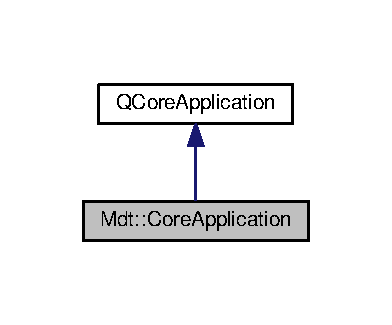
\includegraphics[width=188pt]{class_mdt_1_1_core_application__inherit__graph}
\end{center}
\end{figure}


Collaboration diagram for Mdt\+:\+:Core\+Application\+:
\nopagebreak
\begin{figure}[H]
\begin{center}
\leavevmode
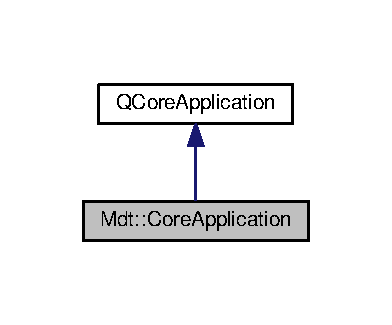
\includegraphics[width=188pt]{class_mdt_1_1_core_application__coll__graph}
\end{center}
\end{figure}
\subsection*{Public Member Functions}
\begin{DoxyCompactItemize}
\item 
\hyperlink{class_mdt_1_1_core_application_a1f9e0cee5d94ec783ea49ec57030bce9}{Core\+Application} (int \&argc, char $\ast$$\ast$argv)
\begin{DoxyCompactList}\small\item\em Construct a core application. \end{DoxyCompactList}\item 
\hyperlink{class_mdt_1_1_core_application_ac91f0fe77618f10cbdf1f5594c2a82ea}{$\sim$\+Core\+Application} ()
\begin{DoxyCompactList}\small\item\em Destroy the core application object. \end{DoxyCompactList}\item 
{\bfseries Core\+Application} (const \hyperlink{class_mdt_1_1_core_application}{Core\+Application} \&)=delete\hypertarget{class_mdt_1_1_core_application_a62325e06671365f59e2e665d154c7980}{}\label{class_mdt_1_1_core_application_a62325e06671365f59e2e665d154c7980}

\item 
\hyperlink{class_mdt_1_1_core_application}{Core\+Application} \& {\bfseries operator=} (const \hyperlink{class_mdt_1_1_core_application}{Core\+Application} \&)=delete\hypertarget{class_mdt_1_1_core_application_a7d289e822b3b564ec1be514f1abe8634}{}\label{class_mdt_1_1_core_application_a7d289e822b3b564ec1be514f1abe8634}

\item 
{\bfseries Core\+Application} (\hyperlink{class_mdt_1_1_core_application}{Core\+Application} \&\&)=delete\hypertarget{class_mdt_1_1_core_application_add05d6ef32f7eaf59573a1d5a1a3e488}{}\label{class_mdt_1_1_core_application_add05d6ef32f7eaf59573a1d5a1a3e488}

\item 
\hyperlink{class_mdt_1_1_core_application}{Core\+Application} \& {\bfseries operator=} (\hyperlink{class_mdt_1_1_core_application}{Core\+Application} \&\&)=delete\hypertarget{class_mdt_1_1_core_application_aceac66ce619e99eba6fbf1039da9a009}{}\label{class_mdt_1_1_core_application_aceac66ce619e99eba6fbf1039da9a009}

\item 
void \hyperlink{class_mdt_1_1_core_application_aa76faa75f09c7ba30406bfd6b2284bd7}{enable\+File\+Logging} ()
\begin{DoxyCompactList}\small\item\em Enable file logging. \end{DoxyCompactList}\item 
Q\+String \hyperlink{class_mdt_1_1_core_application_a48a2915a7876c259347290f1f501df46}{log\+File\+Path} ()
\begin{DoxyCompactList}\small\item\em Get the path to the log file. \end{DoxyCompactList}\item 
void \hyperlink{class_mdt_1_1_core_application_a500820026134788b2c77c880663339d9}{debug\+Environment} ()
\begin{DoxyCompactList}\small\item\em Debug environment. \end{DoxyCompactList}\end{DoxyCompactItemize}
\subsection*{Static Public Member Functions}
\begin{DoxyCompactItemize}
\item 
static Q\+String \hyperlink{class_mdt_1_1_core_application_aa5bf79da0eda7f8dedd2b78bf8025449}{cache\+Directory\+Path} ()
\begin{DoxyCompactList}\small\item\em Get path to the cache directory. \end{DoxyCompactList}\item 
static Q\+String \hyperlink{class_mdt_1_1_core_application_a0509073283a3a23e4ee3cf248739e15c}{qt\+Version} ()
\begin{DoxyCompactList}\small\item\em Get Qt library version. \end{DoxyCompactList}\item 
static Q\+String \hyperlink{class_mdt_1_1_core_application_a43d5e4e3b163250cba37c0071fb9f7ea}{mdt\+Version} ()
\begin{DoxyCompactList}\small\item\em Get \hyperlink{namespace_mdt}{Mdt} library version. \end{DoxyCompactList}\end{DoxyCompactItemize}


\subsection{Detailed Description}
\hyperlink{class_mdt_1_1_core_application}{Core\+Application} adds some helper to \hyperlink{class_q_core_application}{Q\+Core\+Application} for application initialization. 

\begin{DoxySeeAlso}{See also}
\hyperlink{class_q_core_application}{Q\+Core\+Application} 
\end{DoxySeeAlso}


Definition at line 36 of file Core\+Application.\+h.



\subsection{Constructor \& Destructor Documentation}
\index{Mdt\+::\+Core\+Application@{Mdt\+::\+Core\+Application}!Core\+Application@{Core\+Application}}
\index{Core\+Application@{Core\+Application}!Mdt\+::\+Core\+Application@{Mdt\+::\+Core\+Application}}
\subsubsection[{\texorpdfstring{Core\+Application(int \&argc, char $\ast$$\ast$argv)}{CoreApplication(int &argc, char **argv)}}]{\setlength{\rightskip}{0pt plus 5cm}Mdt\+::\+Core\+Application\+::\+Core\+Application (
\begin{DoxyParamCaption}
\item[{int \&}]{argc, }
\item[{char $\ast$$\ast$}]{argv}
\end{DoxyParamCaption}
)}\hypertarget{class_mdt_1_1_core_application_a1f9e0cee5d94ec783ea49ec57030bce9}{}\label{class_mdt_1_1_core_application_a1f9e0cee5d94ec783ea49ec57030bce9}


Construct a core application. 



Definition at line 26 of file Core\+Application.\+cpp.

\index{Mdt\+::\+Core\+Application@{Mdt\+::\+Core\+Application}!````~Core\+Application@{$\sim$\+Core\+Application}}
\index{````~Core\+Application@{$\sim$\+Core\+Application}!Mdt\+::\+Core\+Application@{Mdt\+::\+Core\+Application}}
\subsubsection[{\texorpdfstring{$\sim$\+Core\+Application()}{~CoreApplication()}}]{\setlength{\rightskip}{0pt plus 5cm}Mdt\+::\+Core\+Application\+::$\sim$\+Core\+Application (
\begin{DoxyParamCaption}
{}
\end{DoxyParamCaption}
)}\hypertarget{class_mdt_1_1_core_application_ac91f0fe77618f10cbdf1f5594c2a82ea}{}\label{class_mdt_1_1_core_application_ac91f0fe77618f10cbdf1f5594c2a82ea}


Destroy the core application object. 



Definition at line 32 of file Core\+Application.\+cpp.



\subsection{Member Function Documentation}
\index{Mdt\+::\+Core\+Application@{Mdt\+::\+Core\+Application}!cache\+Directory\+Path@{cache\+Directory\+Path}}
\index{cache\+Directory\+Path@{cache\+Directory\+Path}!Mdt\+::\+Core\+Application@{Mdt\+::\+Core\+Application}}
\subsubsection[{\texorpdfstring{cache\+Directory\+Path()}{cacheDirectoryPath()}}]{\setlength{\rightskip}{0pt plus 5cm}Q\+String Mdt\+::\+Core\+Application\+::cache\+Directory\+Path (
\begin{DoxyParamCaption}
{}
\end{DoxyParamCaption}
)\hspace{0.3cm}{\ttfamily [static]}}\hypertarget{class_mdt_1_1_core_application_aa5bf79da0eda7f8dedd2b78bf8025449}{}\label{class_mdt_1_1_core_application_aa5bf79da0eda7f8dedd2b78bf8025449}


Get path to the cache directory. 

Returns \hyperlink{class_mdt_1_1_standard_paths_a2ca803e5a6b9fb2a4808968becfb86de}{Standard\+Paths\+::cache\+Directory\+Path()} 

Definition at line 46 of file Core\+Application.\+cpp.



References Mdt\+::\+Core\+Application\+Impl\+::cache\+Directory\+Path().

\index{Mdt\+::\+Core\+Application@{Mdt\+::\+Core\+Application}!debug\+Environment@{debug\+Environment}}
\index{debug\+Environment@{debug\+Environment}!Mdt\+::\+Core\+Application@{Mdt\+::\+Core\+Application}}
\subsubsection[{\texorpdfstring{debug\+Environment()}{debugEnvironment()}}]{\setlength{\rightskip}{0pt plus 5cm}void Mdt\+::\+Core\+Application\+::debug\+Environment (
\begin{DoxyParamCaption}
{}
\end{DoxyParamCaption}
)}\hypertarget{class_mdt_1_1_core_application_a500820026134788b2c77c880663339d9}{}\label{class_mdt_1_1_core_application_a500820026134788b2c77c880663339d9}


Debug environment. 

Will print various informations, like libraries versions, paths to some directories, etc.. to the console. 

Definition at line 61 of file Core\+Application.\+cpp.

\index{Mdt\+::\+Core\+Application@{Mdt\+::\+Core\+Application}!enable\+File\+Logging@{enable\+File\+Logging}}
\index{enable\+File\+Logging@{enable\+File\+Logging}!Mdt\+::\+Core\+Application@{Mdt\+::\+Core\+Application}}
\subsubsection[{\texorpdfstring{enable\+File\+Logging()}{enableFileLogging()}}]{\setlength{\rightskip}{0pt plus 5cm}void Mdt\+::\+Core\+Application\+::enable\+File\+Logging (
\begin{DoxyParamCaption}
{}
\end{DoxyParamCaption}
)}\hypertarget{class_mdt_1_1_core_application_aa76faa75f09c7ba30406bfd6b2284bd7}{}\label{class_mdt_1_1_core_application_aa76faa75f09c7ba30406bfd6b2284bd7}


Enable file logging. 

After file logging was enabled, errors that are committed using \hyperlink{class_mdt_1_1_error_a1b4a57bd4177d2985abd62b6b49a43f8}{Mdt\+::\+Error\+::commit()} are added to the log file {\itshape \hyperlink{class_mdt_1_1_core_application_a48a2915a7876c259347290f1f501df46}{log\+File\+Path()}} . 

Definition at line 36 of file Core\+Application.\+cpp.



References Mdt\+::\+Core\+Application\+Impl\+::\+Application\+Name\+And\+Pid.

\index{Mdt\+::\+Core\+Application@{Mdt\+::\+Core\+Application}!log\+File\+Path@{log\+File\+Path}}
\index{log\+File\+Path@{log\+File\+Path}!Mdt\+::\+Core\+Application@{Mdt\+::\+Core\+Application}}
\subsubsection[{\texorpdfstring{log\+File\+Path()}{logFilePath()}}]{\setlength{\rightskip}{0pt plus 5cm}Q\+String Mdt\+::\+Core\+Application\+::log\+File\+Path (
\begin{DoxyParamCaption}
{}
\end{DoxyParamCaption}
)}\hypertarget{class_mdt_1_1_core_application_a48a2915a7876c259347290f1f501df46}{}\label{class_mdt_1_1_core_application_a48a2915a7876c259347290f1f501df46}


Get the path to the log file. 



Definition at line 41 of file Core\+Application.\+cpp.

\index{Mdt\+::\+Core\+Application@{Mdt\+::\+Core\+Application}!mdt\+Version@{mdt\+Version}}
\index{mdt\+Version@{mdt\+Version}!Mdt\+::\+Core\+Application@{Mdt\+::\+Core\+Application}}
\subsubsection[{\texorpdfstring{mdt\+Version()}{mdtVersion()}}]{\setlength{\rightskip}{0pt plus 5cm}Q\+String Mdt\+::\+Core\+Application\+::mdt\+Version (
\begin{DoxyParamCaption}
{}
\end{DoxyParamCaption}
)\hspace{0.3cm}{\ttfamily [static]}}\hypertarget{class_mdt_1_1_core_application_a43d5e4e3b163250cba37c0071fb9f7ea}{}\label{class_mdt_1_1_core_application_a43d5e4e3b163250cba37c0071fb9f7ea}


Get \hyperlink{namespace_mdt}{Mdt} library version. 



Definition at line 56 of file Core\+Application.\+cpp.



References Mdt\+::\+Core\+Application\+Impl\+::mdt\+Version().

\index{Mdt\+::\+Core\+Application@{Mdt\+::\+Core\+Application}!qt\+Version@{qt\+Version}}
\index{qt\+Version@{qt\+Version}!Mdt\+::\+Core\+Application@{Mdt\+::\+Core\+Application}}
\subsubsection[{\texorpdfstring{qt\+Version()}{qtVersion()}}]{\setlength{\rightskip}{0pt plus 5cm}Q\+String Mdt\+::\+Core\+Application\+::qt\+Version (
\begin{DoxyParamCaption}
{}
\end{DoxyParamCaption}
)\hspace{0.3cm}{\ttfamily [static]}}\hypertarget{class_mdt_1_1_core_application_a0509073283a3a23e4ee3cf248739e15c}{}\label{class_mdt_1_1_core_application_a0509073283a3a23e4ee3cf248739e15c}


Get Qt library version. 



Definition at line 51 of file Core\+Application.\+cpp.



References Mdt\+::\+Core\+Application\+Impl\+::qt\+Version().



The documentation for this class was generated from the following files\+:\begin{DoxyCompactItemize}
\item 
libs/\+Application\+\_\+\+Core/src/\+Mdt/Core\+Application.\+h\item 
libs/\+Application\+\_\+\+Core/src/\+Mdt/Core\+Application.\+cpp\end{DoxyCompactItemize}

\hypertarget{class_mdt_1_1_core_application_impl}{}\section{Mdt\+:\+:Core\+Application\+Impl Class Reference}
\label{class_mdt_1_1_core_application_impl}\index{Mdt\+::\+Core\+Application\+Impl@{Mdt\+::\+Core\+Application\+Impl}}


Implementation for \hyperlink{class_mdt_1_1_core_application}{Core\+Application} and derived classes.  




{\ttfamily \#include $<$Core\+Application\+Impl.\+h$>$}



Inheritance diagram for Mdt\+:\+:Core\+Application\+Impl\+:\nopagebreak
\begin{figure}[H]
\begin{center}
\leavevmode
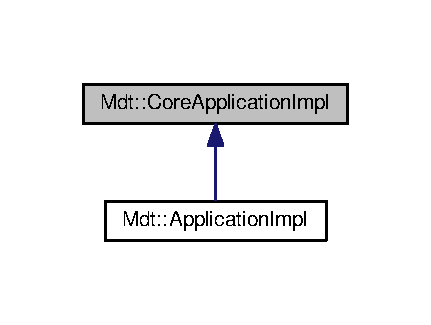
\includegraphics[width=207pt]{class_mdt_1_1_core_application_impl__inherit__graph}
\end{center}
\end{figure}
\subsection*{Public Types}
\subsection*{Public Member Functions}
\begin{DoxyCompactItemize}
\item 
\hyperlink{class_mdt_1_1_core_application_impl_ab97b101b57a2fa8410e39b940e022c4c}{Core\+Application\+Impl} ()\hypertarget{class_mdt_1_1_core_application_impl_ab97b101b57a2fa8410e39b940e022c4c}{}\label{class_mdt_1_1_core_application_impl_ab97b101b57a2fa8410e39b940e022c4c}

\begin{DoxyCompactList}\small\item\em Constructor. \end{DoxyCompactList}\item 
\hyperlink{class_mdt_1_1_core_application_impl_aa17f799e5d756ca8c5a89196fcbd8e90}{$\sim$\+Core\+Application\+Impl} ()\hypertarget{class_mdt_1_1_core_application_impl_aa17f799e5d756ca8c5a89196fcbd8e90}{}\label{class_mdt_1_1_core_application_impl_aa17f799e5d756ca8c5a89196fcbd8e90}

\begin{DoxyCompactList}\small\item\em Destructor. \end{DoxyCompactList}\item 
void \hyperlink{class_mdt_1_1_core_application_impl_a3bd40afeeb08ddcba8cbfc78c177305b}{enable\+File\+Logging} (\hyperlink{class_mdt_1_1_core_application_impl_aa5fed8435e22870a870005ee28ff6221}{Log\+File\+Name\+Format} format)\hypertarget{class_mdt_1_1_core_application_impl_a3bd40afeeb08ddcba8cbfc78c177305b}{}\label{class_mdt_1_1_core_application_impl_a3bd40afeeb08ddcba8cbfc78c177305b}

\begin{DoxyCompactList}\small\item\em Enable file logging. \end{DoxyCompactList}\item 
bool \hyperlink{class_mdt_1_1_core_application_impl_a42a42b5d134b70a6e1c0452f29c73912}{is\+File\+Logging\+Enabled} () const \hypertarget{class_mdt_1_1_core_application_impl_a42a42b5d134b70a6e1c0452f29c73912}{}\label{class_mdt_1_1_core_application_impl_a42a42b5d134b70a6e1c0452f29c73912}

\begin{DoxyCompactList}\small\item\em Check if file logging is enabled. \end{DoxyCompactList}\item 
Q\+String \hyperlink{class_mdt_1_1_core_application_impl_abc2b6b3ab83fdf2fd9dca1447bc82418}{log\+File\+Path} ()\hypertarget{class_mdt_1_1_core_application_impl_abc2b6b3ab83fdf2fd9dca1447bc82418}{}\label{class_mdt_1_1_core_application_impl_abc2b6b3ab83fdf2fd9dca1447bc82418}

\begin{DoxyCompactList}\small\item\em Get the path to the log file. \end{DoxyCompactList}\item 
void \hyperlink{class_mdt_1_1_core_application_impl_a29a336750c7ea04a570fbd769497c98f}{debug\+Environment} (const Q\+String\+List \&entries)\hypertarget{class_mdt_1_1_core_application_impl_a29a336750c7ea04a570fbd769497c98f}{}\label{class_mdt_1_1_core_application_impl_a29a336750c7ea04a570fbd769497c98f}

\begin{DoxyCompactList}\small\item\em Debug environment. \end{DoxyCompactList}\item 
Q\+String\+List \hyperlink{class_mdt_1_1_core_application_impl_abbafc463e7c820e42f967813e9e7ae7a}{common\+Environment\+Entries} ()\hypertarget{class_mdt_1_1_core_application_impl_abbafc463e7c820e42f967813e9e7ae7a}{}\label{class_mdt_1_1_core_application_impl_abbafc463e7c820e42f967813e9e7ae7a}

\begin{DoxyCompactList}\small\item\em Get common environment entries. \end{DoxyCompactList}\end{DoxyCompactItemize}
\subsection*{Static Public Member Functions}
\begin{DoxyCompactItemize}
\item 
static Q\+String \hyperlink{class_mdt_1_1_core_application_impl_a5335fddfbe75c3944199d30d201ece04}{log\+Directory\+Path} ()
\begin{DoxyCompactList}\small\item\em Get the path to log file directory. \end{DoxyCompactList}\item 
static Q\+String \hyperlink{class_mdt_1_1_core_application_impl_a4d78244d773ca265a7108275f2295ca2}{cache\+Directory\+Path} ()
\begin{DoxyCompactList}\small\item\em Get path to the cache directory. \end{DoxyCompactList}\item 
static Q\+String \hyperlink{class_mdt_1_1_core_application_impl_a7c1f7ed8684b4d3ec8aa68a0da5d2d04}{qt\+Version} ()\hypertarget{class_mdt_1_1_core_application_impl_a7c1f7ed8684b4d3ec8aa68a0da5d2d04}{}\label{class_mdt_1_1_core_application_impl_a7c1f7ed8684b4d3ec8aa68a0da5d2d04}

\begin{DoxyCompactList}\small\item\em Get Qt library version. \end{DoxyCompactList}\item 
static Q\+String \hyperlink{class_mdt_1_1_core_application_impl_af8728d7751e6041d5680d99f033ae52d}{mdt\+Version} ()\hypertarget{class_mdt_1_1_core_application_impl_af8728d7751e6041d5680d99f033ae52d}{}\label{class_mdt_1_1_core_application_impl_af8728d7751e6041d5680d99f033ae52d}

\begin{DoxyCompactList}\small\item\em Get \hyperlink{namespace_mdt}{Mdt} library version. \end{DoxyCompactList}\end{DoxyCompactItemize}


\subsection{Detailed Description}
Implementation for \hyperlink{class_mdt_1_1_core_application}{Core\+Application} and derived classes. 

Definition at line 34 of file Core\+Application\+Impl.\+h.



\subsection{Member Enumeration Documentation}
\index{Mdt\+::\+Core\+Application\+Impl@{Mdt\+::\+Core\+Application\+Impl}!Log\+File\+Name\+Format@{Log\+File\+Name\+Format}}
\index{Log\+File\+Name\+Format@{Log\+File\+Name\+Format}!Mdt\+::\+Core\+Application\+Impl@{Mdt\+::\+Core\+Application\+Impl}}
\subsubsection[{\texorpdfstring{Log\+File\+Name\+Format}{LogFileNameFormat}}]{\setlength{\rightskip}{0pt plus 5cm}enum {\bf Mdt\+::\+Core\+Application\+Impl\+::\+Log\+File\+Name\+Format}}\hypertarget{class_mdt_1_1_core_application_impl_aa5fed8435e22870a870005ee28ff6221}{}\label{class_mdt_1_1_core_application_impl_aa5fed8435e22870a870005ee28ff6221}


Log file name format. 

\begin{Desc}
\item[Enumerator]\par
\begin{description}
\index{Application\+Name@{Application\+Name}!Mdt\+::\+Core\+Application\+Impl@{Mdt\+::\+Core\+Application\+Impl}}\index{Mdt\+::\+Core\+Application\+Impl@{Mdt\+::\+Core\+Application\+Impl}!Application\+Name@{Application\+Name}}\item[{\em 
Application\+Name\hypertarget{class_mdt_1_1_core_application_impl_aa5fed8435e22870a870005ee28ff6221ab47da4311e174cd5978c765033f0060e}{}\label{class_mdt_1_1_core_application_impl_aa5fed8435e22870a870005ee28ff6221ab47da4311e174cd5978c765033f0060e}
}]Log file name will be application\+Name.\+log \index{Application\+Name\+And\+Pid@{Application\+Name\+And\+Pid}!Mdt\+::\+Core\+Application\+Impl@{Mdt\+::\+Core\+Application\+Impl}}\index{Mdt\+::\+Core\+Application\+Impl@{Mdt\+::\+Core\+Application\+Impl}!Application\+Name\+And\+Pid@{Application\+Name\+And\+Pid}}\item[{\em 
Application\+Name\+And\+Pid\hypertarget{class_mdt_1_1_core_application_impl_aa5fed8435e22870a870005ee28ff6221ae817e774fbf9d95b9b720ce7da8e6604}{}\label{class_mdt_1_1_core_application_impl_aa5fed8435e22870a870005ee28ff6221ae817e774fbf9d95b9b720ce7da8e6604}
}]Log file name will be application\+Name\+\_\+pid.\+log \end{description}
\end{Desc}


Definition at line 42 of file Core\+Application\+Impl.\+h.



\subsection{Member Function Documentation}
\index{Mdt\+::\+Core\+Application\+Impl@{Mdt\+::\+Core\+Application\+Impl}!cache\+Directory\+Path@{cache\+Directory\+Path}}
\index{cache\+Directory\+Path@{cache\+Directory\+Path}!Mdt\+::\+Core\+Application\+Impl@{Mdt\+::\+Core\+Application\+Impl}}
\subsubsection[{\texorpdfstring{cache\+Directory\+Path()}{cacheDirectoryPath()}}]{\setlength{\rightskip}{0pt plus 5cm}static Q\+String Mdt\+::\+Core\+Application\+Impl\+::cache\+Directory\+Path (
\begin{DoxyParamCaption}
{}
\end{DoxyParamCaption}
)\hspace{0.3cm}{\ttfamily [inline]}, {\ttfamily [static]}}\hypertarget{class_mdt_1_1_core_application_impl_a4d78244d773ca265a7108275f2295ca2}{}\label{class_mdt_1_1_core_application_impl_a4d78244d773ca265a7108275f2295ca2}


Get path to the cache directory. 

Returns \hyperlink{class_mdt_1_1_standard_paths_a2ca803e5a6b9fb2a4808968becfb86de}{Standard\+Paths\+::cache\+Directory\+Path()} 

Definition at line 94 of file Core\+Application\+Impl.\+h.

\index{Mdt\+::\+Core\+Application\+Impl@{Mdt\+::\+Core\+Application\+Impl}!log\+Directory\+Path@{log\+Directory\+Path}}
\index{log\+Directory\+Path@{log\+Directory\+Path}!Mdt\+::\+Core\+Application\+Impl@{Mdt\+::\+Core\+Application\+Impl}}
\subsubsection[{\texorpdfstring{log\+Directory\+Path()}{logDirectoryPath()}}]{\setlength{\rightskip}{0pt plus 5cm}static Q\+String Mdt\+::\+Core\+Application\+Impl\+::log\+Directory\+Path (
\begin{DoxyParamCaption}
{}
\end{DoxyParamCaption}
)\hspace{0.3cm}{\ttfamily [inline]}, {\ttfamily [static]}}\hypertarget{class_mdt_1_1_core_application_impl_a5335fddfbe75c3944199d30d201ece04}{}\label{class_mdt_1_1_core_application_impl_a5335fddfbe75c3944199d30d201ece04}


Get the path to log file directory. 

Returns \hyperlink{class_mdt_1_1_standard_paths_aa45caeb4d2b4a5c539d301d800a7deac}{Standard\+Paths\+::log\+Directory\+Path()} 

Definition at line 78 of file Core\+Application\+Impl.\+h.



The documentation for this class was generated from the following files\+:\begin{DoxyCompactItemize}
\item 
libs/\+Application\+\_\+\+Core/src/\+Mdt/Core\+Application\+Impl.\+h\item 
libs/\+Application\+\_\+\+Core/src/\+Mdt/Core\+Application\+Impl.\+cpp\end{DoxyCompactItemize}

\hypertarget{class_mdt_1_1_error}{}\section{Mdt\+:\+:Error Class Reference}
\label{class_mdt_1_1_error}\index{Mdt\+::\+Error@{Mdt\+::\+Error}}


Value class that contains a error.  




{\ttfamily \#include $<$Error.\+h$>$}

\subsection*{Public Types}
\begin{DoxyCompactItemize}
\item 
enum \hyperlink{class_mdt_1_1_error_ab533dc690f68a8635232db594194a068}{Level} \+: short \{ \hyperlink{class_mdt_1_1_error_ab533dc690f68a8635232db594194a068a1f0076cc77af5bed268bcef0c88969de}{No\+Error}, 
\hyperlink{class_mdt_1_1_error_ab533dc690f68a8635232db594194a068a6cf5d2017767cf4086ebb2d245d42f11}{Info}, 
\hyperlink{class_mdt_1_1_error_ab533dc690f68a8635232db594194a068a6b9dbb52e31678b806f4ecf1ae23d2ab}{Warning}, 
\hyperlink{class_mdt_1_1_error_ab533dc690f68a8635232db594194a068a6d4d123a2a43721c206c455a721567b6}{Critical}
 \}\begin{DoxyCompactList}\small\item\em \hyperlink{class_mdt_1_1_error}{Error} level. \end{DoxyCompactList}
\end{DoxyCompactItemize}
\subsection*{Public Member Functions}
\begin{DoxyCompactItemize}
\item 
\hyperlink{class_mdt_1_1_error_af7cd5683888bc46f9a484670f02520d5}{Error} ()
\begin{DoxyCompactList}\small\item\em Construct a null error. \end{DoxyCompactList}\item 
{\footnotesize template$<$typename T $>$ }\\\hyperlink{class_mdt_1_1_error_ad12894ddf0783443f8351371b701ca89}{Error} (const T \&\hyperlink{class_mdt_1_1_error_a0d042250a76d0351b8c19367572f5e11}{error}, const Q\+String \&\hyperlink{class_mdt_1_1_error_a99327678615e8f2bddd22cd59482bfc2}{text}, \hyperlink{class_mdt_1_1_error_ab533dc690f68a8635232db594194a068}{Level} \hyperlink{class_mdt_1_1_error_a9c73117a49791ab87163b815d6a3e0c9}{level}, const Q\+String \&\hyperlink{class_mdt_1_1_error_a5f7cdab03c2c0955693ace234039cd53}{file\+Name}, int \hyperlink{class_mdt_1_1_error_a5b887edc31341eb23557905e7a2d69ae}{file\+Line}, const Q\+String \&class\+Name, const Q\+String \&\hyperlink{class_mdt_1_1_error_a5706a74669219d9672ee20414f805cab}{function\+Name})
\begin{DoxyCompactList}\small\item\em Construct a error with error and source set. \end{DoxyCompactList}\item 
{\footnotesize template$<$typename T $>$ }\\\hyperlink{class_mdt_1_1_error_a8643711dcae19d29e332b10b5420dd21}{Error} (const T \&\hyperlink{class_mdt_1_1_error_a0d042250a76d0351b8c19367572f5e11}{error}, const Q\+String \&\hyperlink{class_mdt_1_1_error_a99327678615e8f2bddd22cd59482bfc2}{text}, \hyperlink{class_mdt_1_1_error_ab533dc690f68a8635232db594194a068}{Level} \hyperlink{class_mdt_1_1_error_a9c73117a49791ab87163b815d6a3e0c9}{level}, const Q\+String \&\hyperlink{class_mdt_1_1_error_a5f7cdab03c2c0955693ace234039cd53}{file\+Name}, int \hyperlink{class_mdt_1_1_error_a5b887edc31341eb23557905e7a2d69ae}{file\+Line}, const \hyperlink{class_q_object}{Q\+Object} $\ast$const obj, const Q\+String \&\hyperlink{class_mdt_1_1_error_a5706a74669219d9672ee20414f805cab}{function\+Name})
\begin{DoxyCompactList}\small\item\em Construct a error with error and source set. \end{DoxyCompactList}\item 
\hyperlink{class_mdt_1_1_error_a7d7baf19eba7c6f5fb446a919fe8ee41}{Error} (const \hyperlink{class_mdt_1_1_error}{Error} \&)=default
\begin{DoxyCompactList}\small\item\em Construct a copy of other error. \end{DoxyCompactList}\item 
bool \hyperlink{class_mdt_1_1_error_a2b6a7708216d0de056c7d9e7dc571e70}{is\+Null} () const 
\begin{DoxyCompactList}\small\item\em Check if error is null. \end{DoxyCompactList}\item 
void \hyperlink{class_mdt_1_1_error_a77014ce33160e1f01b3fbb3e55f19783}{clear} ()
\begin{DoxyCompactList}\small\item\em Clear error. \end{DoxyCompactList}\item 
void \hyperlink{class_mdt_1_1_error_a895930ac30664f54a7f22ae593db53a0}{set\+Error} (const Q\+String \&\hyperlink{class_mdt_1_1_error_a99327678615e8f2bddd22cd59482bfc2}{text}, \hyperlink{class_mdt_1_1_error_ab533dc690f68a8635232db594194a068}{Level} \hyperlink{class_mdt_1_1_error_a9c73117a49791ab87163b815d6a3e0c9}{level})
\begin{DoxyCompactList}\small\item\em Set error. \end{DoxyCompactList}\item 
{\footnotesize template$<$typename T $>$ }\\void \hyperlink{class_mdt_1_1_error_a3f6e9656170e35c5a198bf05ccec9cd1}{set\+Error} (const T \&\hyperlink{class_mdt_1_1_error_a0d042250a76d0351b8c19367572f5e11}{error}, const Q\+String \&\hyperlink{class_mdt_1_1_error_a99327678615e8f2bddd22cd59482bfc2}{text}, \hyperlink{class_mdt_1_1_error_ab533dc690f68a8635232db594194a068}{Level} \hyperlink{class_mdt_1_1_error_a9c73117a49791ab87163b815d6a3e0c9}{level})
\begin{DoxyCompactList}\small\item\em Set user defined error. \end{DoxyCompactList}\item 
{\footnotesize template$<$typename T $>$ }\\T \hyperlink{class_mdt_1_1_error_a0d042250a76d0351b8c19367572f5e11}{error} () const 
\begin{DoxyCompactList}\small\item\em Get user defined error. \end{DoxyCompactList}\item 
void \hyperlink{class_mdt_1_1_error_a85d4e982ed7972b8d43f78129d6c51e6}{update\+Text} (const Q\+String \&\hyperlink{class_mdt_1_1_error_a99327678615e8f2bddd22cd59482bfc2}{text})
\begin{DoxyCompactList}\small\item\em Update error text. \end{DoxyCompactList}\item 
void \hyperlink{class_mdt_1_1_error_a12c8b4de8011d03fa7d45d8e653713ae}{set\+Informative\+Text} (const Q\+String \&\hyperlink{class_mdt_1_1_error_a99327678615e8f2bddd22cd59482bfc2}{text})
\begin{DoxyCompactList}\small\item\em Set informative text. \end{DoxyCompactList}\item 
Q\+String \hyperlink{class_mdt_1_1_error_a12fcf366a6bf68b8daaea4b43526e033}{informative\+Text} () const 
\begin{DoxyCompactList}\small\item\em Get informative text. \end{DoxyCompactList}\item 
\hyperlink{class_mdt_1_1_error_ab533dc690f68a8635232db594194a068}{Level} \hyperlink{class_mdt_1_1_error_a9c73117a49791ab87163b815d6a3e0c9}{level} () const 
\begin{DoxyCompactList}\small\item\em Get error level. \end{DoxyCompactList}\item 
Q\+String \hyperlink{class_mdt_1_1_error_a99327678615e8f2bddd22cd59482bfc2}{text} () const 
\begin{DoxyCompactList}\small\item\em Get error text. \end{DoxyCompactList}\item 
void \hyperlink{class_mdt_1_1_error_a4133276f217c5a6dac890a18059607cd}{stack\+Error} (const \hyperlink{class_mdt_1_1_error}{Error} \&\hyperlink{class_mdt_1_1_error_a0d042250a76d0351b8c19367572f5e11}{error})
\begin{DoxyCompactList}\small\item\em Stack given error. \end{DoxyCompactList}\item 
std\+::vector$<$ \hyperlink{class_mdt_1_1_error}{Error} $>$ \hyperlink{class_mdt_1_1_error_a6acc6143b706449ba1ff083286d5ccf6}{get\+Error\+Stack} () const 
\begin{DoxyCompactList}\small\item\em Get error stack. \end{DoxyCompactList}\item 
void \hyperlink{class_mdt_1_1_error_a785bdfbb360e3a29a465a9baeb1ac58b}{set\+Source} (const Q\+String \&\hyperlink{class_mdt_1_1_error_a5f7cdab03c2c0955693ace234039cd53}{file\+Name}, int \hyperlink{class_mdt_1_1_error_a5b887edc31341eb23557905e7a2d69ae}{file\+Line}, const Q\+String \&class\+Name, const Q\+String \&\hyperlink{class_mdt_1_1_error_a5706a74669219d9672ee20414f805cab}{function\+Name})
\begin{DoxyCompactList}\small\item\em Add the source of error. \end{DoxyCompactList}\item 
void \hyperlink{class_mdt_1_1_error_a38d1fb6f1d17a4a3d483ea367bdcb416}{set\+Source} (const Q\+String \&\hyperlink{class_mdt_1_1_error_a5f7cdab03c2c0955693ace234039cd53}{file\+Name}, int \hyperlink{class_mdt_1_1_error_a5b887edc31341eb23557905e7a2d69ae}{file\+Line}, const \hyperlink{class_q_object}{Q\+Object} $\ast$const obj, const Q\+String \&\hyperlink{class_mdt_1_1_error_a5706a74669219d9672ee20414f805cab}{function\+Name})
\begin{DoxyCompactList}\small\item\em Add the source of error. \end{DoxyCompactList}\item 
void \hyperlink{class_mdt_1_1_error_a1b4a57bd4177d2985abd62b6b49a43f8}{commit} ()
\begin{DoxyCompactList}\small\item\em Commit error. \end{DoxyCompactList}\item 
Q\+String \hyperlink{class_mdt_1_1_error_a5706a74669219d9672ee20414f805cab}{function\+Name} () const 
\begin{DoxyCompactList}\small\item\em Ger error source function. \end{DoxyCompactList}\item 
Q\+String \hyperlink{class_mdt_1_1_error_a5f7cdab03c2c0955693ace234039cd53}{file\+Name} () const 
\begin{DoxyCompactList}\small\item\em Get error source file (name only) \end{DoxyCompactList}\item 
int \hyperlink{class_mdt_1_1_error_a5b887edc31341eb23557905e7a2d69ae}{file\+Line} () const 
\begin{DoxyCompactList}\small\item\em Get error source line. \end{DoxyCompactList}\end{DoxyCompactItemize}
\subsection*{Static Public Member Functions}
\begin{DoxyCompactItemize}
\item 
static \hyperlink{class_mdt_1_1_error}{Error} \hyperlink{class_mdt_1_1_error_ab8b7aaf497879d1ca16784fae96d3bb3}{from\+Q\+File\+Device} (const Q\+File\+Device \&file\+Device, const Q\+String \&source\+Code\+File, int line, const Q\+String \&class\+Name, const Q\+String \&\hyperlink{class_mdt_1_1_error_a5706a74669219d9672ee20414f805cab}{function\+Name})
\begin{DoxyCompactList}\small\item\em Get a \hyperlink{class_mdt_1_1_error}{Mdt\+::\+Error} from last error in {\itshape file\+Device}. \end{DoxyCompactList}\item 
static \hyperlink{class_mdt_1_1_error}{Error} \hyperlink{class_mdt_1_1_error_a34634c895dff4e9972e8af71dcb10882}{from\+Q\+File\+Device} (const Q\+File\+Device \&file\+Device, const Q\+String \&source\+Code\+File, int line, const \hyperlink{class_q_object}{Q\+Object} $\ast$const obj, const Q\+String \&\hyperlink{class_mdt_1_1_error_a5706a74669219d9672ee20414f805cab}{function\+Name})
\begin{DoxyCompactList}\small\item\em Get a \hyperlink{class_mdt_1_1_error}{Mdt\+::\+Error} from last error in {\itshape file\+Device}. \end{DoxyCompactList}\end{DoxyCompactItemize}


\subsection{Detailed Description}
Value class that contains a error. 

\hyperlink{class_mdt_1_1_error}{Error} contains only a pointer to (implicitly) shared data (also known as copy-\/on-\/write). As long as no error was set, no more memory is allocated. This allows to store a \hyperlink{class_mdt_1_1_error}{Error} object with a few overhead.

Concept of error stack

Imagine a case of a application that provides document editing functionnality, and the user wants to save a document. The application will probably call a helper function from its own library, which also calls a other system function from a onther part of the library, which finally calls a (maybe system dependant) low level function. The low level function fails (for some reason). How could the application provide the most usefull error message to the user ? Lets illustrate a possible call stack\+: \tabulinesep=1mm
\begin{longtabu} spread 0pt [c]{*3{|X[-1]}|}
\hline
\rowcolor{\tableheadbgcolor}{\bf Function}&{\bf \hyperlink{class_mdt_1_1_error}{Error}}&{\bf \hyperlink{class_mdt_1_1_error}{Error} message }\\\cline{1-3}
\endfirsthead
\hline
\endfoot
\hline
\rowcolor{\tableheadbgcolor}{\bf Function}&{\bf \hyperlink{class_mdt_1_1_error}{Error}}&{\bf \hyperlink{class_mdt_1_1_error}{Error} message }\\\cline{1-3}
\endhead
write()&E\+D\+Q\+U\+OT (int)&Disk quota exhausted \\\cline{1-3}
write\+To\+File()&Disk\+Quota\+Exhausted (enum)&Could not write to file \textquotesingle{}document.\+txt\textquotesingle{} because disk quota exhausted \\\cline{1-3}
save\+Document()&&Could not save your work to \textquotesingle{}document.\+txt\textquotesingle{}. This is because you reached the disk quota. Please try to save the document to a other place and contact your administrator to solve the problem. \\\cline{1-3}
\end{longtabu}
In above scenario, the application can build appropriate message because it knows what Disk\+Quota\+Exhausted means. For some other errors (that the application currently not handles), it could also simply display the error returned from save\+Document(). To implement such error stack, simply, at each level, stack a error that a function returns to current error. For example, in write\+To\+File(), if write() fails, we create a new \hyperlink{class_mdt_1_1_error}{Error}, and return it. Then, save\+Document() will fail, create its own \hyperlink{class_mdt_1_1_error}{Error} object, and stack the one returned by write\+To\+File(). To stack a error, use \hyperlink{class_mdt_1_1_error_a4133276f217c5a6dac890a18059607cd}{stack\+Error()} , and use \hyperlink{class_mdt_1_1_error_a6acc6143b706449ba1ff083286d5ccf6}{get\+Error\+Stack()} to get stacked errors back.

If you need to send \hyperlink{class_mdt_1_1_error}{Error} object across threads with Qt signal/slot (queued), \hyperlink{class_mdt_1_1_error}{Error} must be registered with q\+Register\+Meta\+Type(). This is allready done in Mdt\+::\+Application\+::init(). If you don\textquotesingle{}t use Mdt\+::\+Application, don\textquotesingle{}t forget to call q\+Register\+Meta\+Type$<$\+Mdt\+::\+Error$>$() in, f.\+ex., your main() function. 

Definition at line 259 of file Error.\+h.



\subsection{Member Enumeration Documentation}
\index{Mdt\+::\+Error@{Mdt\+::\+Error}!Level@{Level}}
\index{Level@{Level}!Mdt\+::\+Error@{Mdt\+::\+Error}}
\subsubsection[{\texorpdfstring{Level}{Level}}]{\setlength{\rightskip}{0pt plus 5cm}enum {\bf Mdt\+::\+Error\+::\+Level} \+: short}\hypertarget{class_mdt_1_1_error_ab533dc690f68a8635232db594194a068}{}\label{class_mdt_1_1_error_ab533dc690f68a8635232db594194a068}


\hyperlink{class_mdt_1_1_error}{Error} level. 

\begin{Desc}
\item[Enumerator]\par
\begin{description}
\index{No\+Error@{No\+Error}!Mdt\+::\+Error@{Mdt\+::\+Error}}\index{Mdt\+::\+Error@{Mdt\+::\+Error}!No\+Error@{No\+Error}}\item[{\em 
No\+Error\hypertarget{class_mdt_1_1_error_ab533dc690f68a8635232db594194a068a1f0076cc77af5bed268bcef0c88969de}{}\label{class_mdt_1_1_error_ab533dc690f68a8635232db594194a068a1f0076cc77af5bed268bcef0c88969de}
}]No error . \index{Info@{Info}!Mdt\+::\+Error@{Mdt\+::\+Error}}\index{Mdt\+::\+Error@{Mdt\+::\+Error}!Info@{Info}}\item[{\em 
Info\hypertarget{class_mdt_1_1_error_ab533dc690f68a8635232db594194a068a6cf5d2017767cf4086ebb2d245d42f11}{}\label{class_mdt_1_1_error_ab533dc690f68a8635232db594194a068a6cf5d2017767cf4086ebb2d245d42f11}
}]Just a information, application continues to work in normal way . \index{Warning@{Warning}!Mdt\+::\+Error@{Mdt\+::\+Error}}\index{Mdt\+::\+Error@{Mdt\+::\+Error}!Warning@{Warning}}\item[{\em 
Warning\hypertarget{class_mdt_1_1_error_ab533dc690f68a8635232db594194a068a6b9dbb52e31678b806f4ecf1ae23d2ab}{}\label{class_mdt_1_1_error_ab533dc690f68a8635232db594194a068a6b9dbb52e31678b806f4ecf1ae23d2ab}
}]\hyperlink{class_mdt_1_1_error}{Error} that could be handled \index{Critical@{Critical}!Mdt\+::\+Error@{Mdt\+::\+Error}}\index{Mdt\+::\+Error@{Mdt\+::\+Error}!Critical@{Critical}}\item[{\em 
Critical\hypertarget{class_mdt_1_1_error_ab533dc690f68a8635232db594194a068a6d4d123a2a43721c206c455a721567b6}{}\label{class_mdt_1_1_error_ab533dc690f68a8635232db594194a068a6d4d123a2a43721c206c455a721567b6}
}]\hyperlink{class_mdt_1_1_error}{Error} that was not handled \end{description}
\end{Desc}


Definition at line 265 of file Error.\+h.



\subsection{Constructor \& Destructor Documentation}
\index{Mdt\+::\+Error@{Mdt\+::\+Error}!Error@{Error}}
\index{Error@{Error}!Mdt\+::\+Error@{Mdt\+::\+Error}}
\subsubsection[{\texorpdfstring{Error()}{Error()}}]{\setlength{\rightskip}{0pt plus 5cm}Mdt\+::\+Error\+::\+Error (
\begin{DoxyParamCaption}
{}
\end{DoxyParamCaption}
)}\hypertarget{class_mdt_1_1_error_af7cd5683888bc46f9a484670f02520d5}{}\label{class_mdt_1_1_error_af7cd5683888bc46f9a484670f02520d5}


Construct a null error. 



Definition at line 36 of file Error.\+cpp.

\index{Mdt\+::\+Error@{Mdt\+::\+Error}!Error@{Error}}
\index{Error@{Error}!Mdt\+::\+Error@{Mdt\+::\+Error}}
\subsubsection[{\texorpdfstring{Error(const T \&error, const Q\+String \&text, Level level, const Q\+String \&file\+Name, int file\+Line, const Q\+String \&class\+Name, const Q\+String \&function\+Name)}{Error(const T &error, const QString &text, Level level, const QString &fileName, int fileLine, const QString &className, const QString &functionName)}}]{\setlength{\rightskip}{0pt plus 5cm}template$<$typename T $>$ Mdt\+::\+Error\+::\+Error (
\begin{DoxyParamCaption}
\item[{const T \&}]{error, }
\item[{const Q\+String \&}]{text, }
\item[{{\bf Level}}]{level, }
\item[{const Q\+String \&}]{file\+Name, }
\item[{int}]{file\+Line, }
\item[{const Q\+String \&}]{class\+Name, }
\item[{const Q\+String \&}]{function\+Name}
\end{DoxyParamCaption}
)\hspace{0.3cm}{\ttfamily [inline]}}\hypertarget{class_mdt_1_1_error_ad12894ddf0783443f8351371b701ca89}{}\label{class_mdt_1_1_error_ad12894ddf0783443f8351371b701ca89}


Construct a error with error and source set. 

Calling this constructor directly is a bit long. Consider using mdt\+Error\+New() or mdt\+Error\+New\+T() macro. 

Definition at line 283 of file Error.\+h.

\index{Mdt\+::\+Error@{Mdt\+::\+Error}!Error@{Error}}
\index{Error@{Error}!Mdt\+::\+Error@{Mdt\+::\+Error}}
\subsubsection[{\texorpdfstring{Error(const T \&error, const Q\+String \&text, Level level, const Q\+String \&file\+Name, int file\+Line, const Q\+Object $\ast$const obj, const Q\+String \&function\+Name)}{Error(const T &error, const QString &text, Level level, const QString &fileName, int fileLine, const QObject *const obj, const QString &functionName)}}]{\setlength{\rightskip}{0pt plus 5cm}template$<$typename T $>$ Mdt\+::\+Error\+::\+Error (
\begin{DoxyParamCaption}
\item[{const T \&}]{error, }
\item[{const Q\+String \&}]{text, }
\item[{{\bf Level}}]{level, }
\item[{const Q\+String \&}]{file\+Name, }
\item[{int}]{file\+Line, }
\item[{const {\bf Q\+Object} $\ast$const}]{obj, }
\item[{const Q\+String \&}]{function\+Name}
\end{DoxyParamCaption}
)\hspace{0.3cm}{\ttfamily [inline]}}\hypertarget{class_mdt_1_1_error_a8643711dcae19d29e332b10b5420dd21}{}\label{class_mdt_1_1_error_a8643711dcae19d29e332b10b5420dd21}


Construct a error with error and source set. 

Calling this constructor directly is a bit long. Consider using mdt\+Error\+New\+Q() or mdt\+Error\+New\+T\+Q() macro. 

Definition at line 299 of file Error.\+h.

\index{Mdt\+::\+Error@{Mdt\+::\+Error}!Error@{Error}}
\index{Error@{Error}!Mdt\+::\+Error@{Mdt\+::\+Error}}
\subsubsection[{\texorpdfstring{Error(const Error \&)=default}{Error(const Error &)=default}}]{\setlength{\rightskip}{0pt plus 5cm}Mdt\+::\+Error\+::\+Error (
\begin{DoxyParamCaption}
\item[{const {\bf Error} \&}]{}
\end{DoxyParamCaption}
)\hspace{0.3cm}{\ttfamily [default]}}\hypertarget{class_mdt_1_1_error_a7d7baf19eba7c6f5fb446a919fe8ee41}{}\label{class_mdt_1_1_error_a7d7baf19eba7c6f5fb446a919fe8ee41}


Construct a copy of other error. 



\subsection{Member Function Documentation}
\index{Mdt\+::\+Error@{Mdt\+::\+Error}!clear@{clear}}
\index{clear@{clear}!Mdt\+::\+Error@{Mdt\+::\+Error}}
\subsubsection[{\texorpdfstring{clear()}{clear()}}]{\setlength{\rightskip}{0pt plus 5cm}void Mdt\+::\+Error\+::clear (
\begin{DoxyParamCaption}
{}
\end{DoxyParamCaption}
)}\hypertarget{class_mdt_1_1_error_a77014ce33160e1f01b3fbb3e55f19783}{}\label{class_mdt_1_1_error_a77014ce33160e1f01b3fbb3e55f19783}


Clear error. 

Will also free internal resources. After clear, the error is null. 

Definition at line 40 of file Error.\+cpp.

\index{Mdt\+::\+Error@{Mdt\+::\+Error}!commit@{commit}}
\index{commit@{commit}!Mdt\+::\+Error@{Mdt\+::\+Error}}
\subsubsection[{\texorpdfstring{commit()}{commit()}}]{\setlength{\rightskip}{0pt plus 5cm}void Mdt\+::\+Error\+::commit (
\begin{DoxyParamCaption}
{}
\end{DoxyParamCaption}
)}\hypertarget{class_mdt_1_1_error_a1b4a57bd4177d2985abd62b6b49a43f8}{}\label{class_mdt_1_1_error_a1b4a57bd4177d2985abd62b6b49a43f8}


Commit error. 

Will use mdt\+::error\+::\+Logger to output the error. 

Definition at line 142 of file Error.\+cpp.

\index{Mdt\+::\+Error@{Mdt\+::\+Error}!error@{error}}
\index{error@{error}!Mdt\+::\+Error@{Mdt\+::\+Error}}
\subsubsection[{\texorpdfstring{error() const }{error() const }}]{\setlength{\rightskip}{0pt plus 5cm}template$<$typename T $>$ T Mdt\+::\+Error\+::error (
\begin{DoxyParamCaption}
{}
\end{DoxyParamCaption}
) const\hspace{0.3cm}{\ttfamily [inline]}}\hypertarget{class_mdt_1_1_error_a0d042250a76d0351b8c19367572f5e11}{}\label{class_mdt_1_1_error_a0d042250a76d0351b8c19367572f5e11}


Get user defined error. 

If no error was set, a default constructed error of type T is returned.

\begin{DoxyPrecond}{Precondition}
Requested type T must match the one that was stored with \hyperlink{class_mdt_1_1_error_a895930ac30664f54a7f22ae593db53a0}{set\+Error()} 
\end{DoxyPrecond}


Definition at line 369 of file Error.\+h.

\index{Mdt\+::\+Error@{Mdt\+::\+Error}!file\+Line@{file\+Line}}
\index{file\+Line@{file\+Line}!Mdt\+::\+Error@{Mdt\+::\+Error}}
\subsubsection[{\texorpdfstring{file\+Line() const }{fileLine() const }}]{\setlength{\rightskip}{0pt plus 5cm}int Mdt\+::\+Error\+::file\+Line (
\begin{DoxyParamCaption}
{}
\end{DoxyParamCaption}
) const}\hypertarget{class_mdt_1_1_error_a5b887edc31341eb23557905e7a2d69ae}{}\label{class_mdt_1_1_error_a5b887edc31341eb23557905e7a2d69ae}


Get error source line. 



Definition at line 156 of file Error.\+cpp.

\index{Mdt\+::\+Error@{Mdt\+::\+Error}!file\+Name@{file\+Name}}
\index{file\+Name@{file\+Name}!Mdt\+::\+Error@{Mdt\+::\+Error}}
\subsubsection[{\texorpdfstring{file\+Name() const }{fileName() const }}]{\setlength{\rightskip}{0pt plus 5cm}Q\+String Mdt\+::\+Error\+::file\+Name (
\begin{DoxyParamCaption}
{}
\end{DoxyParamCaption}
) const}\hypertarget{class_mdt_1_1_error_a5f7cdab03c2c0955693ace234039cd53}{}\label{class_mdt_1_1_error_a5f7cdab03c2c0955693ace234039cd53}


Get error source file (name only) 

If no error was set, a empty string is returned.

\begin{DoxySeeAlso}{See also}
\hyperlink{class_mdt_1_1_error_a2b6a7708216d0de056c7d9e7dc571e70}{is\+Null()} 
\end{DoxySeeAlso}


Definition at line 148 of file Error.\+cpp.

\index{Mdt\+::\+Error@{Mdt\+::\+Error}!from\+Q\+File\+Device@{from\+Q\+File\+Device}}
\index{from\+Q\+File\+Device@{from\+Q\+File\+Device}!Mdt\+::\+Error@{Mdt\+::\+Error}}
\subsubsection[{\texorpdfstring{from\+Q\+File\+Device(const Q\+File\+Device \&file\+Device, const Q\+String \&source\+Code\+File, int line, const Q\+String \&class\+Name, const Q\+String \&function\+Name)}{fromQFileDevice(const QFileDevice &fileDevice, const QString &sourceCodeFile, int line, const QString &className, const QString &functionName)}}]{\setlength{\rightskip}{0pt plus 5cm}{\bf Error} Mdt\+::\+Error\+::from\+Q\+File\+Device (
\begin{DoxyParamCaption}
\item[{const Q\+File\+Device \&}]{file\+Device, }
\item[{const Q\+String \&}]{source\+Code\+File, }
\item[{int}]{line, }
\item[{const Q\+String \&}]{class\+Name, }
\item[{const Q\+String \&}]{function\+Name}
\end{DoxyParamCaption}
)\hspace{0.3cm}{\ttfamily [static]}}\hypertarget{class_mdt_1_1_error_ab8b7aaf497879d1ca16784fae96d3bb3}{}\label{class_mdt_1_1_error_ab8b7aaf497879d1ca16784fae96d3bb3}


Get a \hyperlink{class_mdt_1_1_error}{Mdt\+::\+Error} from last error in {\itshape file\+Device}. 

\begin{DoxySeeAlso}{See also}
mdt\+Error\+From\+Q\+File\+Device() 
\end{DoxySeeAlso}


Definition at line 196 of file Error.\+cpp.

\index{Mdt\+::\+Error@{Mdt\+::\+Error}!from\+Q\+File\+Device@{from\+Q\+File\+Device}}
\index{from\+Q\+File\+Device@{from\+Q\+File\+Device}!Mdt\+::\+Error@{Mdt\+::\+Error}}
\subsubsection[{\texorpdfstring{from\+Q\+File\+Device(const Q\+File\+Device \&file\+Device, const Q\+String \&source\+Code\+File, int line, const Q\+Object $\ast$const obj, const Q\+String \&function\+Name)}{fromQFileDevice(const QFileDevice &fileDevice, const QString &sourceCodeFile, int line, const QObject *const obj, const QString &functionName)}}]{\setlength{\rightskip}{0pt plus 5cm}{\bf Error} Mdt\+::\+Error\+::from\+Q\+File\+Device (
\begin{DoxyParamCaption}
\item[{const Q\+File\+Device \&}]{file\+Device, }
\item[{const Q\+String \&}]{source\+Code\+File, }
\item[{int}]{line, }
\item[{const {\bf Q\+Object} $\ast$const}]{obj, }
\item[{const Q\+String \&}]{function\+Name}
\end{DoxyParamCaption}
)\hspace{0.3cm}{\ttfamily [static]}}\hypertarget{class_mdt_1_1_error_a34634c895dff4e9972e8af71dcb10882}{}\label{class_mdt_1_1_error_a34634c895dff4e9972e8af71dcb10882}


Get a \hyperlink{class_mdt_1_1_error}{Mdt\+::\+Error} from last error in {\itshape file\+Device}. 

\begin{DoxySeeAlso}{See also}
mdt\+Error\+From\+Q\+File\+Device\+Q() 
\end{DoxySeeAlso}


Definition at line 208 of file Error.\+cpp.

\index{Mdt\+::\+Error@{Mdt\+::\+Error}!function\+Name@{function\+Name}}
\index{function\+Name@{function\+Name}!Mdt\+::\+Error@{Mdt\+::\+Error}}
\subsubsection[{\texorpdfstring{function\+Name() const }{functionName() const }}]{\setlength{\rightskip}{0pt plus 5cm}Q\+String Mdt\+::\+Error\+::function\+Name (
\begin{DoxyParamCaption}
{}
\end{DoxyParamCaption}
) const}\hypertarget{class_mdt_1_1_error_a5706a74669219d9672ee20414f805cab}{}\label{class_mdt_1_1_error_a5706a74669219d9672ee20414f805cab}


Ger error source function. 

If no error was set, a empty string is returned.

\begin{DoxySeeAlso}{See also}
\hyperlink{class_mdt_1_1_error_a2b6a7708216d0de056c7d9e7dc571e70}{is\+Null()} 
\end{DoxySeeAlso}


Definition at line 164 of file Error.\+cpp.

\index{Mdt\+::\+Error@{Mdt\+::\+Error}!get\+Error\+Stack@{get\+Error\+Stack}}
\index{get\+Error\+Stack@{get\+Error\+Stack}!Mdt\+::\+Error@{Mdt\+::\+Error}}
\subsubsection[{\texorpdfstring{get\+Error\+Stack() const }{getErrorStack() const }}]{\setlength{\rightskip}{0pt plus 5cm}std\+::vector$<$ {\bf Error} $>$ Mdt\+::\+Error\+::get\+Error\+Stack (
\begin{DoxyParamCaption}
{}
\end{DoxyParamCaption}
) const}\hypertarget{class_mdt_1_1_error_a6acc6143b706449ba1ff083286d5ccf6}{}\label{class_mdt_1_1_error_a6acc6143b706449ba1ff083286d5ccf6}


Get error stack. 

If no error was set, a empty stack is returned.

\begin{DoxyNote}{Note}
The returned stack is rebuilt at each call. 
\end{DoxyNote}
\begin{DoxySeeAlso}{See also}
\hyperlink{class_mdt_1_1_error_a4133276f217c5a6dac890a18059607cd}{stack\+Error()} 

\hyperlink{class_mdt_1_1_error_a2b6a7708216d0de056c7d9e7dc571e70}{is\+Null()} 
\end{DoxySeeAlso}


Definition at line 103 of file Error.\+cpp.

\index{Mdt\+::\+Error@{Mdt\+::\+Error}!informative\+Text@{informative\+Text}}
\index{informative\+Text@{informative\+Text}!Mdt\+::\+Error@{Mdt\+::\+Error}}
\subsubsection[{\texorpdfstring{informative\+Text() const }{informativeText() const }}]{\setlength{\rightskip}{0pt plus 5cm}Q\+String Mdt\+::\+Error\+::informative\+Text (
\begin{DoxyParamCaption}
{}
\end{DoxyParamCaption}
) const}\hypertarget{class_mdt_1_1_error_a12fcf366a6bf68b8daaea4b43526e033}{}\label{class_mdt_1_1_error_a12fcf366a6bf68b8daaea4b43526e033}


Get informative text. 

\begin{DoxySeeAlso}{See also}
\hyperlink{class_mdt_1_1_error_a12c8b4de8011d03fa7d45d8e653713ae}{set\+Informative\+Text()} 
\end{DoxySeeAlso}


Definition at line 61 of file Error.\+cpp.

\index{Mdt\+::\+Error@{Mdt\+::\+Error}!is\+Null@{is\+Null}}
\index{is\+Null@{is\+Null}!Mdt\+::\+Error@{Mdt\+::\+Error}}
\subsubsection[{\texorpdfstring{is\+Null() const }{isNull() const }}]{\setlength{\rightskip}{0pt plus 5cm}bool Mdt\+::\+Error\+::is\+Null (
\begin{DoxyParamCaption}
{}
\end{DoxyParamCaption}
) const\hspace{0.3cm}{\ttfamily [inline]}}\hypertarget{class_mdt_1_1_error_a2b6a7708216d0de056c7d9e7dc571e70}{}\label{class_mdt_1_1_error_a2b6a7708216d0de056c7d9e7dc571e70}


Check if error is null. 

Returns true as long as no error was set, or after clear was called. 

Definition at line 320 of file Error.\+h.

\index{Mdt\+::\+Error@{Mdt\+::\+Error}!level@{level}}
\index{level@{level}!Mdt\+::\+Error@{Mdt\+::\+Error}}
\subsubsection[{\texorpdfstring{level() const }{level() const }}]{\setlength{\rightskip}{0pt plus 5cm}{\bf Error\+::\+Level} Mdt\+::\+Error\+::level (
\begin{DoxyParamCaption}
{}
\end{DoxyParamCaption}
) const}\hypertarget{class_mdt_1_1_error_a9c73117a49791ab87163b815d6a3e0c9}{}\label{class_mdt_1_1_error_a9c73117a49791ab87163b815d6a3e0c9}


Get error level. 

If no error was set, No\+Error is returned.

\begin{DoxySeeAlso}{See also}
\hyperlink{class_mdt_1_1_error_a2b6a7708216d0de056c7d9e7dc571e70}{is\+Null()} 
\end{DoxySeeAlso}


Definition at line 69 of file Error.\+cpp.

\index{Mdt\+::\+Error@{Mdt\+::\+Error}!set\+Error@{set\+Error}}
\index{set\+Error@{set\+Error}!Mdt\+::\+Error@{Mdt\+::\+Error}}
\subsubsection[{\texorpdfstring{set\+Error(const Q\+String \&text, Level level)}{setError(const QString &text, Level level)}}]{\setlength{\rightskip}{0pt plus 5cm}void Mdt\+::\+Error\+::set\+Error (
\begin{DoxyParamCaption}
\item[{const Q\+String \&}]{text, }
\item[{{\bf Level}}]{level}
\end{DoxyParamCaption}
)\hspace{0.3cm}{\ttfamily [inline]}}\hypertarget{class_mdt_1_1_error_a895930ac30664f54a7f22ae593db53a0}{}\label{class_mdt_1_1_error_a895930ac30664f54a7f22ae593db53a0}


Set error. 



Definition at line 337 of file Error.\+h.

\index{Mdt\+::\+Error@{Mdt\+::\+Error}!set\+Error@{set\+Error}}
\index{set\+Error@{set\+Error}!Mdt\+::\+Error@{Mdt\+::\+Error}}
\subsubsection[{\texorpdfstring{set\+Error(const T \&error, const Q\+String \&text, Level level)}{setError(const T &error, const QString &text, Level level)}}]{\setlength{\rightskip}{0pt plus 5cm}template$<$typename T $>$ void Mdt\+::\+Error\+::set\+Error (
\begin{DoxyParamCaption}
\item[{const T \&}]{error, }
\item[{const Q\+String \&}]{text, }
\item[{{\bf Level}}]{level}
\end{DoxyParamCaption}
)\hspace{0.3cm}{\ttfamily [inline]}}\hypertarget{class_mdt_1_1_error_a3f6e9656170e35c5a198bf05ccec9cd1}{}\label{class_mdt_1_1_error_a3f6e9656170e35c5a198bf05ccec9cd1}


Set user defined error. 

Setting error will clear it first.


\begin{DoxyTemplParams}{Template Parameters}
{\em T} & Type of user defined error. \\
\hline
\end{DoxyTemplParams}

\begin{DoxyParams}{Parameters}
{\em error} & \hyperlink{class_mdt_1_1_error}{Error} of type T that will be stored. \\
\hline
\end{DoxyParams}
\begin{DoxyPrecond}{Precondition}
error type T must be default and copy constructible. 
\end{DoxyPrecond}


Definition at line 351 of file Error.\+h.

\index{Mdt\+::\+Error@{Mdt\+::\+Error}!set\+Informative\+Text@{set\+Informative\+Text}}
\index{set\+Informative\+Text@{set\+Informative\+Text}!Mdt\+::\+Error@{Mdt\+::\+Error}}
\subsubsection[{\texorpdfstring{set\+Informative\+Text(const Q\+String \&text)}{setInformativeText(const QString &text)}}]{\setlength{\rightskip}{0pt plus 5cm}void Mdt\+::\+Error\+::set\+Informative\+Text (
\begin{DoxyParamCaption}
\item[{const Q\+String \&}]{text}
\end{DoxyParamCaption}
)}\hypertarget{class_mdt_1_1_error_a12c8b4de8011d03fa7d45d8e653713ae}{}\label{class_mdt_1_1_error_a12c8b4de8011d03fa7d45d8e653713ae}


Set informative text. 

Can be set to give the user a fuller description of the error. This is the same meaning than Q\+Message\+Box, and is used the same way in mdt\+Error\+Dialog.

\begin{DoxyPrecond}{Precondition}
this error must not be null when calling this function 
\end{DoxyPrecond}
\begin{DoxySeeAlso}{See also}
\hyperlink{class_mdt_1_1_error_a12fcf366a6bf68b8daaea4b43526e033}{informative\+Text()} 
\end{DoxySeeAlso}


Definition at line 53 of file Error.\+cpp.

\index{Mdt\+::\+Error@{Mdt\+::\+Error}!set\+Source@{set\+Source}}
\index{set\+Source@{set\+Source}!Mdt\+::\+Error@{Mdt\+::\+Error}}
\subsubsection[{\texorpdfstring{set\+Source(const Q\+String \&file\+Name, int file\+Line, const Q\+String \&class\+Name, const Q\+String \&function\+Name)}{setSource(const QString &fileName, int fileLine, const QString &className, const QString &functionName)}}]{\setlength{\rightskip}{0pt plus 5cm}void Mdt\+::\+Error\+::set\+Source (
\begin{DoxyParamCaption}
\item[{const Q\+String \&}]{file\+Name, }
\item[{int}]{file\+Line, }
\item[{const Q\+String \&}]{class\+Name, }
\item[{const Q\+String \&}]{function\+Name}
\end{DoxyParamCaption}
)}\hypertarget{class_mdt_1_1_error_a785bdfbb360e3a29a465a9baeb1ac58b}{}\label{class_mdt_1_1_error_a785bdfbb360e3a29a465a9baeb1ac58b}


Add the source of error. 

It\textquotesingle{}s possible to use the helper macro M\+D\+T\+\_\+\+E\+R\+R\+O\+R\+\_\+\+S\+E\+T\+\_\+\+S\+R\+C()

\begin{DoxyPrecond}{Precondition}
this error must not be null when calling this function 
\end{DoxyPrecond}


Definition at line 120 of file Error.\+cpp.

\index{Mdt\+::\+Error@{Mdt\+::\+Error}!set\+Source@{set\+Source}}
\index{set\+Source@{set\+Source}!Mdt\+::\+Error@{Mdt\+::\+Error}}
\subsubsection[{\texorpdfstring{set\+Source(const Q\+String \&file\+Name, int file\+Line, const Q\+Object $\ast$const obj, const Q\+String \&function\+Name)}{setSource(const QString &fileName, int fileLine, const QObject *const obj, const QString &functionName)}}]{\setlength{\rightskip}{0pt plus 5cm}void Mdt\+::\+Error\+::set\+Source (
\begin{DoxyParamCaption}
\item[{const Q\+String \&}]{file\+Name, }
\item[{int}]{file\+Line, }
\item[{const {\bf Q\+Object} $\ast$const}]{obj, }
\item[{const Q\+String \&}]{function\+Name}
\end{DoxyParamCaption}
)}\hypertarget{class_mdt_1_1_error_a38d1fb6f1d17a4a3d483ea367bdcb416}{}\label{class_mdt_1_1_error_a38d1fb6f1d17a4a3d483ea367bdcb416}


Add the source of error. 

Avoids typing class\+Name by hand. Note that this only works on functions that are \hyperlink{class_q_object}{Q\+Object} (subclasses).

It\textquotesingle{}s possible to use the helper macro M\+D\+T\+\_\+\+E\+R\+R\+O\+R\+\_\+\+S\+E\+T\+\_\+\+S\+R\+C\+\_\+\+Q()

\begin{DoxyPrecond}{Precondition}
this error must not be null when calling this function 
\end{DoxyPrecond}


Definition at line 134 of file Error.\+cpp.

\index{Mdt\+::\+Error@{Mdt\+::\+Error}!stack\+Error@{stack\+Error}}
\index{stack\+Error@{stack\+Error}!Mdt\+::\+Error@{Mdt\+::\+Error}}
\subsubsection[{\texorpdfstring{stack\+Error(const Error \&error)}{stackError(const Error &error)}}]{\setlength{\rightskip}{0pt plus 5cm}void Mdt\+::\+Error\+::stack\+Error (
\begin{DoxyParamCaption}
\item[{const {\bf Error} \&}]{error}
\end{DoxyParamCaption}
)}\hypertarget{class_mdt_1_1_error_a4133276f217c5a6dac890a18059607cd}{}\label{class_mdt_1_1_error_a4133276f217c5a6dac890a18059607cd}


Stack given error. 

\begin{DoxyPrecond}{Precondition}
this error and given error must not be null 
\end{DoxyPrecond}
\begin{DoxySeeAlso}{See also}
\hyperlink{class_mdt_1_1_error_a6acc6143b706449ba1ff083286d5ccf6}{get\+Error\+Stack()} 
\end{DoxySeeAlso}


Definition at line 85 of file Error.\+cpp.

\index{Mdt\+::\+Error@{Mdt\+::\+Error}!text@{text}}
\index{text@{text}!Mdt\+::\+Error@{Mdt\+::\+Error}}
\subsubsection[{\texorpdfstring{text() const }{text() const }}]{\setlength{\rightskip}{0pt plus 5cm}Q\+String Mdt\+::\+Error\+::text (
\begin{DoxyParamCaption}
{}
\end{DoxyParamCaption}
) const}\hypertarget{class_mdt_1_1_error_a99327678615e8f2bddd22cd59482bfc2}{}\label{class_mdt_1_1_error_a99327678615e8f2bddd22cd59482bfc2}


Get error text. 

If no error was set, a empty string is returned.

\begin{DoxySeeAlso}{See also}
\hyperlink{class_mdt_1_1_error_a2b6a7708216d0de056c7d9e7dc571e70}{is\+Null()} 
\end{DoxySeeAlso}


Definition at line 77 of file Error.\+cpp.

\index{Mdt\+::\+Error@{Mdt\+::\+Error}!update\+Text@{update\+Text}}
\index{update\+Text@{update\+Text}!Mdt\+::\+Error@{Mdt\+::\+Error}}
\subsubsection[{\texorpdfstring{update\+Text(const Q\+String \&text)}{updateText(const QString &text)}}]{\setlength{\rightskip}{0pt plus 5cm}void Mdt\+::\+Error\+::update\+Text (
\begin{DoxyParamCaption}
\item[{const Q\+String \&}]{text}
\end{DoxyParamCaption}
)}\hypertarget{class_mdt_1_1_error_a85d4e982ed7972b8d43f78129d6c51e6}{}\label{class_mdt_1_1_error_a85d4e982ed7972b8d43f78129d6c51e6}


Update error text. 

\begin{DoxySeeAlso}{See also}
\hyperlink{class_mdt_1_1_error_a4133276f217c5a6dac890a18059607cd}{stack\+Error()} 
\end{DoxySeeAlso}


Definition at line 45 of file Error.\+cpp.



The documentation for this class was generated from the following files\+:\begin{DoxyCompactItemize}
\item 
libs/\+Error\+\_\+\+Core/src/\+Mdt/Error.\+h\item 
libs/\+Error\+\_\+\+Core/src/\+Mdt/Error.\+cpp\end{DoxyCompactItemize}

\hypertarget{struct_mdt_1_1_error_private}{}\section{Mdt\+:\+:Error\+Private$<$ T $>$ Struct Template Reference}
\label{struct_mdt_1_1_error_private}\index{Mdt\+::\+Error\+Private$<$ T $>$@{Mdt\+::\+Error\+Private$<$ T $>$}}


Inheritance diagram for Mdt\+:\+:Error\+Private$<$ T $>$\+:
\nopagebreak
\begin{figure}[H]
\begin{center}
\leavevmode
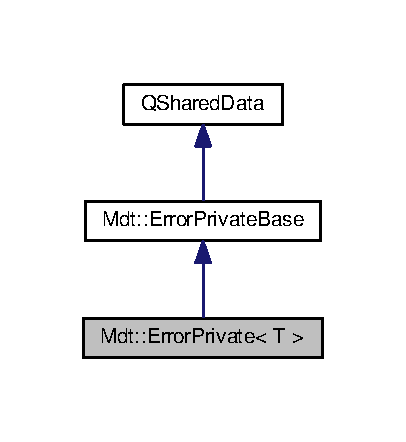
\includegraphics[width=195pt]{struct_mdt_1_1_error_private__inherit__graph}
\end{center}
\end{figure}


Collaboration diagram for Mdt\+:\+:Error\+Private$<$ T $>$\+:
\nopagebreak
\begin{figure}[H]
\begin{center}
\leavevmode
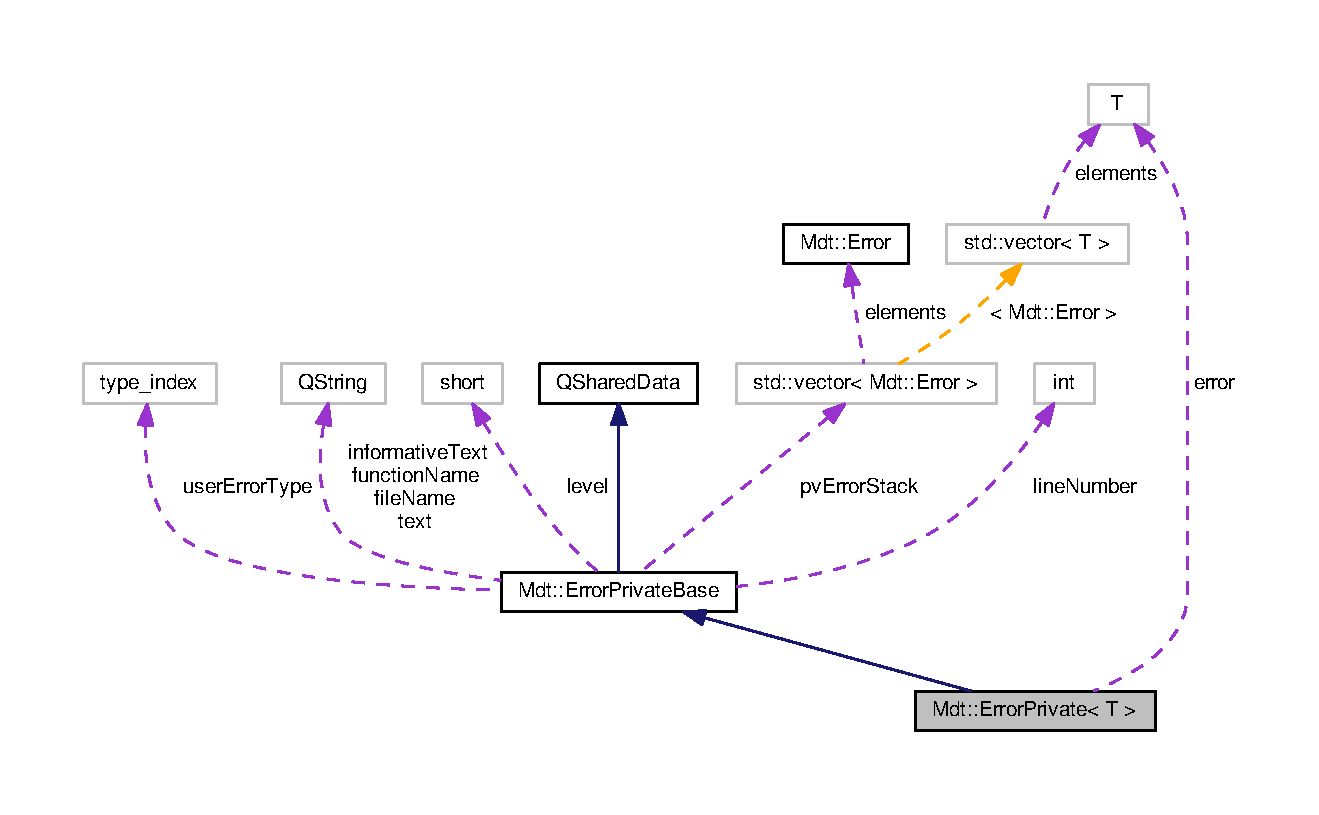
\includegraphics[width=350pt]{struct_mdt_1_1_error_private__coll__graph}
\end{center}
\end{figure}
\subsection*{Public Member Functions}
\begin{DoxyCompactItemize}
\item 
{\bfseries Error\+Private} (const T \&e)\hypertarget{struct_mdt_1_1_error_private_ad9384a0be59f7227352f6b89cd9dadaf}{}\label{struct_mdt_1_1_error_private_ad9384a0be59f7227352f6b89cd9dadaf}

\item 
\hyperlink{struct_mdt_1_1_error_private}{Error\+Private} \& {\bfseries operator=} (const \hyperlink{struct_mdt_1_1_error_private}{Error\+Private} \&)=delete\hypertarget{struct_mdt_1_1_error_private_afacd6a755038d938c5090bbc515aed50}{}\label{struct_mdt_1_1_error_private_afacd6a755038d938c5090bbc515aed50}

\item 
{\bfseries Error\+Private} (\hyperlink{struct_mdt_1_1_error_private}{Error\+Private} \&\&)=delete\hypertarget{struct_mdt_1_1_error_private_aa1a90cbab26f5b7f735274815020879d}{}\label{struct_mdt_1_1_error_private_aa1a90cbab26f5b7f735274815020879d}

\item 
{\bfseries Error\+Private} (const \hyperlink{struct_mdt_1_1_error_private}{Error\+Private} \&other)\hypertarget{struct_mdt_1_1_error_private_a390b87defbbd3bfbcc774dfdbbbdb57d}{}\label{struct_mdt_1_1_error_private_a390b87defbbd3bfbcc774dfdbbbdb57d}

\item 
\hyperlink{struct_mdt_1_1_error_private}{Error\+Private} $\ast$ {\bfseries clone} () const \hypertarget{struct_mdt_1_1_error_private_af7ed703a519fc2216216daaa6dcafb70}{}\label{struct_mdt_1_1_error_private_af7ed703a519fc2216216daaa6dcafb70}

\end{DoxyCompactItemize}
\subsection*{Public Attributes}
\begin{DoxyCompactItemize}
\item 
T {\bfseries error}\hypertarget{struct_mdt_1_1_error_private_a32f76e2ab85a62fe475d39a3276abf3b}{}\label{struct_mdt_1_1_error_private_a32f76e2ab85a62fe475d39a3276abf3b}

\end{DoxyCompactItemize}


\subsection{Detailed Description}
\subsubsection*{template$<$typename T$>$\\*
struct Mdt\+::\+Error\+Private$<$ T $>$}



Definition at line 85 of file Error.\+h.



The documentation for this struct was generated from the following file\+:\begin{DoxyCompactItemize}
\item 
libs/\+Error\+\_\+\+Core/src/\+Mdt/Error.\+h\end{DoxyCompactItemize}

\hypertarget{struct_mdt_1_1_error_private_base}{}\section{Mdt\+:\+:Error\+Private\+Base Struct Reference}
\label{struct_mdt_1_1_error_private_base}\index{Mdt\+::\+Error\+Private\+Base@{Mdt\+::\+Error\+Private\+Base}}


Inheritance diagram for Mdt\+:\+:Error\+Private\+Base\+:\nopagebreak
\begin{figure}[H]
\begin{center}
\leavevmode
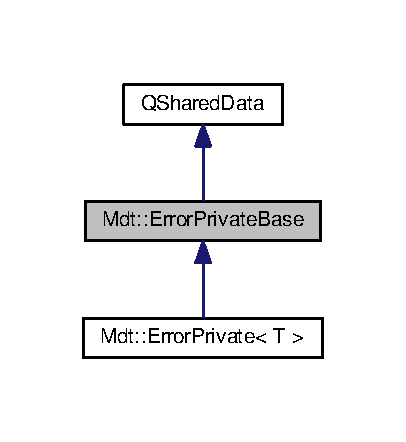
\includegraphics[width=195pt]{struct_mdt_1_1_error_private_base__inherit__graph}
\end{center}
\end{figure}


Collaboration diagram for Mdt\+:\+:Error\+Private\+Base\+:\nopagebreak
\begin{figure}[H]
\begin{center}
\leavevmode
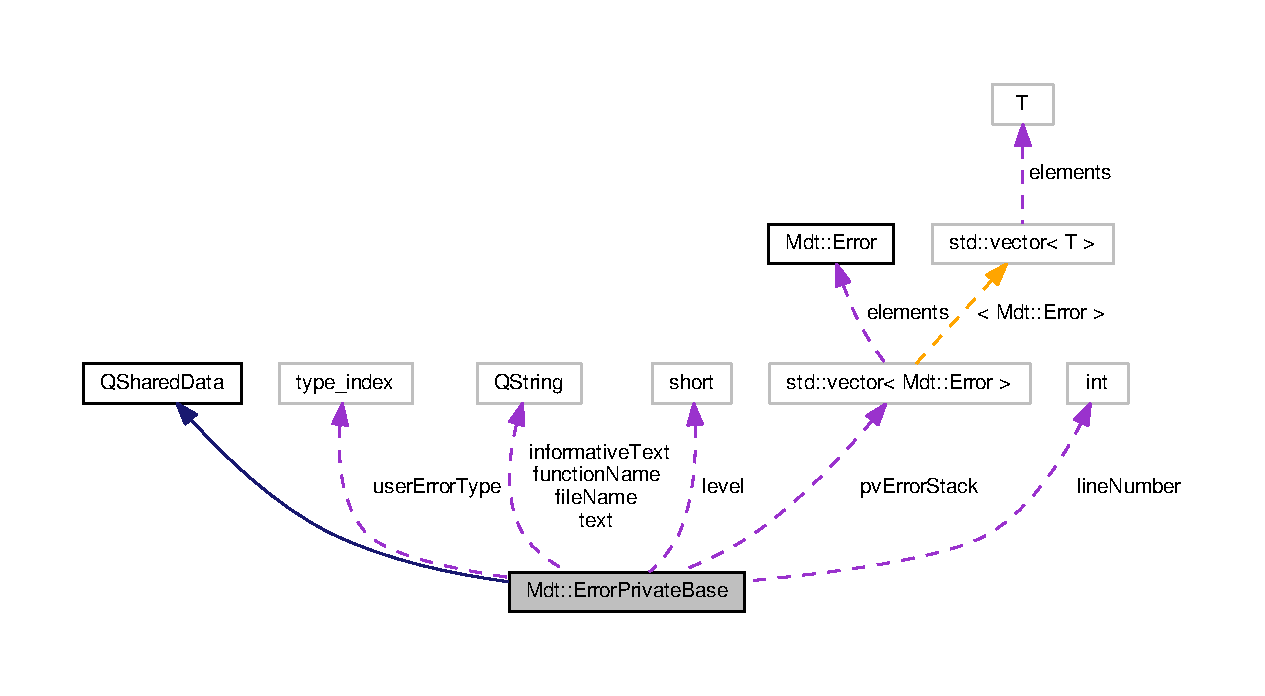
\includegraphics[width=350pt]{struct_mdt_1_1_error_private_base__coll__graph}
\end{center}
\end{figure}
\subsection*{Public Member Functions}
\begin{DoxyCompactItemize}
\item 
\hyperlink{struct_mdt_1_1_error_private_base_a9c56872835666228e16e25c320914b95}{Error\+Private\+Base} (const std\+::type\+\_\+info \&ti)
\begin{DoxyCompactList}\small\item\em Constructor. \end{DoxyCompactList}\item 
{\bfseries Error\+Private\+Base} (const \hyperlink{struct_mdt_1_1_error_private_base}{Error\+Private\+Base} \&other)=default\hypertarget{struct_mdt_1_1_error_private_base_a99e9a3206dbbd651f59cc7a9ac3fafcd}{}\label{struct_mdt_1_1_error_private_base_a99e9a3206dbbd651f59cc7a9ac3fafcd}

\item 
\hyperlink{struct_mdt_1_1_error_private_base}{Error\+Private\+Base} \& {\bfseries operator=} (const \hyperlink{struct_mdt_1_1_error_private_base}{Error\+Private\+Base} \&)=delete\hypertarget{struct_mdt_1_1_error_private_base_a42d145fc08ca241cdaafec1ef16d52df}{}\label{struct_mdt_1_1_error_private_base_a42d145fc08ca241cdaafec1ef16d52df}

\item 
{\bfseries Error\+Private\+Base} (\hyperlink{struct_mdt_1_1_error_private_base}{Error\+Private\+Base} \&\&)=delete\hypertarget{struct_mdt_1_1_error_private_base_ad1f98f8d45b815858425423ad4108e35}{}\label{struct_mdt_1_1_error_private_base_ad1f98f8d45b815858425423ad4108e35}

\item 
virtual \hyperlink{struct_mdt_1_1_error_private_base}{Error\+Private\+Base} $\ast$ {\bfseries clone} () const =0\hypertarget{struct_mdt_1_1_error_private_base_afca32564ec7cae7463e8e23560d0917d}{}\label{struct_mdt_1_1_error_private_base_afca32564ec7cae7463e8e23560d0917d}

\end{DoxyCompactItemize}
\subsection*{Public Attributes}
\begin{DoxyCompactItemize}
\item 
short {\bfseries level}\hypertarget{struct_mdt_1_1_error_private_base_afe6b790268a89f523343d45451433b6e}{}\label{struct_mdt_1_1_error_private_base_afe6b790268a89f523343d45451433b6e}

\item 
std\+::type\+\_\+index {\bfseries user\+Error\+Type}\hypertarget{struct_mdt_1_1_error_private_base_a236cc35b1b54ab87b925000822b6bdba}{}\label{struct_mdt_1_1_error_private_base_a236cc35b1b54ab87b925000822b6bdba}

\item 
Q\+String {\bfseries text}\hypertarget{struct_mdt_1_1_error_private_base_afdc8351f73b50f94ef0b8778356eecf3}{}\label{struct_mdt_1_1_error_private_base_afdc8351f73b50f94ef0b8778356eecf3}

\item 
Q\+String {\bfseries informative\+Text}\hypertarget{struct_mdt_1_1_error_private_base_af41153fe6f24b341540e278bbfff4453}{}\label{struct_mdt_1_1_error_private_base_af41153fe6f24b341540e278bbfff4453}

\item 
std\+::vector$<$ \hyperlink{class_mdt_1_1_error}{Error} $>$ {\bfseries pv\+Error\+Stack}\hypertarget{struct_mdt_1_1_error_private_base_a9948c2d1794611121634facecb878d53}{}\label{struct_mdt_1_1_error_private_base_a9948c2d1794611121634facecb878d53}

\item 
Q\+String {\bfseries file\+Name}\hypertarget{struct_mdt_1_1_error_private_base_af1b038461d8c99b72bf19478873d7584}{}\label{struct_mdt_1_1_error_private_base_af1b038461d8c99b72bf19478873d7584}

\item 
int {\bfseries line\+Number}\hypertarget{struct_mdt_1_1_error_private_base_a4bbfc69740ea1d2de4c2025956507e37}{}\label{struct_mdt_1_1_error_private_base_a4bbfc69740ea1d2de4c2025956507e37}

\item 
Q\+String {\bfseries function\+Name}\hypertarget{struct_mdt_1_1_error_private_base_a6b0b69143256b553ee00f0a72ad52edb}{}\label{struct_mdt_1_1_error_private_base_a6b0b69143256b553ee00f0a72ad52edb}

\end{DoxyCompactItemize}


\subsection{Detailed Description}


Definition at line 48 of file Error.\+h.



\subsection{Constructor \& Destructor Documentation}
\index{Mdt\+::\+Error\+Private\+Base@{Mdt\+::\+Error\+Private\+Base}!Error\+Private\+Base@{Error\+Private\+Base}}
\index{Error\+Private\+Base@{Error\+Private\+Base}!Mdt\+::\+Error\+Private\+Base@{Mdt\+::\+Error\+Private\+Base}}
\subsubsection[{\texorpdfstring{Error\+Private\+Base(const std\+::type\+\_\+info \&ti)}{ErrorPrivateBase(const std::type_info &ti)}}]{\setlength{\rightskip}{0pt plus 5cm}Mdt\+::\+Error\+Private\+Base\+::\+Error\+Private\+Base (
\begin{DoxyParamCaption}
\item[{const std\+::type\+\_\+info \&}]{ti}
\end{DoxyParamCaption}
)\hspace{0.3cm}{\ttfamily [inline]}}\hypertarget{struct_mdt_1_1_error_private_base_a9c56872835666228e16e25c320914b95}{}\label{struct_mdt_1_1_error_private_base_a9c56872835666228e16e25c320914b95}


Constructor. 



Definition at line 52 of file Error.\+h.



The documentation for this struct was generated from the following file\+:\begin{DoxyCompactItemize}
\item 
libs/\+Error\+\_\+\+Core/src/\+Mdt/Error.\+h\end{DoxyCompactItemize}

\hypertarget{class_mdt_1_1_error_q_process}{}\section{Mdt\+:\+:Error\+Q\+Process Class Reference}
\label{class_mdt_1_1_error_q_process}\index{Mdt\+::\+Error\+Q\+Process@{Mdt\+::\+Error\+Q\+Process}}


Translate Q\+Process errors to \hyperlink{class_mdt_1_1_error}{Mdt\+::\+Error}.  




{\ttfamily \#include $<$Error\+Q\+Process.\+h$>$}

\subsection*{Static Public Member Functions}
\begin{DoxyCompactItemize}
\item 
static \hyperlink{class_mdt_1_1_error}{Mdt\+::\+Error} \hyperlink{class_mdt_1_1_error_q_process_a2dda98dd359be476ce2039c5a5a9c157}{from\+Q\+Process} (const Q\+Process \&process, const Q\+String \&file, int line, const Q\+String \&class\+Name, const Q\+String \&function\+Name)
\begin{DoxyCompactList}\small\item\em Get a \hyperlink{class_mdt_1_1_error}{Mdt\+::\+Error} from last error in {\itshape process}. \end{DoxyCompactList}\item 
static \hyperlink{class_mdt_1_1_error}{Mdt\+::\+Error} \hyperlink{class_mdt_1_1_error_q_process_a013ef5e5f23c26375845ef9e925adef3}{from\+Q\+Process} (const Q\+Process \&process, const Q\+String \&file, int line, const Q\+Object $\ast$const obj, const Q\+String \&function\+Name)
\begin{DoxyCompactList}\small\item\em Get a \hyperlink{class_mdt_1_1_error}{Mdt\+::\+Error} from last error in {\itshape process}. \end{DoxyCompactList}\end{DoxyCompactItemize}


\subsection{Detailed Description}
Translate Q\+Process errors to \hyperlink{class_mdt_1_1_error}{Mdt\+::\+Error}. 

\begin{DoxySeeAlso}{See also}
mdt\+Error\+From\+Q\+Process() 

mdt\+Error\+From\+Q\+Process\+Q() 
\end{DoxySeeAlso}


Definition at line 54 of file Error\+Q\+Process.\+h.



\subsection{Member Function Documentation}
\index{Mdt\+::\+Error\+Q\+Process@{Mdt\+::\+Error\+Q\+Process}!from\+Q\+Process@{from\+Q\+Process}}
\index{from\+Q\+Process@{from\+Q\+Process}!Mdt\+::\+Error\+Q\+Process@{Mdt\+::\+Error\+Q\+Process}}
\subsubsection[{\texorpdfstring{from\+Q\+Process(const Q\+Process \&process, const Q\+String \&file, int line, const Q\+String \&class\+Name, const Q\+String \&function\+Name)}{fromQProcess(const QProcess &process, const QString &file, int line, const QString &className, const QString &functionName)}}]{\setlength{\rightskip}{0pt plus 5cm}{\bf Error} Mdt\+::\+Error\+Q\+Process\+::from\+Q\+Process (
\begin{DoxyParamCaption}
\item[{const Q\+Process \&}]{process, }
\item[{const Q\+String \&}]{file, }
\item[{int}]{line, }
\item[{const Q\+String \&}]{class\+Name, }
\item[{const Q\+String \&}]{function\+Name}
\end{DoxyParamCaption}
)\hspace{0.3cm}{\ttfamily [static]}}\hypertarget{class_mdt_1_1_error_q_process_a2dda98dd359be476ce2039c5a5a9c157}{}\label{class_mdt_1_1_error_q_process_a2dda98dd359be476ce2039c5a5a9c157}


Get a \hyperlink{class_mdt_1_1_error}{Mdt\+::\+Error} from last error in {\itshape process}. 

\begin{DoxySeeAlso}{See also}
mdt\+Error\+From\+Q\+Process() 
\end{DoxySeeAlso}


Definition at line 44 of file Error\+Q\+Process.\+cpp.

\index{Mdt\+::\+Error\+Q\+Process@{Mdt\+::\+Error\+Q\+Process}!from\+Q\+Process@{from\+Q\+Process}}
\index{from\+Q\+Process@{from\+Q\+Process}!Mdt\+::\+Error\+Q\+Process@{Mdt\+::\+Error\+Q\+Process}}
\subsubsection[{\texorpdfstring{from\+Q\+Process(const Q\+Process \&process, const Q\+String \&file, int line, const Q\+Object $\ast$const obj, const Q\+String \&function\+Name)}{fromQProcess(const QProcess &process, const QString &file, int line, const QObject *const obj, const QString &functionName)}}]{\setlength{\rightskip}{0pt plus 5cm}{\bf Error} Mdt\+::\+Error\+Q\+Process\+::from\+Q\+Process (
\begin{DoxyParamCaption}
\item[{const Q\+Process \&}]{process, }
\item[{const Q\+String \&}]{file, }
\item[{int}]{line, }
\item[{const Q\+Object $\ast$const}]{obj, }
\item[{const Q\+String \&}]{function\+Name}
\end{DoxyParamCaption}
)\hspace{0.3cm}{\ttfamily [static]}}\hypertarget{class_mdt_1_1_error_q_process_a013ef5e5f23c26375845ef9e925adef3}{}\label{class_mdt_1_1_error_q_process_a013ef5e5f23c26375845ef9e925adef3}


Get a \hyperlink{class_mdt_1_1_error}{Mdt\+::\+Error} from last error in {\itshape process}. 

\begin{DoxySeeAlso}{See also}
mdt\+Error\+From\+Q\+Process\+Q() 
\end{DoxySeeAlso}


Definition at line 55 of file Error\+Q\+Process.\+cpp.



The documentation for this class was generated from the following files\+:\begin{DoxyCompactItemize}
\item 
libs/\+Error\+\_\+\+Core/src/\+Mdt/Error\+Q\+Process.\+h\item 
libs/\+Error\+\_\+\+Core/src/\+Mdt/Error\+Q\+Process.\+cpp\end{DoxyCompactItemize}

\hypertarget{class_mdt_1_1_error_logger_1_1_file_backend}{}\section{Mdt\+:\+:Error\+Logger\+:\+:File\+Backend Class Reference}
\label{class_mdt_1_1_error_logger_1_1_file_backend}\index{Mdt\+::\+Error\+Logger\+::\+File\+Backend@{Mdt\+::\+Error\+Logger\+::\+File\+Backend}}


File backend for error \hyperlink{class_mdt_1_1_error_logger_1_1_logger}{Logger}.  




{\ttfamily \#include $<$File\+Backend.\+h$>$}



Inheritance diagram for Mdt\+:\+:Error\+Logger\+:\+:File\+Backend\+:\nopagebreak
\begin{figure}[H]
\begin{center}
\leavevmode
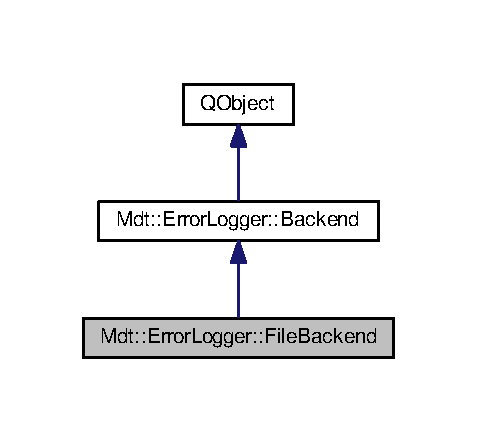
\includegraphics[width=229pt]{class_mdt_1_1_error_logger_1_1_file_backend__inherit__graph}
\end{center}
\end{figure}


Collaboration diagram for Mdt\+:\+:Error\+Logger\+:\+:File\+Backend\+:\nopagebreak
\begin{figure}[H]
\begin{center}
\leavevmode
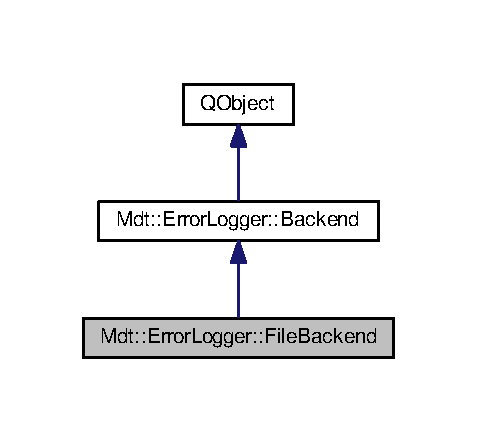
\includegraphics[width=229pt]{class_mdt_1_1_error_logger_1_1_file_backend__coll__graph}
\end{center}
\end{figure}
\subsection*{Public Member Functions}
\begin{DoxyCompactItemize}
\item 
\hyperlink{class_mdt_1_1_error_logger_1_1_file_backend_a8587ac2a6cd89416878b389138e79a3a}{File\+Backend} ()
\begin{DoxyCompactList}\small\item\em Constructor. \end{DoxyCompactList}\item 
\hyperlink{class_mdt_1_1_error_logger_1_1_file_backend_a5f7262e481d756d7145bbfa42aeca91e}{$\sim$\+File\+Backend} ()
\begin{DoxyCompactList}\small\item\em Destructor. \end{DoxyCompactList}\item 
bool \hyperlink{class_mdt_1_1_error_logger_1_1_file_backend_a844fc6f89a147b0713700028808e364a}{set\+Log\+File\+Path} (const Q\+String \&path, qint64 \hyperlink{class_mdt_1_1_error_logger_1_1_file_backend_a8c5943cdd59ed5941c72490d7b414359}{max\+File\+Size}=1024 $\ast$1024)
\begin{DoxyCompactList}\small\item\em Set path to log file. \end{DoxyCompactList}\item 
Q\+String \hyperlink{class_mdt_1_1_error_logger_1_1_file_backend_ac25cd41dbbe940bf0247e5054ce8805e}{log\+File\+Path} () const 
\begin{DoxyCompactList}\small\item\em Get log file path. \end{DoxyCompactList}\item 
Q\+String \hyperlink{class_mdt_1_1_error_logger_1_1_file_backend_a7c79c940be2f03f22111638d2e749a64}{backup\+Log\+File\+Path} () const 
\begin{DoxyCompactList}\small\item\em Get backup log file path. \end{DoxyCompactList}\item 
qint64 \hyperlink{class_mdt_1_1_error_logger_1_1_file_backend_a8c5943cdd59ed5941c72490d7b414359}{max\+File\+Size} () const 
\begin{DoxyCompactList}\small\item\em Get maximum log file size. \end{DoxyCompactList}\item 
void \hyperlink{class_mdt_1_1_error_logger_1_1_file_backend_a31b8314d523a491b5441276122daed87}{log\+Error} (const \hyperlink{class_mdt_1_1_error}{Error} \&error)
\begin{DoxyCompactList}\small\item\em Log given error. \end{DoxyCompactList}\end{DoxyCompactItemize}
\subsection*{Additional Inherited Members}


\subsection{Detailed Description}
File backend for error \hyperlink{class_mdt_1_1_error_logger_1_1_logger}{Logger}. 

Definition at line 34 of file File\+Backend.\+h.



\subsection{Constructor \& Destructor Documentation}
\index{Mdt\+::\+Error\+Logger\+::\+File\+Backend@{Mdt\+::\+Error\+Logger\+::\+File\+Backend}!File\+Backend@{File\+Backend}}
\index{File\+Backend@{File\+Backend}!Mdt\+::\+Error\+Logger\+::\+File\+Backend@{Mdt\+::\+Error\+Logger\+::\+File\+Backend}}
\subsubsection[{\texorpdfstring{File\+Backend()}{FileBackend()}}]{\setlength{\rightskip}{0pt plus 5cm}Mdt\+::\+Error\+Logger\+::\+File\+Backend\+::\+File\+Backend (
\begin{DoxyParamCaption}
{}
\end{DoxyParamCaption}
)}\hypertarget{class_mdt_1_1_error_logger_1_1_file_backend_a8587ac2a6cd89416878b389138e79a3a}{}\label{class_mdt_1_1_error_logger_1_1_file_backend_a8587ac2a6cd89416878b389138e79a3a}


Constructor. 



Definition at line 32 of file File\+Backend.\+cpp.

\index{Mdt\+::\+Error\+Logger\+::\+File\+Backend@{Mdt\+::\+Error\+Logger\+::\+File\+Backend}!````~File\+Backend@{$\sim$\+File\+Backend}}
\index{````~File\+Backend@{$\sim$\+File\+Backend}!Mdt\+::\+Error\+Logger\+::\+File\+Backend@{Mdt\+::\+Error\+Logger\+::\+File\+Backend}}
\subsubsection[{\texorpdfstring{$\sim$\+File\+Backend()}{~FileBackend()}}]{\setlength{\rightskip}{0pt plus 5cm}Mdt\+::\+Error\+Logger\+::\+File\+Backend\+::$\sim$\+File\+Backend (
\begin{DoxyParamCaption}
{}
\end{DoxyParamCaption}
)}\hypertarget{class_mdt_1_1_error_logger_1_1_file_backend_a5f7262e481d756d7145bbfa42aeca91e}{}\label{class_mdt_1_1_error_logger_1_1_file_backend_a5f7262e481d756d7145bbfa42aeca91e}


Destructor. 



Definition at line 37 of file File\+Backend.\+cpp.



\subsection{Member Function Documentation}
\index{Mdt\+::\+Error\+Logger\+::\+File\+Backend@{Mdt\+::\+Error\+Logger\+::\+File\+Backend}!backup\+Log\+File\+Path@{backup\+Log\+File\+Path}}
\index{backup\+Log\+File\+Path@{backup\+Log\+File\+Path}!Mdt\+::\+Error\+Logger\+::\+File\+Backend@{Mdt\+::\+Error\+Logger\+::\+File\+Backend}}
\subsubsection[{\texorpdfstring{backup\+Log\+File\+Path() const }{backupLogFilePath() const }}]{\setlength{\rightskip}{0pt plus 5cm}Q\+String Mdt\+::\+Error\+Logger\+::\+File\+Backend\+::backup\+Log\+File\+Path (
\begin{DoxyParamCaption}
{}
\end{DoxyParamCaption}
) const}\hypertarget{class_mdt_1_1_error_logger_1_1_file_backend_a7c79c940be2f03f22111638d2e749a64}{}\label{class_mdt_1_1_error_logger_1_1_file_backend_a7c79c940be2f03f22111638d2e749a64}


Get backup log file path. 



Definition at line 64 of file File\+Backend.\+cpp.

\index{Mdt\+::\+Error\+Logger\+::\+File\+Backend@{Mdt\+::\+Error\+Logger\+::\+File\+Backend}!log\+Error@{log\+Error}}
\index{log\+Error@{log\+Error}!Mdt\+::\+Error\+Logger\+::\+File\+Backend@{Mdt\+::\+Error\+Logger\+::\+File\+Backend}}
\subsubsection[{\texorpdfstring{log\+Error(const Error \&error)}{logError(const Error &error)}}]{\setlength{\rightskip}{0pt plus 5cm}void Mdt\+::\+Error\+Logger\+::\+File\+Backend\+::log\+Error (
\begin{DoxyParamCaption}
\item[{const {\bf Error} \&}]{error}
\end{DoxyParamCaption}
)\hspace{0.3cm}{\ttfamily [virtual]}}\hypertarget{class_mdt_1_1_error_logger_1_1_file_backend_a31b8314d523a491b5441276122daed87}{}\label{class_mdt_1_1_error_logger_1_1_file_backend_a31b8314d523a491b5441276122daed87}


Log given error. 



Implements \hyperlink{class_mdt_1_1_error_logger_1_1_backend_acf37cfc576269934ca8ce04e3601058d}{Mdt\+::\+Error\+Logger\+::\+Backend}.



Definition at line 74 of file File\+Backend.\+cpp.

\index{Mdt\+::\+Error\+Logger\+::\+File\+Backend@{Mdt\+::\+Error\+Logger\+::\+File\+Backend}!log\+File\+Path@{log\+File\+Path}}
\index{log\+File\+Path@{log\+File\+Path}!Mdt\+::\+Error\+Logger\+::\+File\+Backend@{Mdt\+::\+Error\+Logger\+::\+File\+Backend}}
\subsubsection[{\texorpdfstring{log\+File\+Path() const }{logFilePath() const }}]{\setlength{\rightskip}{0pt plus 5cm}Q\+String Mdt\+::\+Error\+Logger\+::\+File\+Backend\+::log\+File\+Path (
\begin{DoxyParamCaption}
{}
\end{DoxyParamCaption}
) const}\hypertarget{class_mdt_1_1_error_logger_1_1_file_backend_ac25cd41dbbe940bf0247e5054ce8805e}{}\label{class_mdt_1_1_error_logger_1_1_file_backend_ac25cd41dbbe940bf0247e5054ce8805e}


Get log file path. 



Definition at line 59 of file File\+Backend.\+cpp.

\index{Mdt\+::\+Error\+Logger\+::\+File\+Backend@{Mdt\+::\+Error\+Logger\+::\+File\+Backend}!max\+File\+Size@{max\+File\+Size}}
\index{max\+File\+Size@{max\+File\+Size}!Mdt\+::\+Error\+Logger\+::\+File\+Backend@{Mdt\+::\+Error\+Logger\+::\+File\+Backend}}
\subsubsection[{\texorpdfstring{max\+File\+Size() const }{maxFileSize() const }}]{\setlength{\rightskip}{0pt plus 5cm}qint64 Mdt\+::\+Error\+Logger\+::\+File\+Backend\+::max\+File\+Size (
\begin{DoxyParamCaption}
{}
\end{DoxyParamCaption}
) const}\hypertarget{class_mdt_1_1_error_logger_1_1_file_backend_a8c5943cdd59ed5941c72490d7b414359}{}\label{class_mdt_1_1_error_logger_1_1_file_backend_a8c5943cdd59ed5941c72490d7b414359}


Get maximum log file size. 



Definition at line 69 of file File\+Backend.\+cpp.

\index{Mdt\+::\+Error\+Logger\+::\+File\+Backend@{Mdt\+::\+Error\+Logger\+::\+File\+Backend}!set\+Log\+File\+Path@{set\+Log\+File\+Path}}
\index{set\+Log\+File\+Path@{set\+Log\+File\+Path}!Mdt\+::\+Error\+Logger\+::\+File\+Backend@{Mdt\+::\+Error\+Logger\+::\+File\+Backend}}
\subsubsection[{\texorpdfstring{set\+Log\+File\+Path(const Q\+String \&path, qint64 max\+File\+Size=1024 $\ast$1024)}{setLogFilePath(const QString &path, qint64 maxFileSize=1024 *1024)}}]{\setlength{\rightskip}{0pt plus 5cm}bool Mdt\+::\+Error\+Logger\+::\+File\+Backend\+::set\+Log\+File\+Path (
\begin{DoxyParamCaption}
\item[{const Q\+String \&}]{path, }
\item[{qint64}]{max\+File\+Size = {\ttfamily 1024$\ast$1024}}
\end{DoxyParamCaption}
)}\hypertarget{class_mdt_1_1_error_logger_1_1_file_backend_a844fc6f89a147b0713700028808e364a}{}\label{class_mdt_1_1_error_logger_1_1_file_backend_a844fc6f89a147b0713700028808e364a}


Set path to log file. 


\begin{DoxyParams}{Parameters}
{\em path} & Path to the log file. Note that a backup is made in same directory than file given by path, with a other exention. \\
\hline
{\em max\+File\+Size} & Maximum size allowed for log file \mbox{[}Byte\mbox{]} Also note that the file can be some bytes greater than specified size. \\
\hline
\end{DoxyParams}
\begin{DoxyNote}{Note}
This function should only be called before this Logger\+File\+Backend is passed to the \hyperlink{class_mdt_1_1_error_logger_1_1_logger}{Logger} (changing file path while \hyperlink{class_mdt_1_1_error_logger_1_1_logger}{Logger} is calling \hyperlink{class_mdt_1_1_error_logger_1_1_file_backend_a31b8314d523a491b5441276122daed87}{log\+Error()} is undefined behaviour). 
\end{DoxyNote}


Definition at line 41 of file File\+Backend.\+cpp.



The documentation for this class was generated from the following files\+:\begin{DoxyCompactItemize}
\item 
libs/\+Error\+\_\+\+Core/src/\+Mdt/\+Error\+Logger/File\+Backend.\+h\item 
libs/\+Error\+\_\+\+Core/src/\+Mdt/\+Error\+Logger/File\+Backend.\+cpp\end{DoxyCompactItemize}

\hypertarget{struct_mdt_1_1_generic_error}{}\section{Mdt\+:\+:Generic\+Error Struct Reference}
\label{struct_mdt_1_1_generic_error}\index{Mdt\+::\+Generic\+Error@{Mdt\+::\+Generic\+Error}}


\subsection{Detailed Description}


Definition at line 42 of file Error.\+h.



The documentation for this struct was generated from the following file\+:\begin{DoxyCompactItemize}
\item 
libs/\+Error\+\_\+\+Core/src/\+Mdt/Error.\+h\end{DoxyCompactItemize}

\hypertarget{class_mdt_1_1_error_logger_1_1_logger}{}\section{Mdt\+:\+:Error\+Logger\+:\+:Logger Class Reference}
\label{class_mdt_1_1_error_logger_1_1_logger}\index{Mdt\+::\+Error\+Logger\+::\+Logger@{Mdt\+::\+Error\+Logger\+::\+Logger}}


Helper class to log \hyperlink{class_mdt_1_1_error}{Error} objects.  




{\ttfamily \#include $<$Logger.\+h$>$}



Inherits Q\+Object.

\subsection*{Public Types}
\subsection*{Static Public Member Functions}
\begin{DoxyCompactItemize}
\item 
{\footnotesize template$<$typename T $>$ }\\static T $\ast$ \hyperlink{class_mdt_1_1_error_logger_1_1_logger_ae011d85c251d55660c3f90f21d1ab2a6}{add\+Backend} (\hyperlink{class_mdt_1_1_error_logger_1_1_logger_ab6d6198b43b2bb94cede114ec67b781c}{Execution\+Thread} execution\+Thread)
\begin{DoxyCompactList}\small\item\em Add a logger backend. \end{DoxyCompactList}\item 
static void \hyperlink{class_mdt_1_1_error_logger_1_1_logger_aa06a24a1d521258729ca172465b02040}{log\+Error} (const \hyperlink{class_mdt_1_1_error}{Error} \&error)
\begin{DoxyCompactList}\small\item\em Log given error. \end{DoxyCompactList}\item 
static void \hyperlink{class_mdt_1_1_error_logger_1_1_logger_a3bb1951ee52da826fde82dab52d54c4b}{cleanup} ()
\begin{DoxyCompactList}\small\item\em Cleanup. \end{DoxyCompactList}\end{DoxyCompactItemize}


\subsection{Detailed Description}
Helper class to log \hyperlink{class_mdt_1_1_error}{Error} objects. 

Definition at line 41 of file Logger.\+h.



\subsection{Member Enumeration Documentation}
\index{Mdt\+::\+Error\+Logger\+::\+Logger@{Mdt\+::\+Error\+Logger\+::\+Logger}!Execution\+Thread@{Execution\+Thread}}
\index{Execution\+Thread@{Execution\+Thread}!Mdt\+::\+Error\+Logger\+::\+Logger@{Mdt\+::\+Error\+Logger\+::\+Logger}}
\subsubsection[{\texorpdfstring{Execution\+Thread}{ExecutionThread}}]{\setlength{\rightskip}{0pt plus 5cm}enum {\bf Mdt\+::\+Error\+Logger\+::\+Logger\+::\+Execution\+Thread}}\hypertarget{class_mdt_1_1_error_logger_1_1_logger_ab6d6198b43b2bb94cede114ec67b781c}{}\label{class_mdt_1_1_error_logger_1_1_logger_ab6d6198b43b2bb94cede114ec67b781c}


Execution thread of a backend. 

When adding a backend to the logger, it is possible to choose in which thread it must run. \begin{Desc}
\item[Enumerator]\par
\begin{description}
\index{Execute\+In\+Main\+Thread@{Execute\+In\+Main\+Thread}!Mdt\+::\+Error\+Logger\+::\+Logger@{Mdt\+::\+Error\+Logger\+::\+Logger}}\index{Mdt\+::\+Error\+Logger\+::\+Logger@{Mdt\+::\+Error\+Logger\+::\+Logger}!Execute\+In\+Main\+Thread@{Execute\+In\+Main\+Thread}}\item[{\em 
Execute\+In\+Main\+Thread\hypertarget{class_mdt_1_1_error_logger_1_1_logger_ab6d6198b43b2bb94cede114ec67b781caac54433e68e1f766627c9fcc87f7b818}{}\label{class_mdt_1_1_error_logger_1_1_logger_ab6d6198b43b2bb94cede114ec67b781caac54433e68e1f766627c9fcc87f7b818}
}]The backend will run in the main thread. The Qt\textquotesingle{}s signal/slot is used with a auto connection, so that errors logged using \hyperlink{class_mdt_1_1_error_logger_1_1_logger_aa06a24a1d521258729ca172465b02040}{log\+Error()} will allways call \hyperlink{class_mdt_1_1_error_logger_1_1_backend_acf37cfc576269934ca8ce04e3601058d}{Backend\+::log\+Error()} from the main thread event loop, regardless of the caller thread. \index{Execute\+In\+Separate\+Thread@{Execute\+In\+Separate\+Thread}!Mdt\+::\+Error\+Logger\+::\+Logger@{Mdt\+::\+Error\+Logger\+::\+Logger}}\index{Mdt\+::\+Error\+Logger\+::\+Logger@{Mdt\+::\+Error\+Logger\+::\+Logger}!Execute\+In\+Separate\+Thread@{Execute\+In\+Separate\+Thread}}\item[{\em 
Execute\+In\+Separate\+Thread\hypertarget{class_mdt_1_1_error_logger_1_1_logger_ab6d6198b43b2bb94cede114ec67b781caf7dfdc36418cac0a65cea2cde2a11fd7}{}\label{class_mdt_1_1_error_logger_1_1_logger_ab6d6198b43b2bb94cede114ec67b781caf7dfdc36418cac0a65cea2cde2a11fd7}
}]The backend will run in logger\textquotesingle{}s separate thread. A call to \hyperlink{class_mdt_1_1_error_logger_1_1_logger_aa06a24a1d521258729ca172465b02040}{log\+Error()} will allways just queue the error and return. The logger\textquotesingle{}s separated thread will then call \hyperlink{class_mdt_1_1_error_logger_1_1_backend_acf37cfc576269934ca8ce04e3601058d}{Backend\+::log\+Error()}. \end{description}
\end{Desc}


Definition at line 53 of file Logger.\+h.



\subsection{Member Function Documentation}
\index{Mdt\+::\+Error\+Logger\+::\+Logger@{Mdt\+::\+Error\+Logger\+::\+Logger}!add\+Backend@{add\+Backend}}
\index{add\+Backend@{add\+Backend}!Mdt\+::\+Error\+Logger\+::\+Logger@{Mdt\+::\+Error\+Logger\+::\+Logger}}
\subsubsection[{\texorpdfstring{add\+Backend(\+Execution\+Thread execution\+Thread)}{addBackend(ExecutionThread executionThread)}}]{\setlength{\rightskip}{0pt plus 5cm}template$<$typename T $>$ static T$\ast$ Mdt\+::\+Error\+Logger\+::\+Logger\+::add\+Backend (
\begin{DoxyParamCaption}
\item[{{\bf Execution\+Thread}}]{execution\+Thread}
\end{DoxyParamCaption}
)\hspace{0.3cm}{\ttfamily [inline]}, {\ttfamily [static]}}\hypertarget{class_mdt_1_1_error_logger_1_1_logger_ae011d85c251d55660c3f90f21d1ab2a6}{}\label{class_mdt_1_1_error_logger_1_1_logger_ae011d85c251d55660c3f90f21d1ab2a6}


Add a logger backend. 


\begin{DoxyCode}
\textcolor{keyword}{using} \hyperlink{class_mdt_1_1_error_logger_1_1_logger}{Mdt::ErrorLogger::Logger};

\textcolor{keyword}{auto} backend = Logger::addBackend<FileBackend>(\hyperlink{class_mdt_1_1_error_logger_1_1_logger_ab6d6198b43b2bb94cede114ec67b781caf7dfdc36418cac0a65cea2cde2a11fd7}{Logger::ExecuteInSeparateThread}
      );
backend->setLogFilePath(\textcolor{stringliteral}{"some/path/to/logfile"});
\end{DoxyCode}


A backend of type T is instanciated and added to the list of backends runing on specified {\itshape execution\+Thread} . A pointer to the created backend is returned, so that some setup can be done on the backend. The logger has the ownership of the backend (it will delete it).

Accessing the backend referenced by the returned pointer is only possible\+:
\begin{DoxyItemize}
\item If it runs on separate thread, before any error is logged ( by calling \hyperlink{class_mdt_1_1_error_logger_1_1_logger_aa06a24a1d521258729ca172465b02040}{log\+Error()} )
\item For all cases, before calling \hyperlink{class_mdt_1_1_error_logger_1_1_logger_a3bb1951ee52da826fde82dab52d54c4b}{cleanup()} 
\end{DoxyItemize}

Definition at line 94 of file Logger.\+h.

\index{Mdt\+::\+Error\+Logger\+::\+Logger@{Mdt\+::\+Error\+Logger\+::\+Logger}!cleanup@{cleanup}}
\index{cleanup@{cleanup}!Mdt\+::\+Error\+Logger\+::\+Logger@{Mdt\+::\+Error\+Logger\+::\+Logger}}
\subsubsection[{\texorpdfstring{cleanup()}{cleanup()}}]{\setlength{\rightskip}{0pt plus 5cm}void Mdt\+::\+Error\+Logger\+::\+Logger\+::cleanup (
\begin{DoxyParamCaption}
{}
\end{DoxyParamCaption}
)\hspace{0.3cm}{\ttfamily [static]}}\hypertarget{class_mdt_1_1_error_logger_1_1_logger_a3bb1951ee52da826fde82dab52d54c4b}{}\label{class_mdt_1_1_error_logger_1_1_logger_a3bb1951ee52da826fde82dab52d54c4b}


Cleanup. 

\begin{DoxyNote}{Note}
This function must be called before returning from main(). Not doing so conducts to undefined behaviour. Consider using a \hyperlink{class_mdt_1_1_error_logger_1_1_logger_guard}{Logger\+Guard}. 
\end{DoxyNote}


Definition at line 36 of file Logger.\+cpp.

\index{Mdt\+::\+Error\+Logger\+::\+Logger@{Mdt\+::\+Error\+Logger\+::\+Logger}!log\+Error@{log\+Error}}
\index{log\+Error@{log\+Error}!Mdt\+::\+Error\+Logger\+::\+Logger@{Mdt\+::\+Error\+Logger\+::\+Logger}}
\subsubsection[{\texorpdfstring{log\+Error(const Error \&error)}{logError(const Error &error)}}]{\setlength{\rightskip}{0pt plus 5cm}void Mdt\+::\+Error\+Logger\+::\+Logger\+::log\+Error (
\begin{DoxyParamCaption}
\item[{const {\bf Error} \&}]{error}
\end{DoxyParamCaption}
)\hspace{0.3cm}{\ttfamily [static]}}\hypertarget{class_mdt_1_1_error_logger_1_1_logger_aa06a24a1d521258729ca172465b02040}{}\label{class_mdt_1_1_error_logger_1_1_logger_aa06a24a1d521258729ca172465b02040}


Log given error. 

This function is thread safe

\begin{DoxyPrecond}{Precondition}
{\itshape error} must not be null 
\end{DoxyPrecond}


Definition at line 28 of file Logger.\+cpp.



The documentation for this class was generated from the following files\+:\begin{DoxyCompactItemize}
\item 
libs/\+Error\+\_\+\+Core/src/\+Mdt/\+Error\+Logger/Logger.\+h\item 
libs/\+Error\+\_\+\+Core/src/\+Mdt/\+Error\+Logger/Logger.\+cpp\end{DoxyCompactItemize}

\hypertarget{class_mdt_1_1_error_logger_1_1_logger_guard}{}\section{Mdt\+:\+:Error\+Logger\+:\+:Logger\+Guard Class Reference}
\label{class_mdt_1_1_error_logger_1_1_logger_guard}\index{Mdt\+::\+Error\+Logger\+::\+Logger\+Guard@{Mdt\+::\+Error\+Logger\+::\+Logger\+Guard}}


Scope guard for error \hyperlink{class_mdt_1_1_error_logger_1_1_logger}{Logger}.  




{\ttfamily \#include $<$Logger.\+h$>$}

\subsection*{Public Member Functions}
\begin{DoxyCompactItemize}
\item 
\hyperlink{class_mdt_1_1_error_logger_1_1_logger_guard_a206dae2204438c86ce5fb70470b800e4}{Logger\+Guard} ()
\begin{DoxyCompactList}\small\item\em Constructor. \end{DoxyCompactList}\item 
\hyperlink{class_mdt_1_1_error_logger_1_1_logger_guard_a46942a98dcdf36a9df5857e9114e7466}{$\sim$\+Logger\+Guard} ()
\begin{DoxyCompactList}\small\item\em Destructor. \end{DoxyCompactList}\end{DoxyCompactItemize}


\subsection{Detailed Description}
Scope guard for error \hyperlink{class_mdt_1_1_error_logger_1_1_logger}{Logger}. 

Typical usage\+: 
\begin{DoxyCode}
\textcolor{keywordtype}{int} main()
\{
  \textcolor{keyword}{using} Mdt::Error::Logger;
  \textcolor{keyword}{using} Mdt::Error::LoggerGuard;

  \hyperlink{class_mdt_1_1_error_logger_1_1_logger_guard_a206dae2204438c86ce5fb70470b800e4}{LoggerGuard} loggerGuard;

  \textcolor{comment}{// .. application code}

  \textcolor{comment}{// Here, Logger::cleanup() will be called by loggerGuard.}
\}
\end{DoxyCode}


\begin{DoxyNote}{Note}
When using one of the \hyperlink{namespace_mdt}{Mdt} \hyperlink{class_mdt_1_1_application}{Application}, the error logger is initialized, and logger\textquotesingle{}s cleanup is also called in its destructor.
\end{DoxyNote}
\begin{DoxySeeAlso}{See also}
\hyperlink{class_mdt_1_1_core_application}{Mdt\+::\+Core\+Application} 

\hyperlink{class_mdt_1_1_single_core_application}{Mdt\+::\+Single\+Core\+Application} 

\hyperlink{class_mdt_1_1_application}{Mdt\+::\+Application} 

\hyperlink{class_mdt_1_1_single_application}{Mdt\+::\+Single\+Application} 
\end{DoxySeeAlso}


Definition at line 219 of file Logger.\+h.



\subsection{Constructor \& Destructor Documentation}
\index{Mdt\+::\+Error\+Logger\+::\+Logger\+Guard@{Mdt\+::\+Error\+Logger\+::\+Logger\+Guard}!Logger\+Guard@{Logger\+Guard}}
\index{Logger\+Guard@{Logger\+Guard}!Mdt\+::\+Error\+Logger\+::\+Logger\+Guard@{Mdt\+::\+Error\+Logger\+::\+Logger\+Guard}}
\subsubsection[{\texorpdfstring{Logger\+Guard()}{LoggerGuard()}}]{\setlength{\rightskip}{0pt plus 5cm}Mdt\+::\+Error\+Logger\+::\+Logger\+Guard\+::\+Logger\+Guard (
\begin{DoxyParamCaption}
{}
\end{DoxyParamCaption}
)}\hypertarget{class_mdt_1_1_error_logger_1_1_logger_guard_a206dae2204438c86ce5fb70470b800e4}{}\label{class_mdt_1_1_error_logger_1_1_logger_guard_a206dae2204438c86ce5fb70470b800e4}


Constructor. 



Definition at line 184 of file Logger.\+cpp.

\index{Mdt\+::\+Error\+Logger\+::\+Logger\+Guard@{Mdt\+::\+Error\+Logger\+::\+Logger\+Guard}!````~Logger\+Guard@{$\sim$\+Logger\+Guard}}
\index{````~Logger\+Guard@{$\sim$\+Logger\+Guard}!Mdt\+::\+Error\+Logger\+::\+Logger\+Guard@{Mdt\+::\+Error\+Logger\+::\+Logger\+Guard}}
\subsubsection[{\texorpdfstring{$\sim$\+Logger\+Guard()}{~LoggerGuard()}}]{\setlength{\rightskip}{0pt plus 5cm}Mdt\+::\+Error\+Logger\+::\+Logger\+Guard\+::$\sim$\+Logger\+Guard (
\begin{DoxyParamCaption}
{}
\end{DoxyParamCaption}
)}\hypertarget{class_mdt_1_1_error_logger_1_1_logger_guard_a46942a98dcdf36a9df5857e9114e7466}{}\label{class_mdt_1_1_error_logger_1_1_logger_guard_a46942a98dcdf36a9df5857e9114e7466}


Destructor. 

Will call cleanup on error logger 

Definition at line 188 of file Logger.\+cpp.



The documentation for this class was generated from the following files\+:\begin{DoxyCompactItemize}
\item 
libs/\+Error\+\_\+\+Core/src/\+Mdt/\+Error\+Logger/Logger.\+h\item 
libs/\+Error\+\_\+\+Core/src/\+Mdt/\+Error\+Logger/Logger.\+cpp\end{DoxyCompactItemize}

\hypertarget{class_q_core_application}{}\section{Q\+Core\+Application Class Reference}
\label{class_q_core_application}\index{Q\+Core\+Application@{Q\+Core\+Application}}


Inheritance diagram for Q\+Core\+Application\+:\nopagebreak
\begin{figure}[H]
\begin{center}
\leavevmode
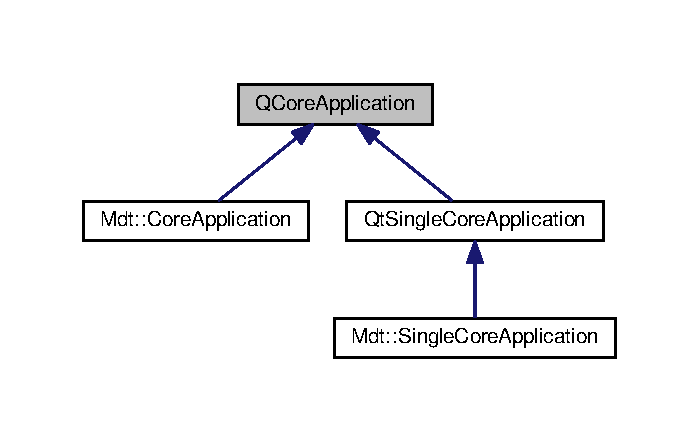
\includegraphics[width=336pt]{class_q_core_application__inherit__graph}
\end{center}
\end{figure}


The documentation for this class was generated from the following file\+:\begin{DoxyCompactItemize}
\item 
libs/\+Qt\+Solutions/\+Qt\+Single\+Application\+\_\+\+Core/src/qtsinglecoreapplication.\+h\end{DoxyCompactItemize}

\hypertarget{class_q_object}{}\section{Q\+Object Class Reference}
\label{class_q_object}\index{Q\+Object@{Q\+Object}}


Inheritance diagram for Q\+Object\+:\nopagebreak
\begin{figure}[H]
\begin{center}
\leavevmode
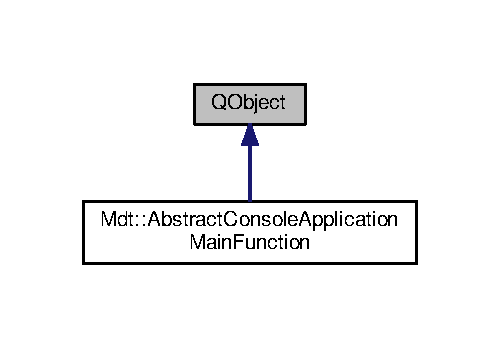
\includegraphics[width=240pt]{class_q_object__inherit__graph}
\end{center}
\end{figure}


The documentation for this class was generated from the following file\+:\begin{DoxyCompactItemize}
\item 
libs/\+Application\+\_\+\+Core/src/\+Mdt/Abstract\+Console\+Application\+Main\+Function.\+h\end{DoxyCompactItemize}

\hypertarget{class_q_shared_data}{}\section{Q\+Shared\+Data Class Reference}
\label{class_q_shared_data}\index{Q\+Shared\+Data@{Q\+Shared\+Data}}


Inheritance diagram for Q\+Shared\+Data\+:
\nopagebreak
\begin{figure}[H]
\begin{center}
\leavevmode
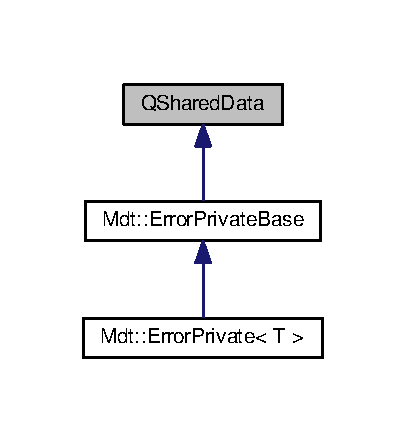
\includegraphics[width=195pt]{class_q_shared_data__inherit__graph}
\end{center}
\end{figure}


The documentation for this class was generated from the following file\+:\begin{DoxyCompactItemize}
\item 
libs/\+Error\+\_\+\+Core/src/\+Mdt/Error.\+h\end{DoxyCompactItemize}

\hypertarget{class_mdt_1_1_standard_paths}{}\section{Mdt\+:\+:Standard\+Paths Class Reference}
\label{class_mdt_1_1_standard_paths}\index{Mdt\+::\+Standard\+Paths@{Mdt\+::\+Standard\+Paths}}


Provides methods for accessing standard paths.  




{\ttfamily \#include $<$Standard\+Paths.\+h$>$}

\subsection*{Static Public Member Functions}
\begin{DoxyCompactItemize}
\item 
static Q\+String \hyperlink{class_mdt_1_1_standard_paths_aa45caeb4d2b4a5c539d301d800a7deac}{log\+Directory\+Path} ()
\begin{DoxyCompactList}\small\item\em Get path to the log file directory. \end{DoxyCompactList}\item 
static Q\+String \hyperlink{class_mdt_1_1_standard_paths_a2ca803e5a6b9fb2a4808968becfb86de}{cache\+Directory\+Path} ()
\begin{DoxyCompactList}\small\item\em Get path to the cache directory. \end{DoxyCompactList}\end{DoxyCompactItemize}


\subsection{Detailed Description}
Provides methods for accessing standard paths. 

This class uses Q\+Standard\+Paths and adds some additionnal paths defined for the \hyperlink{namespace_mdt}{Mdt} library. 

Definition at line 33 of file Standard\+Paths.\+h.



\subsection{Member Function Documentation}
\index{Mdt\+::\+Standard\+Paths@{Mdt\+::\+Standard\+Paths}!cache\+Directory\+Path@{cache\+Directory\+Path}}
\index{cache\+Directory\+Path@{cache\+Directory\+Path}!Mdt\+::\+Standard\+Paths@{Mdt\+::\+Standard\+Paths}}
\subsubsection[{\texorpdfstring{cache\+Directory\+Path()}{cacheDirectoryPath()}}]{\setlength{\rightskip}{0pt plus 5cm}Q\+String Mdt\+::\+Standard\+Paths\+::cache\+Directory\+Path (
\begin{DoxyParamCaption}
{}
\end{DoxyParamCaption}
)\hspace{0.3cm}{\ttfamily [static]}}\hypertarget{class_mdt_1_1_standard_paths_a2ca803e5a6b9fb2a4808968becfb86de}{}\label{class_mdt_1_1_standard_paths_a2ca803e5a6b9fb2a4808968becfb86de}


Get path to the cache directory. 

Returns a path to a writable location located in Q\+Standard\+Paths\+::\+Cache\+Location 

Definition at line 37 of file Standard\+Paths.\+cpp.



Referenced by Mdt\+::\+Core\+Application\+Impl\+::cache\+Directory\+Path().

\index{Mdt\+::\+Standard\+Paths@{Mdt\+::\+Standard\+Paths}!log\+Directory\+Path@{log\+Directory\+Path}}
\index{log\+Directory\+Path@{log\+Directory\+Path}!Mdt\+::\+Standard\+Paths@{Mdt\+::\+Standard\+Paths}}
\subsubsection[{\texorpdfstring{log\+Directory\+Path()}{logDirectoryPath()}}]{\setlength{\rightskip}{0pt plus 5cm}Q\+String Mdt\+::\+Standard\+Paths\+::log\+Directory\+Path (
\begin{DoxyParamCaption}
{}
\end{DoxyParamCaption}
)\hspace{0.3cm}{\ttfamily [static]}}\hypertarget{class_mdt_1_1_standard_paths_aa45caeb4d2b4a5c539d301d800a7deac}{}\label{class_mdt_1_1_standard_paths_aa45caeb4d2b4a5c539d301d800a7deac}


Get path to the log file directory. 

Returns a path to a writable location located in Q\+Standard\+Paths\+::\+App\+Data\+Location/log 

Definition at line 32 of file Standard\+Paths.\+cpp.



Referenced by Mdt\+::\+Core\+Application\+Impl\+::log\+Directory\+Path().



The documentation for this class was generated from the following files\+:\begin{DoxyCompactItemize}
\item 
libs/\+Application\+\_\+\+Core/src/\+Mdt/Standard\+Paths.\+h\item 
libs/\+Application\+\_\+\+Core/src/\+Mdt/Standard\+Paths.\+cpp\end{DoxyCompactItemize}

%--- End generated contents ---

% Index
\backmatter
\newpage
\phantomsection
\clearemptydoublepage
\addcontentsline{toc}{chapter}{Index}
\printindex

\end{document}
